% Generated by Sphinx.
\def\sphinxdocclass{report}
\documentclass[letterpaper,10pt,dvipdfmx]{sphinxmanual}
\usepackage[utf8]{inputenc}
\DeclareUnicodeCharacter{00A0}{\nobreakspace}
\usepackage{cmap}
\usepackage[T1]{fontenc}

\usepackage{times}

\usepackage{longtable}
\usepackage{sphinx}
\usepackage{multirow}


\renewcommand{\figurename}{図 }
\renewcommand{\tablename}{TABLE }
\floatname{literal-block}{LIST }



\title{vhdl2016 Documentation}
\date{}
\release{2016.01.10}
\author{Masayuki Takagiwa}
\newcommand{\sphinxlogo}{}
\renewcommand{\releasename}{リリース}
\makeindex

\makeatletter
\def\PYG@reset{\let\PYG@it=\relax \let\PYG@bf=\relax%
    \let\PYG@ul=\relax \let\PYG@tc=\relax%
    \let\PYG@bc=\relax \let\PYG@ff=\relax}
\def\PYG@tok#1{\csname PYG@tok@#1\endcsname}
\def\PYG@toks#1+{\ifx\relax#1\empty\else%
    \PYG@tok{#1}\expandafter\PYG@toks\fi}
\def\PYG@do#1{\PYG@bc{\PYG@tc{\PYG@ul{%
    \PYG@it{\PYG@bf{\PYG@ff{#1}}}}}}}
\def\PYG#1#2{\PYG@reset\PYG@toks#1+\relax+\PYG@do{#2}}

\expandafter\def\csname PYG@tok@ne\endcsname{\def\PYG@tc##1{\textcolor[rgb]{0.00,0.44,0.13}{##1}}}
\expandafter\def\csname PYG@tok@nf\endcsname{\def\PYG@tc##1{\textcolor[rgb]{0.02,0.16,0.49}{##1}}}
\expandafter\def\csname PYG@tok@si\endcsname{\let\PYG@it=\textit\def\PYG@tc##1{\textcolor[rgb]{0.44,0.63,0.82}{##1}}}
\expandafter\def\csname PYG@tok@m\endcsname{\def\PYG@tc##1{\textcolor[rgb]{0.13,0.50,0.31}{##1}}}
\expandafter\def\csname PYG@tok@nt\endcsname{\let\PYG@bf=\textbf\def\PYG@tc##1{\textcolor[rgb]{0.02,0.16,0.45}{##1}}}
\expandafter\def\csname PYG@tok@ow\endcsname{\let\PYG@bf=\textbf\def\PYG@tc##1{\textcolor[rgb]{0.00,0.44,0.13}{##1}}}
\expandafter\def\csname PYG@tok@sd\endcsname{\let\PYG@it=\textit\def\PYG@tc##1{\textcolor[rgb]{0.25,0.44,0.63}{##1}}}
\expandafter\def\csname PYG@tok@mi\endcsname{\def\PYG@tc##1{\textcolor[rgb]{0.13,0.50,0.31}{##1}}}
\expandafter\def\csname PYG@tok@sx\endcsname{\def\PYG@tc##1{\textcolor[rgb]{0.78,0.36,0.04}{##1}}}
\expandafter\def\csname PYG@tok@go\endcsname{\def\PYG@tc##1{\textcolor[rgb]{0.20,0.20,0.20}{##1}}}
\expandafter\def\csname PYG@tok@ni\endcsname{\let\PYG@bf=\textbf\def\PYG@tc##1{\textcolor[rgb]{0.84,0.33,0.22}{##1}}}
\expandafter\def\csname PYG@tok@c1\endcsname{\let\PYG@it=\textit\def\PYG@tc##1{\textcolor[rgb]{0.25,0.50,0.56}{##1}}}
\expandafter\def\csname PYG@tok@sc\endcsname{\def\PYG@tc##1{\textcolor[rgb]{0.25,0.44,0.63}{##1}}}
\expandafter\def\csname PYG@tok@kn\endcsname{\let\PYG@bf=\textbf\def\PYG@tc##1{\textcolor[rgb]{0.00,0.44,0.13}{##1}}}
\expandafter\def\csname PYG@tok@na\endcsname{\def\PYG@tc##1{\textcolor[rgb]{0.25,0.44,0.63}{##1}}}
\expandafter\def\csname PYG@tok@mh\endcsname{\def\PYG@tc##1{\textcolor[rgb]{0.13,0.50,0.31}{##1}}}
\expandafter\def\csname PYG@tok@gi\endcsname{\def\PYG@tc##1{\textcolor[rgb]{0.00,0.63,0.00}{##1}}}
\expandafter\def\csname PYG@tok@no\endcsname{\def\PYG@tc##1{\textcolor[rgb]{0.38,0.68,0.84}{##1}}}
\expandafter\def\csname PYG@tok@gp\endcsname{\let\PYG@bf=\textbf\def\PYG@tc##1{\textcolor[rgb]{0.78,0.36,0.04}{##1}}}
\expandafter\def\csname PYG@tok@o\endcsname{\def\PYG@tc##1{\textcolor[rgb]{0.40,0.40,0.40}{##1}}}
\expandafter\def\csname PYG@tok@bp\endcsname{\def\PYG@tc##1{\textcolor[rgb]{0.00,0.44,0.13}{##1}}}
\expandafter\def\csname PYG@tok@kd\endcsname{\let\PYG@bf=\textbf\def\PYG@tc##1{\textcolor[rgb]{0.00,0.44,0.13}{##1}}}
\expandafter\def\csname PYG@tok@nn\endcsname{\let\PYG@bf=\textbf\def\PYG@tc##1{\textcolor[rgb]{0.05,0.52,0.71}{##1}}}
\expandafter\def\csname PYG@tok@c\endcsname{\let\PYG@it=\textit\def\PYG@tc##1{\textcolor[rgb]{0.25,0.50,0.56}{##1}}}
\expandafter\def\csname PYG@tok@gu\endcsname{\let\PYG@bf=\textbf\def\PYG@tc##1{\textcolor[rgb]{0.50,0.00,0.50}{##1}}}
\expandafter\def\csname PYG@tok@k\endcsname{\let\PYG@bf=\textbf\def\PYG@tc##1{\textcolor[rgb]{0.00,0.44,0.13}{##1}}}
\expandafter\def\csname PYG@tok@nl\endcsname{\let\PYG@bf=\textbf\def\PYG@tc##1{\textcolor[rgb]{0.00,0.13,0.44}{##1}}}
\expandafter\def\csname PYG@tok@w\endcsname{\def\PYG@tc##1{\textcolor[rgb]{0.73,0.73,0.73}{##1}}}
\expandafter\def\csname PYG@tok@se\endcsname{\let\PYG@bf=\textbf\def\PYG@tc##1{\textcolor[rgb]{0.25,0.44,0.63}{##1}}}
\expandafter\def\csname PYG@tok@ge\endcsname{\let\PYG@it=\textit}
\expandafter\def\csname PYG@tok@ss\endcsname{\def\PYG@tc##1{\textcolor[rgb]{0.32,0.47,0.09}{##1}}}
\expandafter\def\csname PYG@tok@vg\endcsname{\def\PYG@tc##1{\textcolor[rgb]{0.73,0.38,0.84}{##1}}}
\expandafter\def\csname PYG@tok@mo\endcsname{\def\PYG@tc##1{\textcolor[rgb]{0.13,0.50,0.31}{##1}}}
\expandafter\def\csname PYG@tok@nd\endcsname{\let\PYG@bf=\textbf\def\PYG@tc##1{\textcolor[rgb]{0.33,0.33,0.33}{##1}}}
\expandafter\def\csname PYG@tok@cs\endcsname{\def\PYG@tc##1{\textcolor[rgb]{0.25,0.50,0.56}{##1}}\def\PYG@bc##1{\setlength{\fboxsep}{0pt}\colorbox[rgb]{1.00,0.94,0.94}{\strut ##1}}}
\expandafter\def\csname PYG@tok@kc\endcsname{\let\PYG@bf=\textbf\def\PYG@tc##1{\textcolor[rgb]{0.00,0.44,0.13}{##1}}}
\expandafter\def\csname PYG@tok@mf\endcsname{\def\PYG@tc##1{\textcolor[rgb]{0.13,0.50,0.31}{##1}}}
\expandafter\def\csname PYG@tok@sh\endcsname{\def\PYG@tc##1{\textcolor[rgb]{0.25,0.44,0.63}{##1}}}
\expandafter\def\csname PYG@tok@nc\endcsname{\let\PYG@bf=\textbf\def\PYG@tc##1{\textcolor[rgb]{0.05,0.52,0.71}{##1}}}
\expandafter\def\csname PYG@tok@sr\endcsname{\def\PYG@tc##1{\textcolor[rgb]{0.14,0.33,0.53}{##1}}}
\expandafter\def\csname PYG@tok@gr\endcsname{\def\PYG@tc##1{\textcolor[rgb]{1.00,0.00,0.00}{##1}}}
\expandafter\def\csname PYG@tok@kt\endcsname{\def\PYG@tc##1{\textcolor[rgb]{0.56,0.13,0.00}{##1}}}
\expandafter\def\csname PYG@tok@gt\endcsname{\def\PYG@tc##1{\textcolor[rgb]{0.00,0.27,0.87}{##1}}}
\expandafter\def\csname PYG@tok@s1\endcsname{\def\PYG@tc##1{\textcolor[rgb]{0.25,0.44,0.63}{##1}}}
\expandafter\def\csname PYG@tok@vc\endcsname{\def\PYG@tc##1{\textcolor[rgb]{0.73,0.38,0.84}{##1}}}
\expandafter\def\csname PYG@tok@gd\endcsname{\def\PYG@tc##1{\textcolor[rgb]{0.63,0.00,0.00}{##1}}}
\expandafter\def\csname PYG@tok@mb\endcsname{\def\PYG@tc##1{\textcolor[rgb]{0.13,0.50,0.31}{##1}}}
\expandafter\def\csname PYG@tok@s\endcsname{\def\PYG@tc##1{\textcolor[rgb]{0.25,0.44,0.63}{##1}}}
\expandafter\def\csname PYG@tok@vi\endcsname{\def\PYG@tc##1{\textcolor[rgb]{0.73,0.38,0.84}{##1}}}
\expandafter\def\csname PYG@tok@il\endcsname{\def\PYG@tc##1{\textcolor[rgb]{0.13,0.50,0.31}{##1}}}
\expandafter\def\csname PYG@tok@kp\endcsname{\def\PYG@tc##1{\textcolor[rgb]{0.00,0.44,0.13}{##1}}}
\expandafter\def\csname PYG@tok@err\endcsname{\def\PYG@bc##1{\setlength{\fboxsep}{0pt}\fcolorbox[rgb]{1.00,0.00,0.00}{1,1,1}{\strut ##1}}}
\expandafter\def\csname PYG@tok@nv\endcsname{\def\PYG@tc##1{\textcolor[rgb]{0.73,0.38,0.84}{##1}}}
\expandafter\def\csname PYG@tok@s2\endcsname{\def\PYG@tc##1{\textcolor[rgb]{0.25,0.44,0.63}{##1}}}
\expandafter\def\csname PYG@tok@cm\endcsname{\let\PYG@it=\textit\def\PYG@tc##1{\textcolor[rgb]{0.25,0.50,0.56}{##1}}}
\expandafter\def\csname PYG@tok@gh\endcsname{\let\PYG@bf=\textbf\def\PYG@tc##1{\textcolor[rgb]{0.00,0.00,0.50}{##1}}}
\expandafter\def\csname PYG@tok@sb\endcsname{\def\PYG@tc##1{\textcolor[rgb]{0.25,0.44,0.63}{##1}}}
\expandafter\def\csname PYG@tok@nb\endcsname{\def\PYG@tc##1{\textcolor[rgb]{0.00,0.44,0.13}{##1}}}
\expandafter\def\csname PYG@tok@kr\endcsname{\let\PYG@bf=\textbf\def\PYG@tc##1{\textcolor[rgb]{0.00,0.44,0.13}{##1}}}
\expandafter\def\csname PYG@tok@gs\endcsname{\let\PYG@bf=\textbf}
\expandafter\def\csname PYG@tok@cp\endcsname{\def\PYG@tc##1{\textcolor[rgb]{0.00,0.44,0.13}{##1}}}

\def\PYGZbs{\char`\\}
\def\PYGZus{\char`\_}
\def\PYGZob{\char`\{}
\def\PYGZcb{\char`\}}
\def\PYGZca{\char`\^}
\def\PYGZam{\char`\&}
\def\PYGZlt{\char`\<}
\def\PYGZgt{\char`\>}
\def\PYGZsh{\char`\#}
\def\PYGZpc{\char`\%}
\def\PYGZdl{\char`\$}
\def\PYGZhy{\char`\-}
\def\PYGZsq{\char`\'}
\def\PYGZdq{\char`\"}
\def\PYGZti{\char`\~}
% for compatibility with earlier versions
\def\PYGZat{@}
\def\PYGZlb{[}
\def\PYGZrb{]}
\makeatother

\renewcommand\PYGZsq{\textquotesingle}

\begin{document}

\maketitle
\tableofcontents
\phantomsection\label{index::doc}


Contents:


\chapter{はじめに}
\label{01_introduction:id1}\label{01_introduction::doc}
本書の目的はVHDL によるFPGA (CPLD) への論理回路の実装を一通り体験することです。

到達目標に、「VHDL によるストップウォッチの実装」を設定し、VHDL の説明と実習を行います。

八戸高専の場合、「ディジタル回路」「ディジタル回路」「ディジタル信号処理」と重複するところがあります。それらの授業で学んだことが実習の助けになるでしょう。


\section{受講にあたって}
\label{01_introduction:id2}
以下の点に注意、協力してください。
\begin{itemize}
\item {} 
お昼休みには基板の電源を切ってください。変な回路を書き込んでおいてデバイスに負荷をかけて壊してしまうことを避けるためです。

\item {} 
演習 = このテキスト通りに入力して動作を確認するもの、課題 = 自力でコードを書いて動作させるもの、としています。

\item {} 
演習、課題でどうしてもツールのエラーが消せないときは呼んでください。

\item {} 
課題はできあがったら基板を持って見せに来てください。達成度を記録します。

\item {} 
成績は、課題の達成度と筆記試験から求めます。

\item {} 
筆記試験は最終日に行い、テキストなどの持ち込みは不可です。

\item {} 
欠席せざるを得ないことがあると思います。そのとき課題は授業中、どうにもならないときは後からおこなってください。

\end{itemize}


\chapter{ストップウォッチについて}
\label{02_stopwatch:id1}\label{02_stopwatch::doc}
デジタルタイプのストップウォッチの例を図に示します。通常「スタート・ストップ」「ラップ・リセット」の2つのボタンと、6桁程度の数字のディスプレイがあります。

「スタート・ストップ」のボタンは、押す毎に「計時」の実行、停止が切り替わります。リセットしない限り、計時は停止した値から再開されます。

「ラップ・リセット」は、停止時に押すと値がクリアされます。計時を行っているときに押すと、通常計時中は変化し続けている数字が停止しますが、計時は続けられています。

実際にはここでは2つの動作があり、「スプリット」では値は引き続きカウントアップしていますが、「ラップ」ではラップボタンで計時は0から再開されます。

数字のディスプレイは通常上位から2桁ずつ、分、秒、1/100 秒のカウントを表示します。


\section{実装目標}
\label{02_stopwatch:id2}
最低限の目標は以下の機能をVHDL で実装することです。
\begin{description}
\item[{4桁の数字の表示}] \leavevmode
上位2桁は秒、下位2桁は1/100 秒です。

\item[{「スタート・ストップ」スイッチの動作}] \leavevmode
一つのスイッチで行います。

\item[{「ラップ・リセット」スイッチはリセット動作の実装}] \leavevmode
停止中に値のリセットが行えること。

\end{description}

追加目標はラップ機能、スプリット機能の実装となります。


\chapter{FPGA について}
\label{03_fpga::doc}\label{03_fpga:fpga}
デジタル回路の最小単位は、AND、OR、NOT 等の論理素子で、さらにこれらを組み合わせたXOR とフリップフロップが多用されます。これらの単機能デバイス(たとえば16 ピンのIC など)は多く販売されていました。

プロセッサやメモリなどは大規模なデジタル回路で、上記のような機能を組み合わせてIC 、LSI という形で設計されます。

1990 年代中盤のプロセッサやメモリは単体では機能が少なく、基板上で、上記のような単機能デバイスを組み合わせたサポート回路が必要となっていました。

これらのサポート回路をまた新しいIC 、LSI で設計することも可能でしたが、対象となるCPU や、基板が対象としている機能などで必要となる回路が異なるため、現実的ではありませんでした。

ちなみに小規模なIC 、LSI でも実際のデバイスにするまでに数千万から億単位の費用がかかるそうです。

そこで、大量の論理素子と、それらをつなぐ大量の配線+スイッチをあらかじめIC 内に作り込んでおき、素子、スイッチ毎にON、OFF を設定することで、まるで専用のICのように使おうという考えが生まれ、そのようなデバイスが作られました。

これがFPGA の始まりとなります。

IC 、LSI の技術の進歩とともに規模も大きくなり、動作速度も高くなり、現在ではただのサポート回路にとどまらず、信号処理の分野でも使われています。

性能や価格では、億単位の費用をかけたLSI にはかなわないため、そういった対応ができない分野で多く使われています。

例:
\begin{description}
\item[{製品の初期開発}] \leavevmode
たとえば第3世代携帯電話の端末、基地局の開発は、世界標準の規格がまだ確定していない時期から始まっているため、後から変更が必要な可能性がとても高い状態でした。そのため、あとから内容を変更できるよう基板はFPGA を搭載して製造しておき、仕様変更があってもすぐ対応できるようにします(LSI では製造にも時間がかかります)。

\item[{特殊な信号処理装置}] \leavevmode
たとえば金融取引向けには一般のパソコンにも組み込める、単にFPGA が載っているだけの基板が使われます。内容は会社それぞれが独自のノウハウで設計するため、全てのユーザ共通とはできないので、空っぽのままで販売されます。

\end{description}

\begin{notice}{note}{注釈:}
実際にこの授業で使用するデバイスは「PLD」と呼ばれます。PLD は Programmable Logic Device の略です。プログラム可能な論理デバイス、となります。

対してFPGA はField Programmable Gate Array の略です。現場(Field)でプログラム可能なゲート(論理)の集合、となります。

できることはほぼ同じですが、以下のような特徴で分けています。

CPLD
\begin{itemize}
\item {} 
フラッシュメモリを内蔵し、電源を入れるとすぐ使える。

\item {} 
回路規模は小さめ。

\item {} 
基本的に論理回路しか入ってない。

\item {} 
動作速度が比較的高い。

\item {} 
構造上、XOR が少し苦手。

\end{itemize}

FPGA
\begin{itemize}
\item {} 
動作のプログラムは揮発性のメモリに格納されるので、電源を切ると内容が失われる。そのため別途フラッシュメモリが必要。

\item {} 
回路規模はかなり大きい。

\item {} 
高機能(乗算用ハードウェアが入っていたり、メモリが入っていたりする)。

\item {} 
動作速度は今ではだいぶ高くなってきた。

\end{itemize}

それぞれのデバイスの構成要素は以下の図のようになっています。いずれもD フリップフロップと組み合わせ回路がセットになっており、その入力をプログラムするような形です。このセットがデバイスの中に多数組み込まれ、相互に接続できるよう配線とスイッチも同様に多数用意されます。

CPLD とFPGA の間の大きな違いは組み合わせ回路の構成です。CPLD は大量の ANDと多入力 OR を組み合わせていますが(実際には NOT も入ります)、FPGA は AND 、OR に縛られない LUT (LookUp Table) を使用します。たとえば4入力の AND 、4入力の OR に限らず、''4'' 等の任意の数値と一致したときに H を出力する、というようなことも簡単にできるよう、より柔軟な構造になっています。

いずれの場合でもD フリップフロップが既に組み込まれていますので、AND を組み合わせたようなフリップフロップを改めて記述する必要はなく、むしろ期待通りに動作しない可能性があります。
\end{notice}


\section{3.1 HDL}
\label{03_fpga:hdl}
ディジタル回路を組み込んだIC やLSI の開発では、初期にはAND 、OR 、NOT 、フリップフロップをCAD 上で回路図のように配置して接続していました。

こういったCAD は、IC 、LSI メーカー毎に異なるため、たとえば完成したデータを違うLSI メーカーで製造しなければいけなくなったとき、互換性が無いため入力&確認し直しが必要になっていました。

こういった状況を避けるために、IC 、LSI の開発も、ソフトウェアのようにテキストで行おうという動きがでてきました。このジャンルの言語はHDL (Hardware Description Language)と呼ばれます。

ソフトウェアと同様、HDL も様々なものが開発されましたが、現在の主流はVerilogHDLとVHDL です。

\begin{notice}{note}{注釈:}
HDL は一般にソフトウェアとは異なる考え方が必要になります。それだけ、ソフトウェアのプログラマに比べ人口が少ないです。
現在ソフトウェアの開発環境は無料で入手できるようになり、早ければ小学生から始める人もいます。
特に研究の分野ではFPGA に興味を持つ方は多いのですが、開発環境やサンプルボードが高価なこともあり、独学で覚えられる環境は多くありませんでした。
HDL を多少でも理解できると、その分対応できる仕事が広がります。ただ、通常のC 言語をベースにもっとたくさんの人がFPGA 開発できるようにする動きも以前からあり、少しずつ成果が出始めてきています。
\end{notice}


\section{3.2 VerilogHDL とVHDL}
\label{03_fpga:veriloghdl-vhdl}
各言語の特徴を以下に示します(筆者の独断と偏見を含む)

VerilogHDL
\begin{itemize}
\item {} 
民間主導- ツールメーカーが開発した。

\item {} 
比較的便利な記述ができるようになっている。

\item {} 
文法上記述ミスが許容される傾向がある= デバッグ時に大変なことが多い。

\item {} 
日本でのシェアは、こちらがかすかに多いかもしれない。

\item {} 
C 言語に近い、と評されることがあるものの、上記のような動きがあることから、むしろBASIC の方が近いと感じる。

\item {} 
無料のシミュレータがあるため、特に趣味の範囲での人気はVHDL より高い模様。

\end{itemize}

VHDL
\begin{itemize}
\item {} 
米国国防省主導- ソフトウェアのプログラミング言語をベースに策定

\item {} 
融通が利かず、あまり高機能でない。コード量は多くなる傾向かもしれない。

\item {} 
海外でのシェアは、こちらがかすかに多いかもしれない。

\item {} 
BASIC ににたキーワードもあるものの、文法エラーの検出の強さはC 言語に近い。

\end{itemize}


\chapter{VHDL}
\label{04_vhdl::doc}\label{04_vhdl:vhdl}

\section{4.1 基本形}
\label{04_vhdl:id1}
VHDL のソースコードは、基本的には以下のような形です。
\begin{figure}[htbp]
\centering

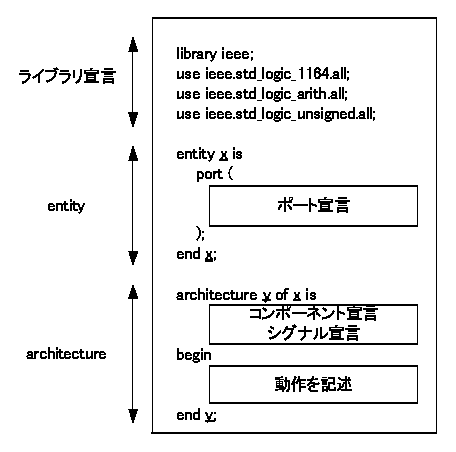
\includegraphics{figure01.eps}
\end{figure}

これがテンプレートとなります。コードを記述するときは、この中の x、y、3つの枠の中を、目的に合わせて書き換えます。

ここで x は entity 名、y は architecture 名です。ポート宣言はこの entity が外部とやりとりする信号(たとえば実際のデバイスのピン)を宣言します。

entity 名はこの回路に対する自由な名前(たとえば機能から名付けるなど)、architecture名はどの entity に対しても同じ「rtl」という名前をつけておけば通常問題ありません。

これらは以下のようなイメージになります。
\begin{figure}[htbp]
\centering

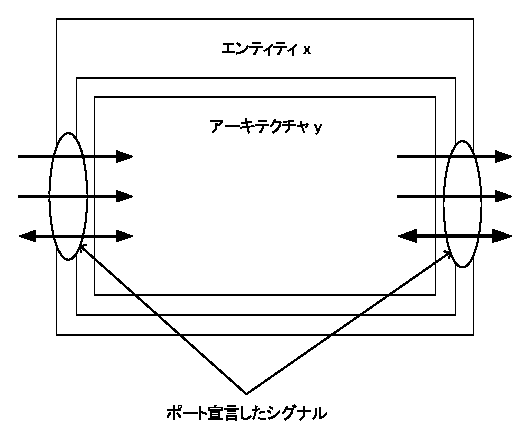
\includegraphics{figure02.eps}
\end{figure}

ファイルにはいくつかの entity 、architecture を含めることができますが、この実習では一つのファイルに一つの entity 、architecture を保存し、ファイル名は entity 名に合わせて設定してください。
\begin{figure}[htbp]
\centering

\includegraphics{figure03.eps}
\end{figure}


\subsection{4.1.1 解説}
\label{04_vhdl:id2}

\subsubsection{4.1.1.1 entity とその周辺}
\label{04_vhdl:entity}
entity と architecture はいずれもそれ単体では何もできません。わざわざ分かれているところから想像できるとおり、同じ entity に対して異なる architecture を適用させることもできますが、この授業では扱いません。

また entity 、architecture が動作するためには、entity の前にある4行のライブラリ宣言が必要です。

ここでは ieee の 1164 、arith 、unsigned を呼び出しています。この授業ではこの組み合わせを使用しますので、この4行のライブラリ宣言もそのまま使用します。

C 言語のインクルードファイルの宣言などと異なり、ファイルに複数の entity 、architecture を記述する場合、ライブラリ宣言は entity 毎に宣言し直す必要があります。4個の entity を記述していれば、その都度、合計4回のライブラリ宣言が必要です。


\subsection{4.1.2 ファイルとの関係}
\label{04_vhdl:id3}
一般にファイル名と entity 名をそろえ、拡張子は「.vhd」とします。

一つのファイルに複数の entity 、architecture を記述することもできますが、その際はそれに対応した use 、library の宣言も必要です。

この授業では、一つのファイルに一つの entity 、architecture とするのがよいでしょう。

またライブラリのうち unsigned は名前から想像できるとおり符号なしの演算を行います。符号付きの演算を行いたい場合は代わりに signed を呼び出します。一つの entity 、architecture 内では混在はできません。


\section{4.2 信号の種類}
\label{04_vhdl:id4}
信号は、ソフトウェアで言う変数と同様のイメージから考えてください。

たとえば C 言語であれば char 、int 、float 等があるように、VHDL でもライブラリを読み込むことで以下のような信号が扱えます。


\subsection{4.2.1 std\_logic}
\label{04_vhdl:std-logic}
1bit の信号。通常使用する値は 0、1、Z です。

直値を扱う場合、1bit 分ずつシングルクオートで括ります。

0、1 は信号の L レベル、 H レベルに対応します。

Z は「ハイインピーダンス」で、その信号が無い、何もつながっていない状態を作ります。この授業の範囲では使いません。

例

\begin{Verbatim}[commandchars=\\\{\}]
\PYG{p}{\PYGZsq{}} \PYG{l+m+mi}{0} \PYG{p}{\PYGZsq{}} \PYG{p}{,} \PYG{p}{\PYGZsq{}} \PYG{l+m+mi}{1} \PYG{p}{\PYGZsq{}} \PYG{p}{,} \PYG{n+na}{\PYGZsq{}Z} \PYG{p}{\PYGZsq{}}
\end{Verbatim}


\subsection{4.2.2 std\_logic\_vector}
\label{04_vhdl:std-logic-vector}
std\_logic を束ねたもので、任意のビット数を扱うことができます。

各ビットに代入できる値は std\_logic と同じです。

束ねるビット数は宣言時に決めておきます。たとえば10進数で0~100までを扱うには 7bit 必要ですので、7本の std\_logic を束ねるため、以下のような形式になります。

\begin{Verbatim}[commandchars=\\\{\}]
\PYG{k+kt}{std\PYGZus{}logic\PYGZus{}vector}\PYG{p}{(}\PYG{l+m+mi}{6} \PYG{k}{downto} \PYG{l+m+mi}{0}\PYG{p}{)}
\end{Verbatim}

この場合、MSB \footnote[1]{
変化することにより全体の値が大きく変化するビット
} が bit 6 、LSB \footnote[2]{
変化から値全体の変化が一番小さいビット
} が bit 0 という宣言になります。ここに代入する値は、たとえば10進数の10であれば

\begin{Verbatim}[commandchars=\\\{\}]
\PYG{l+s}{\PYGZdq{}0001010\PYGZdq{}}
\end{Verbatim}

というふうにダブルクオーテーションで括ります。左が bit6 、右が bit0 です。代入する値は、代入先の信号とビット幅が一致している必要があります \footnote[3]{
ビット幅が一致していなくてもツール上エラーにならない場合があり、発見しづらいバグになりやすいです。
} 。

例

\begin{Verbatim}[commandchars=\\\{\}]
\PYG{l+s}{\PYGZdq{}0000\PYGZdq{}, \PYGZdq{}010101010\PYGZdq{}, \PYGZdq{}00Z00Z\PYGZdq{}}
\end{Verbatim}

括弧()でビット番号を指定することで、std\_logic として 1bit 抜き出して扱うことができます。

\begin{notice}{note}{注釈:}
std\_logic\_vector(0 to 6) という宣言の仕方もありますが、ソースやプロジェクトの中で混在させるのはバグのもとになるので通常はどちらかに統一します。

この授業では downto に統一します。

図の上を MSB、下を LSB とした場合、downto と to の関係は次の図のようになります。
\begin{figure}[htbp]
\centering

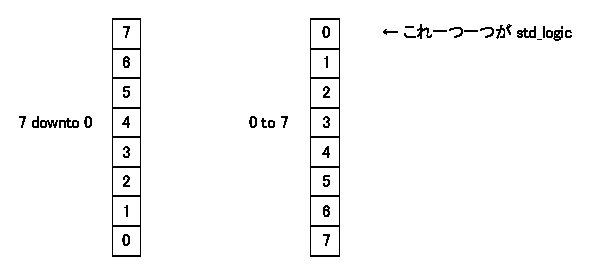
\includegraphics{figure04.eps}
\end{figure}
\end{notice}


\subsection{4.2.3 integer}
\label{04_vhdl:integer}
10 進数を直接扱います。bit は意識しません。std\_logic や std\_logic\_vector とは直接接続することはできません。


\section{4.3 ポート宣言}
\label{04_vhdl:id8}
ポート宣言では、この entity (回路ブロック)が外部とやりとりする信号を定義します。

複数の信号を定義でき、それぞれ以下のような形です。

ポート名: 方向信号型

定義の区切りにセミコロンが必要です。定義の終わりを示すものでは無いので、最後の定義ではセミコロンは書きません。

例

\begin{Verbatim}[commandchars=\\\{\}]
\PYG{n}{extsignal1} \PYG{o}{:} \PYG{k}{in} \PYG{k+kt}{std\PYGZus{}logic}\PYG{p}{;}
\PYG{n}{extsignal2} \PYG{o}{:} \PYG{k}{out} \PYG{k+kt}{std\PYGZus{}logic\PYGZus{}vector}\PYG{p}{(}\PYG{l+m+mi}{3} \PYG{k}{downto} \PYG{l+m+mi}{0}\PYG{p}{)}\PYG{p}{;}
\PYG{n}{extsignal3} \PYG{o}{:} \PYG{k}{inout} \PYG{k+kt}{std\PYGZus{}logic}\PYG{p}{;}
\PYG{n}{extsignal4} \PYG{o}{:} \PYG{k}{buffer} \PYG{k+kt}{std\PYGZus{}logic}
\end{Verbatim}

ポート名は任意の名前をつけ、architecture 内からその信号にアクセスできます。

方向については上記の4パターンがあります。
\begin{description}
\item[{in}] \leavevmode
この entity への入力です。architecture 内では読むことしかできません。

\item[{out}] \leavevmode
この entity からの出力です。architecture 内で書き込むことしかできません。

\item[{inout}] \leavevmode
入出力両方ができます。architecture 内では読み書きができますが、信号が衝突すると電気的に短絡(ショート)となるため、エラーとなります。エラーにならない対応はこの授業では扱いません。

\item[{buffer}] \leavevmode
この entity からの出力です。out との違いは信号の再利用ができることですが、制約もあるので使うのは避けた方がよいでしょう。

\end{description}

それぞれのイメージを図に示します。読み書きは他の signal へ、または signal からの「代入」と読み替えてもよいでしょう。

buffer と inout はこの授業では使用しません。
\begin{figure}[htbp]
\centering

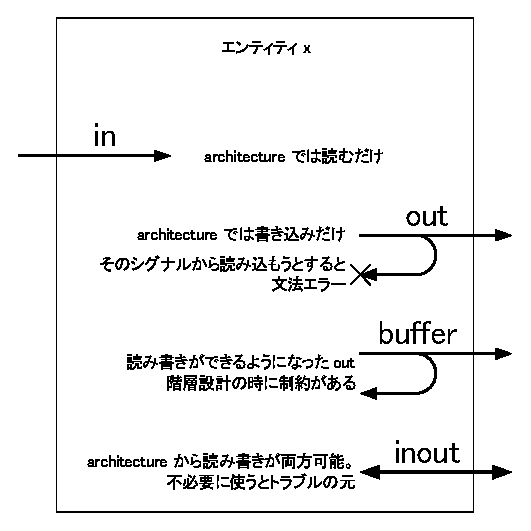
\includegraphics{figure05.eps}
\end{figure}


\section{4.4 シグナル宣言}
\label{04_vhdl:id9}
アーキテクチャの中で使用する信号を宣言します。アーキテクチャの記述の中で、beginの前に行います(begin より後には宣言できません)。

例

\begin{Verbatim}[commandchars=\\\{\}]
\PYG{k}{signal} \PYG{n}{intsignal1} \PYG{o}{:} \PYG{k+kt}{std\PYGZus{}logic}\PYG{p}{;}
\PYG{k}{signal} \PYG{n}{intsignal2} \PYG{o}{:} \PYG{k+kt}{std\PYGZus{}logic\PYGZus{}vector}\PYG{p}{(}\PYG{l+m+mi}{3} \PYG{k}{downto} \PYG{l+m+mi}{0}\PYG{p}{)}\PYG{p}{;}
\PYG{k}{signal} \PYG{n}{intsignal3} \PYG{o}{:} \PYG{k+kt}{integer}\PYG{p}{;}
\PYG{k}{signal} \PYG{n}{intsignal4} \PYG{o}{:} \PYG{k+kt}{std\PYGZus{}logic}\PYG{p}{;}
\end{Verbatim}

``signal'' キーワードの後に、ポート宣言と同様に任意の名前をつけます。信号の種類もポート宣言と同様です。

アーキテクチャ内部でのみ使用するので、方向は記述しません。

また全ての宣言で末尾はセミコロンで閉じます。


\section{4.5 値の代入}
\label{04_vhdl:id10}
代入は ``\textless{}='' で行います。

例(1)

\begin{Verbatim}[commandchars=\\\{\}]
\PYG{n}{intsignal1} \PYG{o}{\PYGZlt{}}\PYG{o}{=} \PYG{l+s+sc}{\PYGZsq{}1\PYGZsq{}}\PYG{p}{;}
\PYG{n}{intsignal4} \PYG{o}{\PYGZlt{}}\PYG{o}{=} \PYG{n}{intesignal1}\PYG{p}{;}
\PYG{n}{intsignal2} \PYG{o}{\PYGZlt{}}\PYG{o}{=} \PYG{l+s}{\PYGZdq{}0000\PYGZdq{}}\PYG{p}{;}
\PYG{n}{intsignal3} \PYG{o}{\PYGZlt{}}\PYG{o}{=} \PYG{l+m+mi}{5}\PYG{p}{;}
\end{Verbatim}

std\_logic\_vector の場合は値の扱い方にバリエーションがあるのでここで解説します。

合計したビット数が代入先の信号に一致していれば、&で結合できます。

括弧でビットを指定すれば、std\_logic を代入したり、参照したりできます。


\section{4.6 もう一つの信号 variable と代入}
\label{04_vhdl:variable}
VHDL には port 、signal の他にもう一つ、variable という信号のタイプがあります。

variable は後述する process 文の中でのみ使用でき、信号のタイプは他と同様 std\_logic 等を使うことができます。

代入には := を使います。

variable はこの授業では扱いません。


\chapter{第5章 演習}
\label{05_try:id1}\label{05_try::doc}

\section{5.1 注意事項}
\label{05_try:id2}\begin{itemize}
\item {} 
開発環境 Quatus II のプロジェクトは、実習項目毎に作り直してください。流用するとトラブルの元になります。

\item {} 
Quatus II の中で日本語を入力するのは避けましょう。こちらもトラブルの元になります。

\end{itemize}


\section{5.2 論理演算}
\label{05_try:id3}

\subsection{5.2.1 演習}
\label{05_try:id4}
プロジェクト名 vhdl01

スイッチ入力に対して論理演算を行い、結果を LED に出力します。

\begin{Verbatim}[commandchars=\\\{\}]
\PYG{k}{library} \PYG{n+nn}{ieee}\PYG{p}{;}
\PYG{k}{use} \PYG{n+nn}{ieee.std\PYGZus{}logic\PYGZus{}1164.all}\PYG{p}{;}
\PYG{k}{use} \PYG{n+nn}{ieee.std\PYGZus{}logic\PYGZus{}arith.all}\PYG{p}{;}
\PYG{k}{use} \PYG{n+nn}{ieee.std\PYGZus{}logic\PYGZus{}unsigned.all}\PYG{p}{;}

\PYG{k}{entity} \PYG{n+nc}{vhdl01} \PYG{k}{is}
  \PYG{k}{port} \PYG{p}{(}
    \PYG{n}{sw1}  \PYG{o}{:} \PYG{k}{in} \PYG{k+kt}{std\PYGZus{}logic}\PYG{p}{;}
    \PYG{n}{sw2}  \PYG{o}{:} \PYG{k}{in} \PYG{k+kt}{std\PYGZus{}logic}\PYG{p}{;}
    \PYG{n}{led1} \PYG{o}{:} \PYG{k}{out} \PYG{k+kt}{std\PYGZus{}logic}\PYG{p}{;}
    \PYG{n}{led2} \PYG{o}{:} \PYG{k}{out} \PYG{k+kt}{std\PYGZus{}logic}\PYG{p}{;}
    \PYG{n}{led3} \PYG{o}{:} \PYG{k}{out} \PYG{k+kt}{std\PYGZus{}logic}\PYG{p}{;}
    \PYG{n}{led4} \PYG{o}{:} \PYG{k}{out} \PYG{k+kt}{std\PYGZus{}logic}\PYG{p}{;}
    \PYG{n}{led5} \PYG{o}{:} \PYG{k}{out} \PYG{k+kt}{std\PYGZus{}logic}
  \PYG{p}{)}\PYG{p}{;}
\PYG{k}{end} \PYG{n+nc}{vhdl01}\PYG{p}{;}

\PYG{k}{architecture} \PYG{n+nc}{rtl} \PYG{k}{of} \PYG{n+nc}{vhdl01} \PYG{k}{is}
\PYG{k}{begin}
  \PYG{n}{led1} \PYG{o}{\PYGZlt{}}\PYG{o}{=} \PYG{n}{sw1}\PYG{p}{;}
  \PYG{n}{led2} \PYG{o}{\PYGZlt{}}\PYG{o}{=} \PYG{n}{sw2}\PYG{p}{;}
  \PYG{n}{led3} \PYG{o}{\PYGZlt{}}\PYG{o}{=} \PYG{n}{sw1} \PYG{k}{and} \PYG{n}{sw2}\PYG{p}{;}
  \PYG{n}{led4} \PYG{o}{\PYGZlt{}}\PYG{o}{=} \PYG{n}{sw1} \PYG{k}{or} \PYG{n}{sw2}\PYG{p}{;}
  \PYG{n}{led5} \PYG{o}{\PYGZlt{}}\PYG{o}{=} \PYG{k}{not} \PYG{n}{sw1}\PYG{p}{;}
\PYG{k}{end} \PYG{n+nc}{rtl}\PYG{p}{;}
\end{Verbatim}

このコードで出力される回路は図のようなものになります。
\begin{figure}[htbp]
\centering

\includegraphics{figure06.eps}
\end{figure}

スイッチは基板奥の方(7セグLED 側)に倒すとH 、手前でL のレベルになります。
LED に対してはデバイスからH を与えると消灯、L を与えると点灯します。
たとえばled1 はスイッチ1番を奥に倒すと消灯、手前に倒すと点灯します。led5 は逆の点灯の仕方になります。


\section{5.3 数値演算}
\label{05_try:id5}

\subsection{5.3.1 演習}
\label{05_try:id6}
プロジェクト名 vhdl02

スイッチ入力に対して数値演算を行い、LED に表示します。

\begin{Verbatim}[commandchars=\\\{\}]
\PYG{k}{library} \PYG{n+nn}{ieee}\PYG{p}{;}
\PYG{k}{use} \PYG{n+nn}{ieee.std\PYGZus{}logic\PYGZus{}1164.all}\PYG{p}{;}
\PYG{k}{use} \PYG{n+nn}{ieee.std\PYGZus{}logic\PYGZus{}arith.all}\PYG{p}{;}
\PYG{k}{use} \PYG{n+nn}{ieee.std\PYGZus{}logic\PYGZus{}unsigned.all}\PYG{p}{;}

\PYG{k}{entity} \PYG{n+nc}{vhdl02} \PYG{k}{is}
  \PYG{k}{port} \PYG{p}{(}
    \PYG{n}{sw1} \PYG{o}{:} \PYG{k}{in} \PYG{k+kt}{std\PYGZus{}logic}\PYG{p}{;}
    \PYG{n}{sw2} \PYG{o}{:} \PYG{k}{in} \PYG{k+kt}{std\PYGZus{}logic}\PYG{p}{;}
    \PYG{n}{sw3} \PYG{o}{:} \PYG{k}{in} \PYG{k+kt}{std\PYGZus{}logic}\PYG{p}{;}
    \PYG{n}{sw4} \PYG{o}{:} \PYG{k}{in} \PYG{k+kt}{std\PYGZus{}logic}\PYG{p}{;}
    \PYG{n}{sw5} \PYG{o}{:} \PYG{k}{in} \PYG{k+kt}{std\PYGZus{}logic}\PYG{p}{;}
    \PYG{n}{sw6} \PYG{o}{:} \PYG{k}{in} \PYG{k+kt}{std\PYGZus{}logic}\PYG{p}{;}
    \PYG{n}{sw7} \PYG{o}{:} \PYG{k}{in} \PYG{k+kt}{std\PYGZus{}logic}\PYG{p}{;}
    \PYG{n}{sw8} \PYG{o}{:} \PYG{k}{in} \PYG{k+kt}{std\PYGZus{}logic}\PYG{p}{;}

    \PYG{n}{led1} \PYG{o}{:} \PYG{k}{out} \PYG{k+kt}{std\PYGZus{}logic}\PYG{p}{;}
    \PYG{n}{led2} \PYG{o}{:} \PYG{k}{out} \PYG{k+kt}{std\PYGZus{}logic}\PYG{p}{;}
    \PYG{n}{led3} \PYG{o}{:} \PYG{k}{out} \PYG{k+kt}{std\PYGZus{}logic}\PYG{p}{;}
    \PYG{n}{led4} \PYG{o}{:} \PYG{k}{out} \PYG{k+kt}{std\PYGZus{}logic}\PYG{p}{;}
    \PYG{n}{led5} \PYG{o}{:} \PYG{k}{out} \PYG{k+kt}{std\PYGZus{}logic}\PYG{p}{;}
    \PYG{n}{led6} \PYG{o}{:} \PYG{k}{out} \PYG{k+kt}{std\PYGZus{}logic}\PYG{p}{;}
    \PYG{n}{led7} \PYG{o}{:} \PYG{k}{out} \PYG{k+kt}{std\PYGZus{}logic}\PYG{p}{;}
    \PYG{n}{led8} \PYG{o}{:} \PYG{k}{out} \PYG{k+kt}{std\PYGZus{}logic}\PYG{p}{;}

    \PYG{n}{sled1a} \PYG{o}{:} \PYG{k}{out} \PYG{k+kt}{std\PYGZus{}logic}\PYG{p}{;}
    \PYG{n}{sled1b} \PYG{o}{:} \PYG{k}{out} \PYG{k+kt}{std\PYGZus{}logic}\PYG{p}{;}
    \PYG{n}{sled1c} \PYG{o}{:} \PYG{k}{out} \PYG{k+kt}{std\PYGZus{}logic}\PYG{p}{;}
    \PYG{n}{sled1d} \PYG{o}{:} \PYG{k}{out} \PYG{k+kt}{std\PYGZus{}logic}\PYG{p}{;}
    \PYG{n}{sled1e} \PYG{o}{:} \PYG{k}{out} \PYG{k+kt}{std\PYGZus{}logic}\PYG{p}{;}
    \PYG{n}{sled1f} \PYG{o}{:} \PYG{k}{out} \PYG{k+kt}{std\PYGZus{}logic}\PYG{p}{;}
    \PYG{n}{sled1g} \PYG{o}{:} \PYG{k}{out} \PYG{k+kt}{std\PYGZus{}logic}\PYG{p}{;}
    \PYG{n}{sled2a} \PYG{o}{:} \PYG{k}{out} \PYG{k+kt}{std\PYGZus{}logic}\PYG{p}{;}
    \PYG{n}{sled2b} \PYG{o}{:} \PYG{k}{out} \PYG{k+kt}{std\PYGZus{}logic}\PYG{p}{;}
    \PYG{n}{sled2c} \PYG{o}{:} \PYG{k}{out} \PYG{k+kt}{std\PYGZus{}logic}\PYG{p}{;}
    \PYG{n}{sled2d} \PYG{o}{:} \PYG{k}{out} \PYG{k+kt}{std\PYGZus{}logic}\PYG{p}{;}
    \PYG{n}{sled2e} \PYG{o}{:} \PYG{k}{out} \PYG{k+kt}{std\PYGZus{}logic}\PYG{p}{;}
    \PYG{n}{sled2f} \PYG{o}{:} \PYG{k}{out} \PYG{k+kt}{std\PYGZus{}logic}\PYG{p}{;}
    \PYG{n}{sled2g} \PYG{o}{:} \PYG{k}{out} \PYG{k+kt}{std\PYGZus{}logic}
  \PYG{p}{)}\PYG{p}{;}
\PYG{k}{end} \PYG{n+nc}{vhdl02}\PYG{p}{;}

\PYG{k}{architecture} \PYG{n+nc}{rtl} \PYG{k}{of} \PYG{n+nc}{vhdl02} \PYG{k}{is}
  \PYG{k}{signal} \PYG{n}{s\PYGZus{}sw1} \PYG{o}{:} \PYG{k+kt}{std\PYGZus{}logic}\PYG{p}{;}
  \PYG{k}{signal} \PYG{n}{s\PYGZus{}sw2} \PYG{o}{:} \PYG{k+kt}{std\PYGZus{}logic}\PYG{p}{;}
  \PYG{k}{signal} \PYG{n}{s\PYGZus{}sw3} \PYG{o}{:} \PYG{k+kt}{std\PYGZus{}logic}\PYG{p}{;}
  \PYG{k}{signal} \PYG{n}{s\PYGZus{}sw4} \PYG{o}{:} \PYG{k+kt}{std\PYGZus{}logic}\PYG{p}{;}
  \PYG{k}{signal} \PYG{n}{s\PYGZus{}sw5} \PYG{o}{:} \PYG{k+kt}{std\PYGZus{}logic}\PYG{p}{;}
  \PYG{k}{signal} \PYG{n}{s\PYGZus{}sw6} \PYG{o}{:} \PYG{k+kt}{std\PYGZus{}logic}\PYG{p}{;}
  \PYG{k}{signal} \PYG{n}{s\PYGZus{}sw7} \PYG{o}{:} \PYG{k+kt}{std\PYGZus{}logic}\PYG{p}{;}
  \PYG{k}{signal} \PYG{n}{s\PYGZus{}sw8} \PYG{o}{:} \PYG{k+kt}{std\PYGZus{}logic}\PYG{p}{;}

  \PYG{k}{signal} \PYG{n}{sw} \PYG{o}{:} \PYG{k+kt}{std\PYGZus{}logic\PYGZus{}vector}\PYG{p}{(}\PYG{l+m+mi}{8} \PYG{k}{downto} \PYG{l+m+mi}{1}\PYG{p}{)}\PYG{p}{;}

  \PYG{k}{signal} \PYG{n}{add} \PYG{o}{:} \PYG{k+kt}{std\PYGZus{}logic\PYGZus{}vector}\PYG{p}{(}\PYG{l+m+mi}{4} \PYG{k}{downto} \PYG{l+m+mi}{1}\PYG{p}{)}\PYG{p}{;}
  \PYG{k}{signal} \PYG{n}{sub} \PYG{o}{:} \PYG{k+kt}{std\PYGZus{}logic\PYGZus{}vector}\PYG{p}{(}\PYG{l+m+mi}{4} \PYG{k}{downto} \PYG{l+m+mi}{1}\PYG{p}{)}\PYG{p}{;}

  \PYG{k}{signal} \PYG{n}{led71} \PYG{o}{:} \PYG{k+kt}{std\PYGZus{}logic\PYGZus{}vector}\PYG{p}{(}\PYG{l+m+mi}{6} \PYG{k}{downto} \PYG{l+m+mi}{0}\PYG{p}{)}\PYG{p}{;}
  \PYG{k}{signal} \PYG{n}{led72} \PYG{o}{:} \PYG{k+kt}{std\PYGZus{}logic\PYGZus{}vector}\PYG{p}{(}\PYG{l+m+mi}{6} \PYG{k}{downto} \PYG{l+m+mi}{0}\PYG{p}{)}\PYG{p}{;}
\PYG{k}{begin}
  \PYG{c+c1}{\PYGZhy{}\PYGZhy{} fixed polarity}
  \PYG{c+c1}{\PYGZhy{}\PYGZhy{} revision 2}
  \PYG{c+c1}{\PYGZhy{}\PYGZhy{} s\PYGZus{}sw1 \PYGZlt{}= sw1;}
  \PYG{c+c1}{\PYGZhy{}\PYGZhy{} s\PYGZus{}sw2 \PYGZlt{}= sw2;}
  \PYG{c+c1}{\PYGZhy{}\PYGZhy{} s\PYGZus{}sw3 \PYGZlt{}= sw3;}
  \PYG{c+c1}{\PYGZhy{}\PYGZhy{} s\PYGZus{}sw4 \PYGZlt{}= sw4;}
  \PYG{c+c1}{\PYGZhy{}\PYGZhy{} s\PYGZus{}sw5 \PYGZlt{}= sw5;}
  \PYG{c+c1}{\PYGZhy{}\PYGZhy{} s\PYGZus{}sw6 \PYGZlt{}= sw6;}
  \PYG{c+c1}{\PYGZhy{}\PYGZhy{} s\PYGZus{}sw7 \PYGZlt{}= sw7;}
  \PYG{c+c1}{\PYGZhy{}\PYGZhy{} s\PYGZus{}sw8 \PYGZlt{}= sw8;}
  \PYG{c+c1}{\PYGZhy{}\PYGZhy{} revision 1 (no revision)}
  \PYG{n}{s\PYGZus{}sw1} \PYG{o}{\PYGZlt{}}\PYG{o}{=} \PYG{k}{not} \PYG{n}{sw1}\PYG{p}{;}
  \PYG{n}{s\PYGZus{}sw2} \PYG{o}{\PYGZlt{}}\PYG{o}{=} \PYG{k}{not} \PYG{n}{sw2}\PYG{p}{;}
  \PYG{n}{s\PYGZus{}sw3} \PYG{o}{\PYGZlt{}}\PYG{o}{=} \PYG{k}{not} \PYG{n}{sw3}\PYG{p}{;}
  \PYG{n}{s\PYGZus{}sw4} \PYG{o}{\PYGZlt{}}\PYG{o}{=} \PYG{k}{not} \PYG{n}{sw4}\PYG{p}{;}
  \PYG{n}{s\PYGZus{}sw5} \PYG{o}{\PYGZlt{}}\PYG{o}{=} \PYG{k}{not} \PYG{n}{sw5}\PYG{p}{;}
  \PYG{n}{s\PYGZus{}sw6} \PYG{o}{\PYGZlt{}}\PYG{o}{=} \PYG{k}{not} \PYG{n}{sw6}\PYG{p}{;}
  \PYG{n}{s\PYGZus{}sw7} \PYG{o}{\PYGZlt{}}\PYG{o}{=} \PYG{k}{not} \PYG{n}{sw7}\PYG{p}{;}
  \PYG{n}{s\PYGZus{}sw8} \PYG{o}{\PYGZlt{}}\PYG{o}{=} \PYG{k}{not} \PYG{n}{sw8}\PYG{p}{;}

  \PYG{c+c1}{\PYGZhy{}\PYGZhy{} left 4 switches \PYGZam{} right 4 switches}
  \PYG{c+c1}{\PYGZhy{}\PYGZhy{} left switch is MSB}
  \PYG{n}{sw} \PYG{o}{\PYGZlt{}}\PYG{o}{=} \PYG{n}{s\PYGZus{}sw1} \PYG{o}{\PYGZam{}} \PYG{n}{s\PYGZus{}sw2} \PYG{o}{\PYGZam{}} \PYG{n}{s\PYGZus{}sw3} \PYG{o}{\PYGZam{}} \PYG{n}{s\PYGZus{}sw4} \PYG{o}{\PYGZam{}} \PYG{n}{s\PYGZus{}sw5} \PYG{o}{\PYGZam{}} \PYG{n}{s\PYGZus{}sw6} \PYG{o}{\PYGZam{}} \PYG{n}{s\PYGZus{}sw7} \PYG{o}{\PYGZam{}} \PYG{n}{s\PYGZus{}sw8}\PYG{p}{;}

  \PYG{n}{add}\PYG{p}{(}\PYG{l+m+mi}{4} \PYG{k}{downto} \PYG{l+m+mi}{1}\PYG{p}{)} \PYG{o}{\PYGZlt{}}\PYG{o}{=} \PYG{n}{sw}\PYG{p}{(}\PYG{l+m+mi}{8} \PYG{k}{downto} \PYG{l+m+mi}{5}\PYG{p}{)} \PYG{o}{+} \PYG{n}{sw}\PYG{p}{(}\PYG{l+m+mi}{4} \PYG{k}{downto} \PYG{l+m+mi}{1}\PYG{p}{)}\PYG{p}{;}
  \PYG{n}{sub}\PYG{p}{(}\PYG{l+m+mi}{4} \PYG{k}{downto} \PYG{l+m+mi}{1}\PYG{p}{)} \PYG{o}{\PYGZlt{}}\PYG{o}{=} \PYG{n}{sw}\PYG{p}{(}\PYG{l+m+mi}{8} \PYG{k}{downto} \PYG{l+m+mi}{5}\PYG{p}{)} \PYG{o}{\PYGZhy{}} \PYG{n}{sw}\PYG{p}{(}\PYG{l+m+mi}{4} \PYG{k}{downto} \PYG{l+m+mi}{1}\PYG{p}{)}\PYG{p}{;}

  \PYG{c+c1}{\PYGZhy{}\PYGZhy{} make 7 seg LED bit map}
  \PYG{n}{led71} \PYG{o}{\PYGZlt{}}\PYG{o}{=} \PYG{l+s}{\PYGZdq{}0010000\PYGZdq{} when (add = \PYGZdq{}1001\PYGZdq{}}\PYG{p}{)}
      \PYG{k}{else} \PYG{l+s}{\PYGZdq{}0000000\PYGZdq{} when (add = \PYGZdq{}1000\PYGZdq{}}\PYG{p}{)}
      \PYG{k}{else} \PYG{l+s}{\PYGZdq{}1111000\PYGZdq{} when (add = \PYGZdq{}0111\PYGZdq{}}\PYG{p}{)}
      \PYG{k}{else} \PYG{l+s}{\PYGZdq{}0000010\PYGZdq{} when (add = \PYGZdq{}0110\PYGZdq{}}\PYG{p}{)}
      \PYG{k}{else} \PYG{l+s}{\PYGZdq{}0010010\PYGZdq{} when (add = \PYGZdq{}0101\PYGZdq{}}\PYG{p}{)}
      \PYG{k}{else} \PYG{l+s}{\PYGZdq{}0011001\PYGZdq{} when (add = \PYGZdq{}0100\PYGZdq{}}\PYG{p}{)}
      \PYG{k}{else} \PYG{l+s}{\PYGZdq{}0110000\PYGZdq{} when (add = \PYGZdq{}0011\PYGZdq{}}\PYG{p}{)}
      \PYG{k}{else} \PYG{l+s}{\PYGZdq{}0100100\PYGZdq{} when (add = \PYGZdq{}0010\PYGZdq{}}\PYG{p}{)}
      \PYG{k}{else} \PYG{l+s}{\PYGZdq{}1111001\PYGZdq{} when (add = \PYGZdq{}0001\PYGZdq{}}\PYG{p}{)}
      \PYG{k}{else} \PYG{l+s}{\PYGZdq{}1000000\PYGZdq{} when (add = \PYGZdq{}0000\PYGZdq{}}\PYG{p}{)}
      \PYG{k}{else} \PYG{l+s}{\PYGZdq{}0000110\PYGZdq{}} \PYG{p}{;}
  \PYG{n}{led72} \PYG{o}{\PYGZlt{}}\PYG{o}{=} \PYG{l+s}{\PYGZdq{}0010000\PYGZdq{} when (sub = \PYGZdq{}1001\PYGZdq{}}\PYG{p}{)}
      \PYG{k}{else} \PYG{l+s}{\PYGZdq{}0000000\PYGZdq{} when (sub = \PYGZdq{}1000\PYGZdq{}}\PYG{p}{)}
      \PYG{k}{else} \PYG{l+s}{\PYGZdq{}1111000\PYGZdq{} when (sub = \PYGZdq{}0111\PYGZdq{}}\PYG{p}{)}
      \PYG{k}{else} \PYG{l+s}{\PYGZdq{}0000010\PYGZdq{} when (sub = \PYGZdq{}0110\PYGZdq{}}\PYG{p}{)}
      \PYG{k}{else} \PYG{l+s}{\PYGZdq{}0010010\PYGZdq{} when (sub = \PYGZdq{}0101\PYGZdq{}}\PYG{p}{)}
      \PYG{k}{else} \PYG{l+s}{\PYGZdq{}0011001\PYGZdq{} when (sub = \PYGZdq{}0100\PYGZdq{}}\PYG{p}{)}
      \PYG{k}{else} \PYG{l+s}{\PYGZdq{}0110000\PYGZdq{} when (sub = \PYGZdq{}0011\PYGZdq{}}\PYG{p}{)}
      \PYG{k}{else} \PYG{l+s}{\PYGZdq{}0100100\PYGZdq{} when (sub = \PYGZdq{}0010\PYGZdq{}}\PYG{p}{)}
      \PYG{k}{else} \PYG{l+s}{\PYGZdq{}1111001\PYGZdq{} when (sub = \PYGZdq{}0001\PYGZdq{}}\PYG{p}{)}
      \PYG{k}{else} \PYG{l+s}{\PYGZdq{}1000000\PYGZdq{} when (sub = \PYGZdq{}0000\PYGZdq{}}\PYG{p}{)}
      \PYG{k}{else} \PYG{l+s}{\PYGZdq{}0000110\PYGZdq{}} \PYG{p}{;}

  \PYG{c+c1}{\PYGZhy{}\PYGZhy{} map to pin}
  \PYG{n}{sled1a} \PYG{o}{\PYGZlt{}}\PYG{o}{=} \PYG{n}{led71}\PYG{p}{(}\PYG{l+m+mi}{0}\PYG{p}{)}\PYG{p}{;}
  \PYG{n}{sled1b} \PYG{o}{\PYGZlt{}}\PYG{o}{=} \PYG{n}{led71}\PYG{p}{(}\PYG{l+m+mi}{1}\PYG{p}{)}\PYG{p}{;}
  \PYG{n}{sled1c} \PYG{o}{\PYGZlt{}}\PYG{o}{=} \PYG{n}{led71}\PYG{p}{(}\PYG{l+m+mi}{2}\PYG{p}{)}\PYG{p}{;}
  \PYG{n}{sled1d} \PYG{o}{\PYGZlt{}}\PYG{o}{=} \PYG{n}{led71}\PYG{p}{(}\PYG{l+m+mi}{3}\PYG{p}{)}\PYG{p}{;}
  \PYG{n}{sled1e} \PYG{o}{\PYGZlt{}}\PYG{o}{=} \PYG{n}{led71}\PYG{p}{(}\PYG{l+m+mi}{4}\PYG{p}{)}\PYG{p}{;}
  \PYG{n}{sled1f} \PYG{o}{\PYGZlt{}}\PYG{o}{=} \PYG{n}{led71}\PYG{p}{(}\PYG{l+m+mi}{5}\PYG{p}{)}\PYG{p}{;}
  \PYG{n}{sled1g} \PYG{o}{\PYGZlt{}}\PYG{o}{=} \PYG{n}{led71}\PYG{p}{(}\PYG{l+m+mi}{6}\PYG{p}{)}\PYG{p}{;}
  \PYG{n}{sled2a} \PYG{o}{\PYGZlt{}}\PYG{o}{=} \PYG{n}{led72}\PYG{p}{(}\PYG{l+m+mi}{0}\PYG{p}{)}\PYG{p}{;}
  \PYG{n}{sled2b} \PYG{o}{\PYGZlt{}}\PYG{o}{=} \PYG{n}{led72}\PYG{p}{(}\PYG{l+m+mi}{1}\PYG{p}{)}\PYG{p}{;}
  \PYG{n}{sled2c} \PYG{o}{\PYGZlt{}}\PYG{o}{=} \PYG{n}{led72}\PYG{p}{(}\PYG{l+m+mi}{2}\PYG{p}{)}\PYG{p}{;}
  \PYG{n}{sled2d} \PYG{o}{\PYGZlt{}}\PYG{o}{=} \PYG{n}{led72}\PYG{p}{(}\PYG{l+m+mi}{3}\PYG{p}{)}\PYG{p}{;}
  \PYG{n}{sled2e} \PYG{o}{\PYGZlt{}}\PYG{o}{=} \PYG{n}{led72}\PYG{p}{(}\PYG{l+m+mi}{4}\PYG{p}{)}\PYG{p}{;}
  \PYG{n}{sled2f} \PYG{o}{\PYGZlt{}}\PYG{o}{=} \PYG{n}{led72}\PYG{p}{(}\PYG{l+m+mi}{5}\PYG{p}{)}\PYG{p}{;}
  \PYG{n}{sled2g} \PYG{o}{\PYGZlt{}}\PYG{o}{=} \PYG{n}{led72}\PYG{p}{(}\PYG{l+m+mi}{6}\PYG{p}{)}\PYG{p}{;}

  \PYG{c+c1}{\PYGZhy{}\PYGZhy{} debug}
  \PYG{n}{led1} \PYG{o}{\PYGZlt{}}\PYG{o}{=} \PYG{k}{not} \PYG{n}{add}\PYG{p}{(}\PYG{l+m+mi}{4}\PYG{p}{)}\PYG{p}{;}
  \PYG{n}{led2} \PYG{o}{\PYGZlt{}}\PYG{o}{=} \PYG{k}{not} \PYG{n}{add}\PYG{p}{(}\PYG{l+m+mi}{3}\PYG{p}{)}\PYG{p}{;}
  \PYG{n}{led3} \PYG{o}{\PYGZlt{}}\PYG{o}{=} \PYG{k}{not} \PYG{n}{add}\PYG{p}{(}\PYG{l+m+mi}{2}\PYG{p}{)}\PYG{p}{;}
  \PYG{n}{led4} \PYG{o}{\PYGZlt{}}\PYG{o}{=} \PYG{k}{not} \PYG{n}{add}\PYG{p}{(}\PYG{l+m+mi}{1}\PYG{p}{)}\PYG{p}{;}
  \PYG{n}{led5} \PYG{o}{\PYGZlt{}}\PYG{o}{=} \PYG{k}{not} \PYG{n}{sub}\PYG{p}{(}\PYG{l+m+mi}{4}\PYG{p}{)}\PYG{p}{;}
  \PYG{n}{led6} \PYG{o}{\PYGZlt{}}\PYG{o}{=} \PYG{k}{not} \PYG{n}{sub}\PYG{p}{(}\PYG{l+m+mi}{3}\PYG{p}{)}\PYG{p}{;}
  \PYG{n}{led7} \PYG{o}{\PYGZlt{}}\PYG{o}{=} \PYG{k}{not} \PYG{n}{sub}\PYG{p}{(}\PYG{l+m+mi}{2}\PYG{p}{)}\PYG{p}{;}
  \PYG{n}{led8} \PYG{o}{\PYGZlt{}}\PYG{o}{=} \PYG{k}{not} \PYG{n}{sub}\PYG{p}{(}\PYG{l+m+mi}{1}\PYG{p}{)}\PYG{p}{;}
\PYG{k}{end} \PYG{n+nc}{rtl}\PYG{p}{;}
\end{Verbatim}

スイッチの上位4ビットと下位4ビットの演算を行います。LED の上位に加算の結果、下位に減算の結果が2進数で表示されます。

たとえばスイッチを8から1まで、10100001 (1=ON, 0=OFF)とした場合、結果は10011011 、そのままならばLED の点灯パターンは01100100 となります。
\begin{figure}[htbp]
\centering

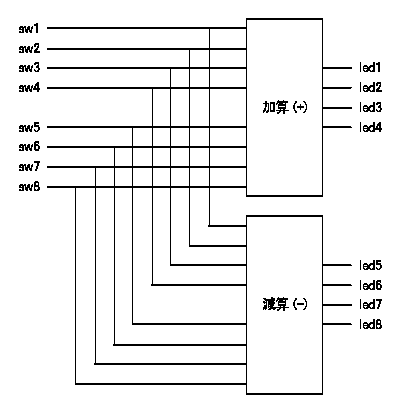
\includegraphics{figure07.eps}
\end{figure}


\section{5.4 条件分岐 when ~ else ~}
\label{05_try:when-else}

\subsection{5.4.1 演習}
\label{05_try:id7}
プロジェクト名 vhdl03

条件分岐の書き方の一つ、when ~ else ~ の例です。

\begin{Verbatim}[commandchars=\\\{\}]
\PYG{n}{l} \PYG{n}{i} \PYG{n}{b} \PYG{n}{r} \PYG{n}{a} \PYG{n}{r} \PYG{n}{y} \PYG{n}{i} \PYG{n}{e} \PYG{n}{e} \PYG{n}{e} \PYG{p}{;}
\PYG{k}{use} \PYG{n+nn}{i} \PYG{n}{e} \PYG{n}{e} \PYG{n}{e} \PYG{p}{.} \PYG{n}{s} \PYG{n}{t} \PYG{n}{d} \PYG{n}{l} \PYG{n}{o} \PYG{n}{g} \PYG{n}{i} \PYG{n}{c} \PYG{l+m+mi}{1} \PYG{l+m+mi}{1} \PYG{l+m+mi}{6} \PYG{l+m+mi}{4} \PYG{p}{.} \PYG{n}{a} \PYG{n}{l} \PYG{n}{l} \PYG{p}{;}
\PYG{k}{use} \PYG{n+nn}{i} \PYG{n}{e} \PYG{n}{e} \PYG{n}{e} \PYG{p}{.} \PYG{n}{s} \PYG{n}{t} \PYG{n}{d} \PYG{n}{l} \PYG{n}{o} \PYG{n}{g} \PYG{n}{i} \PYG{n}{c} \PYG{n}{a} \PYG{n}{r} \PYG{n}{i} \PYG{n}{t} \PYG{n}{h} \PYG{p}{.} \PYG{n}{a} \PYG{n}{l} \PYG{n}{l} \PYG{p}{;}
\PYG{k}{use} \PYG{n+nn}{i} \PYG{n}{e} \PYG{n}{e} \PYG{n}{e} \PYG{p}{.} \PYG{n}{s} \PYG{n}{t} \PYG{n}{d} \PYG{n}{l} \PYG{n}{o} \PYG{n}{g} \PYG{n}{i} \PYG{n}{c} \PYG{n}{u} \PYG{n}{n} \PYG{n}{s} \PYG{n}{i} \PYG{n}{g} \PYG{n}{n} \PYG{n}{e} \PYG{n}{d} \PYG{p}{.} \PYG{n}{a} \PYG{n}{l} \PYG{n}{l} \PYG{p}{;}
\PYG{n}{e} \PYG{n}{n} \PYG{n}{t} \PYG{n}{i} \PYG{n}{t} \PYG{n}{y} \PYG{n}{vhdl03} \PYG{n}{i} \PYG{n}{s}
\PYG{n}{por} \PYG{n}{t} \PYG{p}{(}
\PYG{n}{sw1} \PYG{o}{:} \PYG{k}{in} \PYG{n}{s} \PYG{n}{t} \PYG{n}{d} \PYG{n}{l} \PYG{n}{o} \PYG{n}{g} \PYG{n}{i} \PYG{n}{c} \PYG{p}{;}
\PYG{n}{sw2} \PYG{o}{:} \PYG{k}{in} \PYG{n}{s} \PYG{n}{t} \PYG{n}{d} \PYG{n}{l} \PYG{n}{o} \PYG{n}{g} \PYG{n}{i} \PYG{n}{c} \PYG{p}{;}
\PYG{n}{sw8} \PYG{o}{:} \PYG{k}{in} \PYG{n}{s} \PYG{n}{t} \PYG{n}{d} \PYG{n}{l} \PYG{n}{o} \PYG{n}{g} \PYG{n}{i} \PYG{n}{c} \PYG{p}{;}
\PYG{n}{l} \PYG{n}{ed1} \PYG{o}{:} \PYG{k}{out} \PYG{n}{s} \PYG{n}{t} \PYG{n}{d} \PYG{n}{l} \PYG{n}{o} \PYG{n}{g} \PYG{n}{i} \PYG{n}{c}
\PYG{p}{)} \PYG{p}{;}
\PYG{k}{end} \PYG{n+nc}{vhdl03} \PYG{p}{;}
\PYG{n}{a} \PYG{n}{r} \PYG{n}{c} \PYG{n}{h} \PYG{n}{i} \PYG{n}{t} \PYG{n}{e} \PYG{n}{c} \PYG{n}{t} \PYG{n}{u} \PYG{n}{r} \PYG{n}{e} \PYG{n}{beha} \PYG{n}{v} \PYG{n}{i} \PYG{n}{o} \PYG{n}{r} \PYG{n}{a} \PYG{n}{l} \PYG{n}{o} \PYG{n}{f} \PYG{n}{vhdl03} \PYG{n}{i} \PYG{n}{s}
\PYG{k}{begin}
\PYG{n}{l} \PYG{n}{ed1} \PYG{o}{\PYGZlt{}}\PYG{o}{=} \PYG{n}{sw2} \PYG{k}{when} \PYG{p}{(} \PYG{n}{sw8} \PYG{o}{=} \PYG{p}{\PYGZsq{}} \PYG{l+m+mi}{1} \PYG{p}{\PYGZsq{}} \PYG{p}{)}
\PYG{n}{e} \PYG{n}{l} \PYG{n}{s} \PYG{n}{e} \PYG{n}{sw1} \PYG{p}{;}
\PYG{k}{end} \PYG{n+nc}{beha} \PYG{n+nc}{v} \PYG{n+nc}{i} \PYG{n+nc}{o} \PYG{n+nc}{r} \PYG{n+nc}{a} \PYG{n+nc}{l} \PYG{p}{;}
\end{Verbatim}

sw8 をH レベルにしておくと、LED1 はsw2 の操作に従って点灯します。

sw8 がL レベルの場合は、LED1 はsw1 の操作に従って点灯します。

このコードから生成される回路のイメージは次の図の通りです。
\begin{figure}[htbp]
\centering

\includegraphics{figure08.eps}
\end{figure}

この記述ではいくつでも分岐させることができます。

\begin{Verbatim}[commandchars=\\\{\}]
\PYG{n}{ans} \PYG{o}{\PYGZlt{}}\PYG{o}{=} \PYG{n}{x1} \PYG{k}{when} \PYG{p}{(}\PYG{n}{y1} \PYG{o}{=} \PYG{l+s+sc}{\PYGZsq{}1\PYGZsq{}}\PYG{p}{)}
  \PYG{k}{else} \PYG{n}{x2} \PYG{k}{when} \PYG{p}{(}\PYG{n}{y2} \PYG{o}{=} \PYG{l+s+sc}{\PYGZsq{}1\PYGZsq{}}\PYG{p}{)}
  \PYG{k}{else} \PYG{n}{x3} \PYG{k}{when} \PYG{p}{(}\PYG{n}{y3} \PYG{o}{=} \PYG{l+s+sc}{\PYGZsq{}1\PYGZsq{}}\PYG{p}{)}
  \PYG{k}{else} \PYG{n}{x4} \PYG{k}{when} \PYG{p}{(}\PYG{n}{y4} \PYG{o}{=} \PYG{l+s+sc}{\PYGZsq{}1\PYGZsq{}}\PYG{p}{)}
  \PYG{k}{else} \PYG{n}{x5}\PYG{p}{;}
\end{Verbatim}

ただし、判定は記述した順番に行われます。この例でたとえばy1 ~ y4 全てが1 だった場合、y1 の条件が採用されます(プライオリティエンコーダ=選択肢に優先順位のあるセレクタ)。


\section{5.5 条件分岐 with ~ select ~ when ~}
\label{05_try:with-select-when}

\subsection{5.5.1 演習}
\label{05_try:id8}
プロジェクト名vhdl04

条件分岐の書き方の一つ、with ~ select ~ when ~ の例です。

\begin{Verbatim}[commandchars=\\\{\}]
\PYG{n}{l} \PYG{n}{i} \PYG{n}{b} \PYG{n}{r} \PYG{n}{a} \PYG{n}{r} \PYG{n}{y} \PYG{n}{i} \PYG{n}{e} \PYG{n}{e} \PYG{n}{e} \PYG{p}{;}
\PYG{k}{use} \PYG{n+nn}{i} \PYG{n}{e} \PYG{n}{e} \PYG{n}{e} \PYG{p}{.} \PYG{n}{s} \PYG{n}{t} \PYG{n}{d} \PYG{n}{l} \PYG{n}{o} \PYG{n}{g} \PYG{n}{i} \PYG{n}{c} \PYG{l+m+mi}{1} \PYG{l+m+mi}{1} \PYG{l+m+mi}{6} \PYG{l+m+mi}{4} \PYG{p}{.} \PYG{n}{a} \PYG{n}{l} \PYG{n}{l} \PYG{p}{;}
\PYG{k}{use} \PYG{n+nn}{i} \PYG{n}{e} \PYG{n}{e} \PYG{n}{e} \PYG{p}{.} \PYG{n}{s} \PYG{n}{t} \PYG{n}{d} \PYG{n}{l} \PYG{n}{o} \PYG{n}{g} \PYG{n}{i} \PYG{n}{c} \PYG{n}{a} \PYG{n}{r} \PYG{n}{i} \PYG{n}{t} \PYG{n}{h} \PYG{p}{.} \PYG{n}{a} \PYG{n}{l} \PYG{n}{l} \PYG{p}{;}
\PYG{k}{use} \PYG{n+nn}{i} \PYG{n}{e} \PYG{n}{e} \PYG{n}{e} \PYG{p}{.} \PYG{n}{s} \PYG{n}{t} \PYG{n}{d} \PYG{n}{l} \PYG{n}{o} \PYG{n}{g} \PYG{n}{i} \PYG{n}{c} \PYG{n}{u} \PYG{n}{n} \PYG{n}{s} \PYG{n}{i} \PYG{n}{g} \PYG{n}{n} \PYG{n}{e} \PYG{n}{d} \PYG{p}{.} \PYG{n}{a} \PYG{n}{l} \PYG{n}{l} \PYG{p}{;}
\PYG{n}{e} \PYG{n}{n} \PYG{n}{t} \PYG{n}{i} \PYG{n}{t} \PYG{n}{y} \PYG{n}{vhdl04} \PYG{n}{i} \PYG{n}{s}
\PYG{n}{por} \PYG{n}{t} \PYG{p}{(}
\PYG{n}{sw1} \PYG{o}{:} \PYG{k}{in} \PYG{n}{s} \PYG{n}{t} \PYG{n}{d} \PYG{n}{l} \PYG{n}{o} \PYG{n}{g} \PYG{n}{i} \PYG{n}{c} \PYG{p}{;}
\PYG{n}{sw2} \PYG{o}{:} \PYG{k}{in} \PYG{n}{s} \PYG{n}{t} \PYG{n}{d} \PYG{n}{l} \PYG{n}{o} \PYG{n}{g} \PYG{n}{i} \PYG{n}{c} \PYG{p}{;}
\PYG{n}{sw3} \PYG{o}{:} \PYG{k}{in} \PYG{n}{s} \PYG{n}{t} \PYG{n}{d} \PYG{n}{l} \PYG{n}{o} \PYG{n}{g} \PYG{n}{i} \PYG{n}{c} \PYG{p}{;}
\PYG{n}{sw7} \PYG{o}{:} \PYG{k}{in} \PYG{n}{s} \PYG{n}{t} \PYG{n}{d} \PYG{n}{l} \PYG{n}{o} \PYG{n}{g} \PYG{n}{i} \PYG{n}{c} \PYG{p}{;}
\PYG{n}{sw8} \PYG{o}{:} \PYG{k}{in} \PYG{n}{s} \PYG{n}{t} \PYG{n}{d} \PYG{n}{l} \PYG{n}{o} \PYG{n}{g} \PYG{n}{i} \PYG{n}{c} \PYG{p}{;}
\PYG{n}{l} \PYG{n}{ed1} \PYG{o}{:} \PYG{k}{out} \PYG{n}{s} \PYG{n}{t} \PYG{n}{d} \PYG{n}{l} \PYG{n}{o} \PYG{n}{g} \PYG{n}{i} \PYG{n}{c}
\PYG{p}{)} \PYG{p}{;}
\PYG{k}{end} \PYG{n+nc}{vhdl04} \PYG{p}{;}
\PYG{n}{a} \PYG{n}{r} \PYG{n}{c} \PYG{n}{h} \PYG{n}{i} \PYG{n}{t} \PYG{n}{e} \PYG{n}{c} \PYG{n}{t} \PYG{n}{u} \PYG{n}{r} \PYG{n}{e} \PYG{n}{beha} \PYG{n}{v} \PYG{n}{i} \PYG{n}{o} \PYG{n}{r} \PYG{n}{a} \PYG{n}{l} \PYG{n}{o} \PYG{n}{f} \PYG{n}{vhdl04} \PYG{n}{i} \PYG{n}{s}
\PYG{n}{s} \PYG{n}{i} \PYG{n}{g} \PYG{n}{n} \PYG{n}{a} \PYG{n}{l} \PYG{n}{sw} \PYG{o}{:} \PYG{n}{s} \PYG{n}{t} \PYG{n}{d} \PYG{n}{l} \PYG{n}{o} \PYG{n}{g} \PYG{n}{i} \PYG{n}{c} \PYG{n}{v} \PYG{n}{e} \PYG{n}{c} \PYG{n}{t} \PYG{n}{o} \PYG{n}{r} \PYG{p}{(}\PYG{l+m+mi}{1} \PYG{k}{downto} \PYG{l+m+mi}{0}\PYG{p}{)} \PYG{p}{;}
\PYG{k}{begin}
\PYG{n}{sw} \PYG{o}{\PYGZlt{}}\PYG{o}{=} \PYG{n}{sw8} \PYG{o}{\PYGZam{}} \PYG{n}{sw7} \PYG{p}{;}
\PYG{k}{with} \PYG{n}{sw} \PYG{n}{s} \PYG{n}{e} \PYG{n}{l} \PYG{n}{e} \PYG{n}{c} \PYG{n}{t} \PYG{n}{l} \PYG{n}{ed1} \PYG{o}{\PYGZlt{}}\PYG{o}{=} \PYG{n}{sw3} \PYG{k}{when} \PYG{l+s}{\PYGZdq{}11\PYGZdq{}} \PYG{p}{,}
\PYG{n}{sw2} \PYG{k}{when} \PYG{l+s}{\PYGZdq{}10\PYGZdq{}} \PYG{p}{,}
\PYG{n}{sw1} \PYG{k}{when} \PYG{l+s}{\PYGZdq{}01\PYGZdq{}} \PYG{p}{,}
\PYG{p}{\PYGZsq{}}\PYG{l+m+mi}{0} \PYG{p}{\PYGZsq{}} \PYG{k}{when} \PYG{n}{o} \PYG{n}{the} \PYG{n}{r} \PYG{n}{s} \PYG{p}{;}
\PYG{k}{end} \PYG{n+nc}{beha} \PYG{n+nc}{v} \PYG{n+nc}{i} \PYG{n+nc}{o} \PYG{n+nc}{r} \PYG{n+nc}{a} \PYG{n+nc}{l} \PYG{p}{;}
\end{Verbatim}

sw7 とsw8 の設定により、LED の点滅を制御できるスイッチを切り替えられる回路です。

このコードから生成される回路のイメージは次の通りです。
\begin{figure}[htbp]
\centering

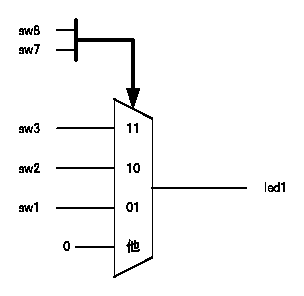
\includegraphics{figure09.eps}
\end{figure}

中央のブロックはセレクタで、上から入力される値がブロック中の値と一致すると、その箇所の信号が出力されます。


\section{5.6 process 文}
\label{05_try:process}
AND、OR、NOT などの組み合わせ回路や単純な条件分岐であればこれまでの内容で対応できますが、フリップフロップなどを組み合わせた順序回路を記述するには、process文を使用します。

ヒント

フリップフロップ専用の記述ではありませんが、フリップフロップを使用する箇所のみ process 文を使うようにしていると、慣れていないうちはトラブルを避けやすくなります。

基本的な構成は以下の通りです。

\begin{Verbatim}[commandchars=\\\{\}]
LABEL: process (SENSITIVITY\PYGZhy{}LIST)
begin
  ~ EXPRESSION ~
end process;
\end{Verbatim}

ラベル(LABEL) を付加するかどうかは任意ですが、識別のために固有の名前をつけておくのがよいでしょう。

センシティビティリスト(SENSITIVITY-LIST) は、このprocess 文を動作させるトリガになる信号のリストを記述します。

信号名はカンマで区切ります。

式(EXPRESSION) の部分には実際の動作を記述します。ただし条件分岐は、これまでのwhen ~ else ~ やwith ~ select ~ when ~ は使用できません。後ほどでてくるif 文やcase 文を使用します(逆にif  文やcase 文はprocess 文の外では使用できません)。


\begin{threeparttable}
\capstart\caption{組み合わせ}\label{05_try:id31}
\begin{tabulary}{\linewidth}{|L|L|L|L|L|}
\hline
\textsf{\relax 
process 文の
} & \textsf{\relax 
when ~ else ~
} & \textsf{\relax 
with ~ select ~ when ~
} & \textsf{\relax 
if ~ elsif ~ endif
} & \textsf{\relax 
case ~ end case
}\\
\hline
外
 & 
○
 & 
○
 & 
×
 & 
×
\\
\hline
中
 & 
×
 & 
×
 & 
○
 & 
○
\\
\hline\end{tabulary}

\end{threeparttable}



\section{5.7 フリップフロップの基本と if 文}
\label{05_try:if}
フリップフロップは主にD 型、SR 型、JK 型、T 型があります。これらをVHDL で記述するときは一般にprocess 文を使用します。

フリップフロップのリセットが非同期式の場合、D フリップフロップは以下のように記述します。

\begin{Verbatim}[commandchars=\\\{\}]
\PYG{n}{D\PYGZus{}FF}\PYG{o}{:} \PYG{k}{process} \PYG{p}{(}\PYG{n}{reset}\PYG{p}{,} \PYG{n}{clock}\PYG{p}{)}
\PYG{k}{begin}
  \PYG{k}{if} \PYG{p}{(}\PYG{n}{reset} \PYG{o}{=} \PYG{l+s+sc}{\PYGZsq{}1\PYGZsq{}}\PYG{p}{)} \PYG{k}{then}
    \PYG{n}{q} \PYG{o}{\PYGZlt{}}\PYG{o}{=} \PYG{l+s+sc}{\PYGZsq{}0\PYGZsq{}}\PYG{p}{;}
  \PYG{k}{elsif} \PYG{p}{(}\PYG{n}{clock}\PYG{n+na}{\PYGZsq{}event} \PYG{k}{and} \PYG{n}{clock} \PYG{o}{=} \PYG{l+s+sc}{\PYGZsq{}1\PYGZsq{}}\PYG{p}{)} \PYG{k}{then}
    \PYG{n}{q} \PYG{o}{\PYGZlt{}}\PYG{o}{=} \PYG{n}{d}\PYG{p}{;}
  \PYG{k}{end} \PYG{k}{if}\PYG{p}{;}
\PYG{k}{end} \PYG{k}{process}\PYG{p}{;}
\end{Verbatim}

この例では、すべての信号は std\_logic で定義されているとします。

入力データは信号は d 、出力データ信号は q としています。

reset に H レベルの信号を与えるとリセット動作として、q をL レベルにセットしています。

クロック信号 clock が H へ変化すると、q へ d を代入します。
\begin{figure}[htbp]
\centering

\includegraphics{figure12.eps}
\end{figure}

動作例を以下に示します。
\begin{figure}[htbp]
\centering

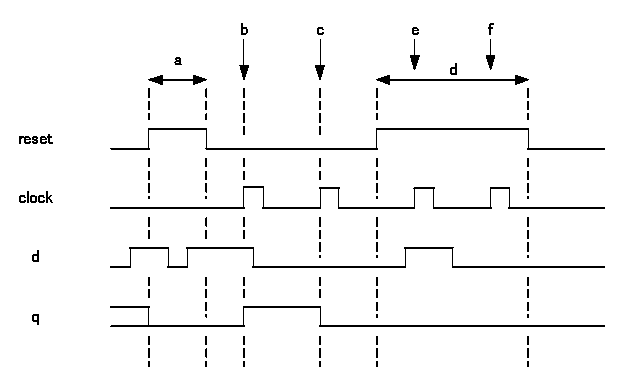
\includegraphics{figure10.eps}
\end{figure}

a の期間では reset = `1' が成り立つので q \textless{}= `0' が実行され続けます。

b のタイミングでは clock'event and clock = `1' が成り立ちます。これは、clock が変化したこと(clock'event)と clock = `1' の組み合わせで、clock が 0 から 1 に変化したときに成り立つ、という記述の仕方です。このとき q \textless{}= d が実行されます。d が 1 なので最終的には q は 1 になります。

c のタイミングも b のタイミング同様、clock が 0 から 1 に変化したことが成り立っています。q には d の値 0 が代入されます。

d の期間では e や f のタイミングで clock'event が成り立っていますが、if 文(後述)で reset = `1' が先に記述されているため、e 、f は無視され、q には 0 が出力され続けます。

ちなみに FPGA が起動したとき、フリップフロップの値が H 、L どちらになっているかは決まっていません。そのため図で q はリセットがかかるまではどちらの値かわかりません(不定)。


\subsection{5.7.1 同期、非同期}
\label{05_try:id9}
「非同期」動作は、クロックによらず動作する箇所、「同期」動作はクロックの変化点に合わせて動作することを示しています。

先ほどのサンプルでは、リセットは非同期動作(特にこの場合は「非同期リセット」とも呼ばれる)、データの保持は同期動作としています。

\begin{notice}{note}{注釈:}
データをクロックに同期して保持するものを一般にフリップフロップ、同期せずに保持するものをラッチと呼びます。

これは「ディジタルコンピューティングシステム」p54 に書かれていることと逆ですが、会社などの組織毎に異なる場合があるので注意が必要です。
\end{notice}

\begin{notice}{warning}{警告:}
FPGA に実装する回路において、一般にラッチは使用するべきではないとされています。

フリップフロップを使った方が動作が予測しやすいため、デバイス自体にフリップフロップが組み込まれています。それに対しラッチは大規模回路では動作の予測が難しく、バグの元になりやすいため、です。

慣れないうちは、できる限りすべてのフリップフロップは同じクロックで動作するようにし、動作を始める前にはすべて非同期リセットを行うように組むと失敗が少なくなります。
\end{notice}

\begin{notice}{note}{注釈:}
「ディジタル回路」は信号レベル(縦軸)を離散的に扱います。「同期回路」は時間軸を離散的に扱うための手法と考えられます。「非同期回路」は時間軸に不確定な要因を持つことになるため、動作の安定性に影響します。

この授業の実習では、その実習で使用するすべてのフリップフロップは同じクロックで動作させるようにします。

これらを守るためには、上のD フリップフロップの例のようなセンシティビティリスト(信号名は回路に合わせる)、if 文の構成(非同期リセットとクロックの動作しかなく、それ以上はそのif 、elsif の中に書き足していく)を基本にしていきます。
\end{notice}


\subsection{5.7.2 if 文}
\label{05_try:id10}
条件分岐の基本的なもので、基本的な形は以下の通りです。

\begin{Verbatim}[commandchars=\\\{\}]
if (CONDITION) then
  ~ EXPRESSION ~
end if;
\end{Verbatim}

条件(CONDITION) が真であれば、処理(EXPRESSION) が実行されます。
複数の条件ごとに処理を分ける場合は以下のようになります。

\begin{Verbatim}[commandchars=\\\{\}]
if (CONDITION\PYGZus{}A) then
  ~ EXPRESSION\PYGZus{}A ~
elsif (CONDITION\PYGZus{}B) then
  ~ EXPRESSION\PYGZus{}B ~
elsif (CONDITION\PYGZus{}C) then
  ~ EXPRESSION\PYGZus{}C ~
else
  ~ EXPRESSION\PYGZus{}OTHER ~
end if;
\end{Verbatim}

条件A (CONDITION-A) が真であれば処理A (EXPRESSION-A) を実行、それ以外で条件B (CONDITION-B) が真であれば処理B (EXPRESSION-B) 、それ以外で条件C (CONDITION-C) が真であれば処理C (EXPRESSION-C)、それ以外ではその他の処理(EXPRESSION-OTHERS) を実行します。

\begin{notice}{note}{注釈:}
一般のプログラミング言語と異なり、「else if」ではなく「elsif」と書きます。
\end{notice}

条件の書き方は、たとえば一致判定では

\begin{Verbatim}[commandchars=\\\{\}]
\PYG{n}{reset} \PYG{o}{=} \PYG{l+s+sc}{\PYGZsq{}1\PYGZsq{}}
\end{Verbatim}

数値の大小の比較では、

\begin{Verbatim}[commandchars=\\\{\}]
\PYG{n}{count} \PYG{o}{\PYGZgt{}}\PYG{o}{=} \PYG{l+s}{\PYGZdq{}1010\PYGZdq{}}
\end{Verbatim}

となります。

条件は複数組み合わせることができ、そのときは and 、or 、not も使用できます。

たとえば

\begin{Verbatim}[commandchars=\\\{\}]
\PYG{n}{a} \PYG{o}{=} \PYG{l+s+sc}{\PYGZsq{}1\PYGZsq{}} \PYG{k}{and} \PYG{n}{b} \PYG{o}{=} \PYG{l+s+sc}{\PYGZsq{}0\PYGZsq{}}
\end{Verbatim}

とすれば、2つの条件が満たされた場合、と判定されます。
クロックの変化点での動作、つまり同期動作について括る場合の条件は、

\begin{Verbatim}[commandchars=\\\{\}]
\PYG{n}{clock}\PYG{n+na}{\PYGZsq{}event} \PYG{k}{and} \PYG{n}{clock} \PYG{o}{=} \PYG{l+s+sc}{\PYGZsq{}1\PYGZsq{}}
\end{Verbatim}

が一般的となります。これは clock の変化点と、clock が H という2つの条件のANDとなります。

\begin{notice}{note}{注釈:}
上記のような、クロックの変化点での動作の記述は、一つの if 文で複数書いても文法上は問題ありませんが、実際のデバイス上でそのような動作は行うことができません。
\end{notice}

一般に process 文の最初の if 文の構成は最大で

\begin{Verbatim}[commandchars=\\\{\}]
process (set, reset, clock)
begin
  if (reset = \PYGZsq{}1\PYGZsq{}) then
    ~
  elsif (set = \PYGZsq{}1\PYGZsq{}) then
    ~
  elsif (clock\PYGZsq{}event and clock = \PYGZsq{}1\PYGZsq{}) then
    ~
  end if ;
end process;
\end{Verbatim}

となります。

リセット時、セット(プリセット)時、その他通常動作時を同じレベルで設定しています。

以下の書き方は許容されますが、理解できていないうちは行うべきではありません。

\begin{Verbatim}[commandchars=\\\{\}]
process (clock)
begin
  if (clock\PYGZsq{}event and clock = \PYGZsq{}1\PYGZsq{}) then
    ~
  end if;
end process;
process (clock)
begin
  if (clock\PYGZsq{}event and clock = \PYGZsq{}0\PYGZsq{}) then
    ~
  end if;
end process;
\end{Verbatim}

同じクロックで動作する書き方ですが、1 = クロックの立ち上がりと 0 = クロックの立ち下がりが混在しています。この2つの process 文の間でデータのやりとりがあるとき、デバイス上での動作条件が厳しくなります。

以下の書き方は実機には基本的には組み込めません。

\begin{Verbatim}[commandchars=\\\{\}]
process (clock)
begin
  if (clock\PYGZsq{}event and clock = \PYGZsq{}1\PYGZsq{}) then
    ~
  elsif (clock\PYGZsq{}event and clock = \PYGZsq{}0\PYGZsq{}) then
    ~
  end if;
end process;
\end{Verbatim}

同じ process 文内で、同じクロックの 1 = クロックの立ち上がりと 0 = クロックの立ち下がりが混在しています。同じ signal に対してこのような動作は指示できません。それぞれの処理に異なる signal を入れれば組み込むことはできますが、一つ前の例と同様使うべきではありません。


\subsection{5.7.3 マルチソース}
\label{05_try:id11}
HDL では、基本的に全ての行が、常に「同時」に動作していると考える必要があります。この点が、ソースコードを逐次解釈していくソフトウェアと大きく異なる点です。

これにより、signal や port への値の代入の仕方に制限があります。

\begin{Verbatim}[commandchars=\\\{\}]
\PYG{k}{architecture} \PYG{n+nc}{rtl} \PYG{k}{of} \PYG{n+nc}{test} \PYG{k}{is}
  \PYG{k}{signal} \PYG{n}{a} \PYG{o}{:} \PYG{k+kt}{std\PYGZus{}logic}\PYG{p}{;}
\PYG{k}{begin}
  \PYG{n}{a} \PYG{o}{\PYGZlt{}}\PYG{o}{=} \PYG{l+s+sc}{\PYGZsq{}0\PYGZsq{}}\PYG{p}{;}
  \PYG{n}{a} \PYG{o}{\PYGZlt{}}\PYG{o}{=} \PYG{l+s+sc}{\PYGZsq{}1\PYGZsq{}}\PYG{p}{;}
\PYG{k}{end} \PYG{n+nc}{rtl}\PYG{p}{;}
\end{Verbatim}

ソフトウェアであればこの場合、a に 0 が代入された後でさらに a に 1 が代入されます。
しかし HDL の場合、0 と 1 の代入は同時に行おうとし、論理合成の段階でエラーとなります(エラーメッセージには multi source という言葉が含まれます)。

\begin{Verbatim}[commandchars=\\\{\}]
\PYG{k}{entity} \PYG{n+nc}{x} \PYG{k}{is}
  \PYG{k}{port} \PYG{p}{(}
    \PYG{n}{d1} \PYG{o}{:} \PYG{k}{in} \PYG{k+kt}{std\PYGZus{}logic}\PYG{p}{;}
    \PYG{n}{d2} \PYG{o}{:} \PYG{k}{in} \PYG{k+kt}{std\PYGZus{}logic}\PYG{p}{;}
    \PYG{n}{clk} \PYG{o}{:} \PYG{k}{in} \PYG{k+kt}{std\PYGZus{}logic}\PYG{p}{;}
    \PYG{n}{q} \PYG{o}{:} \PYG{k}{out} \PYG{k+kt}{std\PYGZus{}logic}
  \PYG{p}{)} \PYG{p}{;}
\PYG{k}{end} \PYG{n+nc}{x}\PYG{p}{;}

\PYG{k}{architecture} \PYG{n+nc}{rtl} \PYG{k}{of} \PYG{n+nc}{x} \PYG{k}{is}
  \PYG{k}{signal} \PYG{n}{a} \PYG{o}{:} \PYG{k+kt}{std\PYGZus{}logic}\PYG{p}{;}
\PYG{k}{begin}
  \PYG{n}{a\PYGZus{}proc} \PYG{o}{:} \PYG{k}{process} \PYG{p}{(}\PYG{n}{clk}\PYG{p}{)}
  \PYG{k}{begin}
    \PYG{k}{if} \PYG{p}{(}\PYG{n}{clk}\PYG{n+na}{\PYGZsq{}event} \PYG{k}{and} \PYG{n}{clk} \PYG{o}{=} \PYG{l+s+sc}{\PYGZsq{}1\PYGZsq{}}\PYG{p}{)} \PYG{k}{then}
      \PYG{n}{a} \PYG{o}{\PYGZlt{}}\PYG{o}{=} \PYG{n}{d1}\PYG{p}{;}
    \PYG{k}{end} \PYG{k}{if}\PYG{p}{;}
  \PYG{k}{end} \PYG{k}{process}\PYG{p}{;}

  \PYG{n}{b\PYGZus{}proc} \PYG{o}{:} \PYG{k}{process} \PYG{p}{(}\PYG{n}{clk}\PYG{p}{)}
  \PYG{k}{begin}
    \PYG{k}{if} \PYG{p}{(}\PYG{n}{clk}\PYG{n+na}{\PYGZsq{}event} \PYG{k}{and} \PYG{n}{clk} \PYG{o}{=} \PYG{l+s+sc}{\PYGZsq{}1\PYGZsq{}}\PYG{p}{)} \PYG{k}{then}
      \PYG{n}{a} \PYG{o}{\PYGZlt{}}\PYG{o}{=} \PYG{n}{d2}\PYG{p}{;}
    \PYG{k}{end} \PYG{k}{if}\PYG{p}{;}
  \PYG{k}{end} \PYG{k}{process}\PYG{p}{;}

  \PYG{n}{q} \PYG{o}{\PYGZlt{}}\PYG{o}{=} \PYG{n}{a}\PYG{p}{;}

\PYG{k}{end} \PYG{n+nc}{rtl}\PYG{p}{;}
\end{Verbatim}

別々の process 文で動作させていても、同じ signal に代入しようとしているため、両方の条件が必ず衝突しない書き方出ない限り論理合成でエラーになります(そしてそのように書いたとしても不具合の修正なので書き換えているうちに条件が崩れ multi source のエラーになりやすいです)。

\begin{Verbatim}[commandchars=\\\{\}]
\PYG{k}{entity} \PYG{n+nc}{x} \PYG{k}{is}
  \PYG{k}{port} \PYG{p}{(}
    \PYG{n}{d1} \PYG{o}{:} \PYG{k}{in} \PYG{k+kt}{std\PYGZus{}logic}\PYG{p}{;}
    \PYG{n}{d2} \PYG{o}{:} \PYG{k}{in} \PYG{k+kt}{std\PYGZus{}logic}\PYG{p}{;}
    \PYG{n}{clk} \PYG{o}{:} \PYG{k}{in} \PYG{k+kt}{std\PYGZus{}logic}\PYG{p}{;}
    \PYG{n}{q} \PYG{o}{:} \PYG{k}{out} \PYG{k+kt}{std\PYGZus{}logic}
  \PYG{p}{)} \PYG{p}{;}
\PYG{k}{end} \PYG{n+nc}{x} \PYG{p}{;}

\PYG{k}{architecture} \PYG{n+nc}{rtl} \PYG{k}{of} \PYG{n+nc}{x} \PYG{k}{is}
  \PYG{k}{signal} \PYG{n}{a} \PYG{o}{:} \PYG{k+kt}{std\PYGZus{}logic}\PYG{p}{;}
\PYG{k}{begin}
  \PYG{n}{a} \PYG{n}{proc} \PYG{o}{:} \PYG{k}{process} \PYG{p}{(}\PYG{n}{clk}\PYG{p}{)}
  \PYG{k}{begin}
    \PYG{k}{if} \PYG{p}{(}\PYG{n}{clk}\PYG{n+na}{\PYGZsq{}event} \PYG{k}{and} \PYG{n}{clk} \PYG{o}{=} \PYG{l+s+sc}{\PYGZsq{}1\PYGZsq{}}\PYG{p}{)} \PYG{k}{then}
      \PYG{n}{a} \PYG{o}{\PYGZlt{}}\PYG{o}{=} \PYG{n}{d1}\PYG{p}{;}
    \PYG{k}{end} \PYG{k}{if}\PYG{p}{;}
  \PYG{k}{end} \PYG{k}{process}\PYG{p}{;}

  \PYG{n}{a} \PYG{o}{\PYGZlt{}}\PYG{o}{=} \PYG{n}{d2}\PYG{p}{;}
  \PYG{n}{q} \PYG{o}{\PYGZlt{}}\PYG{o}{=} \PYG{n}{a}\PYG{p}{;}

\PYG{k}{end} \PYG{n+nc}{rtl}\PYG{p}{;}
\end{Verbatim}

このような process 文での順序回路と、通常の組み合わせ回路でも同様です。


\subsection{5.7.4 process 文、if 文によるフリップフロップの記述のお約束}
\label{05_try:process-if}
この教科書ではこの先順序回路を多く使用します。その際、後々のトラブルを避けるため、以下のような書き方を避けることをおすすめします。

\begin{Verbatim}[commandchars=\\\{\}]
process (reset, clock, a, b)
begin
  if (reset = \PYGZsq{}1\PYGZsq{}) then
    ~ RESET\PYGZhy{}PROCEDURE ~
  elsif (clock\PYGZsq{}event and clock = \PYGZsq{}1\PYGZsq{} and a = \PYGZsq{}1\PYGZsq{}) then
    ~ PROCEDURE\PYGZhy{}A ~
  elsif (clock\PYGZsq{}event and clock = \PYGZsq{}1\PYGZsq{} and b = \PYGZsq{}1\PYGZsq{}) then
    ~ PROCEDURE\PYGZhy{}B ~
  end if;
end process;
\end{Verbatim}

どうやら、リセット処理(RESET-PROCEDURE)、クロックに同期した上で a が 1 の時の処理(PROCEDURE-A)、クロックに同期した上で b が 1 の時の処理(PROCEDURE-B)を行いたいらしい。

このような場合は以下のように、クロックによる動作と論理を分離して記述すると良いでしょう。

\begin{Verbatim}[commandchars=\\\{\}]
process (reset , clock)
begin
  if (reset = \PYGZsq{}1\PYGZsq{}) then
    ~ RESET PROCEDURE ~
  elsif (clock\PYGZsq{}event and clock = \PYGZsq{}1\PYGZsq{}) then
    if (a = \PYGZsq{}1\PYGZsq{}) then
      ~ PROCEDURE A ~
    elsif (b = \PYGZsq{}1\PYGZsq{}) then
      ~ PROCEDURE B ~
    end if;
  end if;
end process ;
\end{Verbatim}

クロックの条件に追加で書いていると、この授業のレベルではその箇所でミスをしやすくなります。

またクロックの条件と分離することで、他へのコピー&ペーストでのミスも減ります。

このほか、以下の箇所で代入を行っても、意図した動作にならない可能性が高いです。

\begin{Verbatim}[commandchars=\\\{\}]
process (reset , clock)
begin
  if (reset = \PYGZsq{}1\PYGZsq{}) then
    ~ RESET PROCEDURE ~
  elsif (clock\PYGZsq{}event and clock = \PYGZsq{}1\PYGZsq{}) then
    ~ MAIN PROCEDURE ~
  end if;
  a \PYGZlt{}= b;
end process;
\end{Verbatim}

a へ b を代入していますが、この位置ではセンシティビティリストに入る reset と clock の条件を無視した位置にあるため、どのような動作になるか保証できません。

process 文の外か、if 文の中に入れましょう。


\subsection{5.7.5 演習}
\label{05_try:id12}
プロジェクト名 vhdl05

D フリップフロップを作る

\begin{Verbatim}[commandchars=\\\{\}]
\PYG{k}{library} \PYG{n+nn}{ieee} \PYG{p}{;}
\PYG{k}{use} \PYG{n+nn}{ieee.std\PYGZus{}logic\PYGZus{}1164.all}\PYG{p}{;}
\PYG{k}{use} \PYG{n+nn}{ieee.std\PYGZus{}logic\PYGZus{}arith.all}\PYG{p}{;}
\PYG{k}{use} \PYG{n+nn}{ieee.std\PYGZus{}logic\PYGZus{}unsigned.all}\PYG{p}{;}

\PYG{k}{entity} \PYG{n+nc}{vhdl05} \PYG{k}{is}
  \PYG{k}{port} \PYG{p}{(}
    \PYG{n}{sw1} \PYG{o}{:} \PYG{k}{in} \PYG{k+kt}{std\PYGZus{}logic} \PYG{p}{;} \PYG{c+c1}{\PYGZhy{}\PYGZhy{} data}
    \PYG{n}{sw2} \PYG{o}{:} \PYG{k}{in} \PYG{k+kt}{std\PYGZus{}logic} \PYG{p}{;} \PYG{c+c1}{\PYGZhy{}\PYGZhy{} clock}
    \PYG{n}{sw3} \PYG{o}{:} \PYG{k}{in} \PYG{k+kt}{std\PYGZus{}logic} \PYG{p}{;} \PYG{c+c1}{\PYGZhy{}\PYGZhy{} reset}
    \PYG{n}{led1} \PYG{o}{:} \PYG{k}{out} \PYG{k+kt}{std\PYGZus{}logic}
  \PYG{p}{)}\PYG{p}{;}
\PYG{k}{end} \PYG{n+nc}{vhdl05}\PYG{p}{;}

\PYG{k}{architecture} \PYG{n+nc}{rtl} \PYG{k}{of} \PYG{n+nc}{vhdl05} \PYG{k}{is}
  \PYG{k}{signal} \PYG{n}{d} \PYG{o}{:} \PYG{k+kt}{std\PYGZus{}logic}\PYG{p}{;}
\PYG{k}{begin}
  \PYG{n}{dff} \PYG{o}{:} \PYG{k}{process} \PYG{p}{(}\PYG{n}{sw2}\PYG{p}{,} \PYG{n}{sw3}\PYG{p}{)}
  \PYG{k}{begin}
    \PYG{k}{if} \PYG{p}{(}\PYG{n}{sw3} \PYG{o}{=} \PYG{l+s+sc}{\PYGZsq{}1\PYGZsq{}}\PYG{p}{)} \PYG{k}{then}
      \PYG{n}{d} \PYG{o}{\PYGZlt{}}\PYG{o}{=} \PYG{l+s+sc}{\PYGZsq{}0\PYGZsq{}}\PYG{p}{;}
    \PYG{k}{elsif} \PYG{p}{(}\PYG{n}{sw2}\PYG{n+na}{\PYGZsq{}event} \PYG{k}{and} \PYG{n}{sw2} \PYG{o}{=} \PYG{l+s+sc}{\PYGZsq{}1\PYGZsq{}}\PYG{p}{)} \PYG{k}{then}
      \PYG{n}{d} \PYG{o}{\PYGZlt{}}\PYG{o}{=} \PYG{n}{sw1}\PYG{p}{;}
    \PYG{k}{end} \PYG{k}{if}\PYG{p}{;}
  \PYG{k}{end} \PYG{k}{process}\PYG{p}{;}

  \PYG{n}{led1} \PYG{o}{\PYGZlt{}}\PYG{o}{=} \PYG{n}{d}\PYG{p}{;}
\PYG{k}{end} \PYG{n+nc}{rtl}\PYG{p}{;}
\end{Verbatim}

ヒント

``--``(マイナス2個)以降は改行までコメントとして無視されます。

この例では、sw1 をデータ入力、sw2 をクロック、sw3 をリセットとして使用しています。

シグナル d を D フリップフロップの実態という意味で定義しています。

sw3 を H にすると、フリップフロップをリセットします。

sw2 が H に変化したタイミング(立ち上がりエッジ)で、sw1 の内容を d へ代入します。そのほかのタイミングでは sw1 の変化の影響を受けません。

process 文内の処理は sw2 と sw3 の変化でしか行われないため、センシティビティリストには sw2 と sw3 しか書いていません。

led1 には d の内容を出力しています。
\begin{figure}[htbp]
\centering

\includegraphics{figure13.eps}
\end{figure}

動作確認
\begin{enumerate}
\item {} 
sw1、sw2、sw3 をすべてOFF にする。

\item {} 
まず sw3 を ON \(\rightarrow\) OFF して、リセットする。

\item {} 
sw2 を ON \(\rightarrow\) OFF して、led1 が変化しないことを確認する。(入力データ sw1 が OFF なので、OFF のデータを改めてサンプルするだけ)

\item {} 
sw1 を ON にする。

\item {} 
sw2 を ON \(\rightarrow\) OFF して、 led1 が変化することを確認する。

\item {} 
sw1 を OFF にしても led1 が変化しないことを確認する。

\item {} 
sw2 を ON \(\rightarrow\) OFF して、 led1 が変化することを確認する。

\end{enumerate}


\subsection{5.7.6 課題}
\label{05_try:id13}
プロジェクト名 vhdl06

下記のソースコードに追記して、JK フリップフロップを作れ

\begin{Verbatim}[commandchars=\\\{\}]
\PYG{k}{library} \PYG{n+nn}{ieee}\PYG{p}{;}
\PYG{k}{use} \PYG{n+nn}{ieee.std\PYGZus{}logic\PYGZus{}1164.all}\PYG{p}{;}
\PYG{k}{use} \PYG{n+nn}{ieee.std\PYGZus{}logic\PYGZus{}arith.all}\PYG{p}{;}
\PYG{k}{use} \PYG{n+nn}{ieee.std\PYGZus{}logic\PYGZus{}unsigned.all}\PYG{p}{;}

\PYG{k}{entity} \PYG{n+nc}{vhdl06} \PYG{k}{is}
  \PYG{k}{port} \PYG{p}{(}
    \PYG{n}{sw1} \PYG{o}{:} \PYG{k}{in} \PYG{k+kt}{std\PYGZus{}logic}\PYG{p}{;} \PYG{c+c1}{\PYGZhy{}\PYGZhy{} J}
    \PYG{n}{sw2} \PYG{o}{:} \PYG{k}{in} \PYG{k+kt}{std\PYGZus{}logic}\PYG{p}{;} \PYG{c+c1}{\PYGZhy{}\PYGZhy{} clock}
    \PYG{n}{sw3} \PYG{o}{:} \PYG{k}{in} \PYG{k+kt}{std\PYGZus{}logic}\PYG{p}{;} \PYG{c+c1}{\PYGZhy{}\PYGZhy{} K}
    \PYG{n}{sw4} \PYG{o}{:} \PYG{k}{in} \PYG{k+kt}{std\PYGZus{}logic}\PYG{p}{;} \PYG{c+c1}{\PYGZhy{}\PYGZhy{} reset}
    \PYG{n}{led1} \PYG{o}{:} \PYG{k}{out} \PYG{k+kt}{std\PYGZus{}logic}
  \PYG{p}{)}\PYG{p}{;}
\PYG{k}{end} \PYG{n+nc}{vhdl06}\PYG{p}{;}

\PYG{k}{architecture} \PYG{n+nc}{rtl} \PYG{k}{of} \PYG{n+nc}{vhdl06} \PYG{k}{is}
  \PYG{k}{signal} \PYG{n}{jk} \PYG{o}{:} \PYG{k+kt}{std\PYGZus{}logic}\PYG{p}{;}
\PYG{k}{begin}
  \PYG{n}{jkff\PYGZus{}proc} \PYG{o}{:} \PYG{k}{process} \PYG{p}{(}\PYG{n}{sw4}\PYG{p}{,} \PYG{n}{sw2}\PYG{p}{)}
  \PYG{k}{begin}
    \PYG{k}{if} \PYG{p}{(}\PYG{n}{sw4} \PYG{o}{=} \PYG{l+s+sc}{\PYGZsq{}1\PYGZsq{}}\PYG{p}{)} \PYG{k}{then}
       \PYG{c+c1}{\PYGZhy{}\PYGZhy{} put code below \PYGZhy{}\PYGZhy{}}

       \PYG{c+c1}{\PYGZhy{}\PYGZhy{} put code above \PYGZhy{}\PYGZhy{}}
    \PYG{k}{elsif} \PYG{p}{(}\PYG{n}{sw2}\PYG{n+na}{\PYGZsq{}event} \PYG{k}{and} \PYG{n}{sw2} \PYG{o}{=} \PYG{l+s+sc}{\PYGZsq{}1\PYGZsq{}}\PYG{p}{)} \PYG{k}{then}
       \PYG{c+c1}{\PYGZhy{}\PYGZhy{} put code below \PYGZhy{}\PYGZhy{}}

       \PYG{c+c1}{\PYGZhy{}\PYGZhy{} put code above \PYGZhy{}\PYGZhy{}}
    \PYG{k}{end} \PYG{k}{if}\PYG{p}{;}
  \PYG{k}{end} \PYG{k}{process}\PYG{p}{;}

  \PYG{n}{led1} \PYG{o}{\PYGZlt{}}\PYG{o}{=} \PYG{n}{jk}\PYG{p}{;}
\PYG{k}{end} \PYG{n+nc}{rtl}\PYG{p}{;}
\end{Verbatim}

2箇所の''put code below'' から''put code above'' の間にコードを書いてください。

ソースコード中で指定しているようなスイッチのアサインで、JK フリップフロップを作成してください。
\begin{figure}[htbp]
\centering

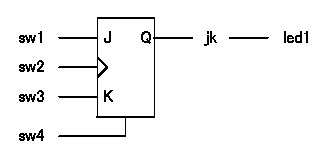
\includegraphics{figure14.eps}
\end{figure}


\begin{threeparttable}
\capstart\caption{真理値表}\label{05_try:id32}
\begin{tabulary}{\linewidth}{|L|L|L|L|}
\hline
\textsf{\relax 
sw2 (clock)
} & \textsf{\relax 
sw1(J)
} & \textsf{\relax 
sw3(K)
} & \textsf{\relax 
led1(Q \(\rightarrow\) jk)
}\\
\hline
↑以外
 & 
X
 & 
X
 & 
維持
\\
\hline
↑
 & 
0
 & 
0
 & 
維持
\\
\hline
↑
 & 
1
 & 
0
 & 
1
\\
\hline
↑
 & 
0
 & 
1
 & 
0
\\
\hline
↑
 & 
1
 & 
1
 & 
反転
\\
\hline\end{tabulary}

\end{threeparttable}


動作確認は以下の通り行います。
\begin{enumerate}
\item {} 
sw1 ~ sw4 を OFF にする。

\item {} 
sw4 を ON \(\rightarrow\) OFF として、リセットする(led1 が点灯する)。

\item {} 
sw1 を ON \(\rightarrow\) OFF として、led1 が変化しないことを確認する(J だけ動かしている)。

\item {} 
sw3 を ON \(\rightarrow\) OFF として、led1 が変化しないことを確認する(K だけ動かしている)。

\item {} 
sw1 を ON にし、sw2 を ON \(\rightarrow\) OFF として、led1 が消灯することを確認する。

\item {} 
sw1 を OFF にし、sw2 を ON \(\rightarrow\) OFF としても、led1 が消灯したままであることを確認する。

\item {} 
sw3 を ON にし、sw2 を ON \(\rightarrow\) OFF として、led1 が点灯することを確認する。

\item {} 
sw3 を OFF にし、sw2 を ON \(\rightarrow\) OFF としても、led1 が点灯したままとなることを確認する。

\item {} 
sw1 、sw3 を ON にし、sw2 を ON \(\rightarrow\) OFF として、led1 が消灯することを確認する(注記参照)。

\item {} 
sw1 、sw3 を ON にしたままで、sw2 を ON \(\rightarrow\) OFF として、led1 が点灯することを確認する(注記参照)。

\end{enumerate}

\begin{notice}{note}{注釈:}
最後の2つは、想定通りに動いたり、動かなかったりする。これは後述するチャタリングが原因。
\end{notice}


\section{5.8 カウンタ}
\label{05_try:id14}
フリップフロップはクロックに合わせて値を保持します。複数ビットのフリップフロップの組み合わせの出力に加算器を接続し、その結果をフリップフロップに戻すことで、次のクロックでは加算後の結果が保持されます。

加える値が1であれば、1ずつ増えていくカウンタとなります。
\begin{figure}[htbp]
\centering

\includegraphics{figure15.eps}
\end{figure}

プロジェクト名 vhdl07

\begin{Verbatim}[commandchars=\\\{\}]
\PYG{k}{library} \PYG{n+nn}{ieee}\PYG{p}{;}
\PYG{k}{use} \PYG{n+nn}{ieee.std\PYGZus{}logic\PYGZus{}1164.all}\PYG{p}{;}
\PYG{k}{use} \PYG{n+nn}{ieee.std\PYGZus{}logic\PYGZus{}arith.all}\PYG{p}{;}
\PYG{k}{use} \PYG{n+nn}{ieee.std\PYGZus{}logic\PYGZus{}unsigned.all}\PYG{p}{;}

\PYG{k}{entity} \PYG{n+nc}{vhdl07} \PYG{k}{is}
  \PYG{k}{port} \PYG{p}{(}
    \PYG{n}{gclk0} \PYG{o}{:} \PYG{k}{in} \PYG{k+kt}{std\PYGZus{}logic}\PYG{p}{;}
    \PYG{n}{led1} \PYG{o}{:} \PYG{k}{out} \PYG{k+kt}{std\PYGZus{}logic}\PYG{p}{;}
    \PYG{n}{led2} \PYG{o}{:} \PYG{k}{out} \PYG{k+kt}{std\PYGZus{}logic}\PYG{p}{;}
    \PYG{n}{led3} \PYG{o}{:} \PYG{k}{out} \PYG{k+kt}{std\PYGZus{}logic}\PYG{p}{;}
    \PYG{n}{led4} \PYG{o}{:} \PYG{k}{out} \PYG{k+kt}{std\PYGZus{}logic}\PYG{p}{;}
    \PYG{n}{led5} \PYG{o}{:} \PYG{k}{out} \PYG{k+kt}{std\PYGZus{}logic}\PYG{p}{;}
    \PYG{n}{led6} \PYG{o}{:} \PYG{k}{out} \PYG{k+kt}{std\PYGZus{}logic}\PYG{p}{;}
    \PYG{n}{led7} \PYG{o}{:} \PYG{k}{out} \PYG{k+kt}{std\PYGZus{}logic}\PYG{p}{;}
    \PYG{n}{led8} \PYG{o}{:} \PYG{k}{out} \PYG{k+kt}{std\PYGZus{}logic}
  \PYG{p}{)}\PYG{p}{;}
\PYG{k}{end} \PYG{n+nc}{vhdl07}\PYG{p}{;}

\PYG{k}{architecture} \PYG{n+nc}{rtl} \PYG{k}{of} \PYG{n+nc}{vhdl07} \PYG{k}{is}
  \PYG{k}{signal} \PYG{n}{c} \PYG{o}{:} \PYG{k+kt}{std\PYGZus{}logic\PYGZus{}vector} \PYG{p}{(}\PYG{l+m+mi}{24} \PYG{k}{downto} \PYG{l+m+mi}{0}\PYG{p}{)}\PYG{p}{;}
\PYG{k}{begin}
  \PYG{n}{count} \PYG{o}{:} \PYG{k}{process} \PYG{p}{(}\PYG{n}{gclk0}\PYG{p}{)}
  \PYG{k}{begin}
    \PYG{k}{if} \PYG{p}{(}\PYG{n}{gclk0}\PYG{n+na}{\PYGZsq{}event} \PYG{k}{and} \PYG{n}{gclk0} \PYG{o}{=} \PYG{l+s+sc}{\PYGZsq{}1\PYGZsq{}}\PYG{p}{)} \PYG{k}{then}
      \PYG{n}{c} \PYG{o}{\PYGZlt{}}\PYG{o}{=} \PYG{n}{c} \PYG{o}{+} \PYG{l+m+mi}{1}\PYG{p}{;}
    \PYG{k}{end} \PYG{k}{if}\PYG{p}{;}
  \PYG{k}{end} \PYG{k}{process}\PYG{p}{;}

  \PYG{n}{led8} \PYG{o}{\PYGZlt{}}\PYG{o}{=} \PYG{k}{not} \PYG{n}{c} \PYG{p}{(}\PYG{l+m+mi}{24}\PYG{p}{)}\PYG{p}{;}
  \PYG{n}{led7} \PYG{o}{\PYGZlt{}}\PYG{o}{=} \PYG{k}{not} \PYG{n}{c} \PYG{p}{(}\PYG{l+m+mi}{23}\PYG{p}{)}\PYG{p}{;}
  \PYG{n}{led6} \PYG{o}{\PYGZlt{}}\PYG{o}{=} \PYG{k}{not} \PYG{n}{c} \PYG{p}{(}\PYG{l+m+mi}{22}\PYG{p}{)}\PYG{p}{;}
  \PYG{n}{led5} \PYG{o}{\PYGZlt{}}\PYG{o}{=} \PYG{k}{not} \PYG{n}{c} \PYG{p}{(}\PYG{l+m+mi}{21}\PYG{p}{)}\PYG{p}{;}
  \PYG{n}{led4} \PYG{o}{\PYGZlt{}}\PYG{o}{=} \PYG{k}{not} \PYG{n}{c} \PYG{p}{(}\PYG{l+m+mi}{20}\PYG{p}{)}\PYG{p}{;}
  \PYG{n}{led3} \PYG{o}{\PYGZlt{}}\PYG{o}{=} \PYG{k}{not} \PYG{n}{c} \PYG{p}{(}\PYG{l+m+mi}{19}\PYG{p}{)}\PYG{p}{;}
  \PYG{n}{led2} \PYG{o}{\PYGZlt{}}\PYG{o}{=} \PYG{k}{not} \PYG{n}{c} \PYG{p}{(}\PYG{l+m+mi}{18}\PYG{p}{)}\PYG{p}{;}
  \PYG{n}{led1} \PYG{o}{\PYGZlt{}}\PYG{o}{=} \PYG{k}{not} \PYG{n}{c} \PYG{p}{(}\PYG{l+m+mi}{17}\PYG{p}{)}\PYG{p}{;}
\PYG{k}{end} \PYG{n+nc}{rtl}\PYG{p}{;}
\end{Verbatim}

クロックはあらかじめ、32MHz を選択しておきます(JP3、JP4、JP5 のうち JP5 だけショートさせる)。

カウンタの信号は c で、process 文 count の中でクロックの立ち上がりエッジの度に1を加えます。

c の幅は 25bit なので、0 ~ 33,554,431 までの値を扱うことができます。入力しているクロックが 32MHz なので、約2秒で一周するよう、LED が点灯します。

LED には、上位 8bit のみ表示しています。

この記述では、ソフトウェアの for や while のようなループが書かれていませんが、センシティビティリストの gclk0 の変化 = クロックの変化毎にプロセス文の記述が呼び出されるため、自動的に繰り返し実行されます。


\section{5.9 分周回路と T フリップフロップ}
\label{05_try:t}

\subsection{5.9.1 分周回路}
\label{05_try:id15}
カウンタを応用した回路構成の一つで、元の周波数の整数分の1の周波数を作り出します。

2分周( 1/2 の周波数)、4分周( 1/4 の周波数)、8分周( 1/8 の周波数)の例を図に示します。
\begin{figure}[htbp]
\centering

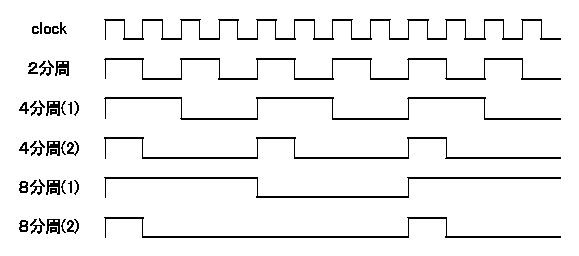
\includegraphics{figure16.eps}
\end{figure}

2分周を超える場合、作られる信号の形は2つのパターンがあります。

一つは、デューティー比( H レベルとL レベルの期間の比)ができるだけ50:50になるよう近づけたパターン。

もう一つは、作り出した周期の中で1クロック分だけH レベルとし、残りはL とするパターン。

通常デバイス内では後者、デバイスの外では前者が使われることが多いです。

4分周の2つめのパターンの例を以下に示します。

プロジェクト名 vhdl08

\begin{Verbatim}[commandchars=\\\{\}]
\PYG{k}{library} \PYG{n+nn}{ieee} \PYG{p}{;}
\PYG{k}{use} \PYG{n+nn}{ieee.std\PYGZus{}logic\PYGZus{}1164.all}\PYG{p}{;}
\PYG{k}{use} \PYG{n+nn}{ieee.std\PYGZus{}logic\PYGZus{}arith.all}\PYG{p}{;}
\PYG{k}{use} \PYG{n+nn}{ieee.std\PYGZus{}logic\PYGZus{}unsigned.all}\PYG{p}{;}

\PYG{k}{entity} \PYG{n+nc}{vhdl08} \PYG{k}{is}
  \PYG{k}{port} \PYG{p}{(}
  \PYG{n}{gclk0} \PYG{o}{:} \PYG{k}{in} \PYG{k+kt}{std\PYGZus{}logic}\PYG{p}{;}
  \PYG{n}{led1} \PYG{o}{:} \PYG{k}{out} \PYG{k+kt}{std\PYGZus{}logic}\PYG{p}{;}
  \PYG{n}{led2} \PYG{o}{:} \PYG{k}{out} \PYG{k+kt}{std\PYGZus{}logic}
  \PYG{p}{)}\PYG{p}{;}
\PYG{k}{end} \PYG{n+nc}{vhdl08}\PYG{p}{;}

\PYG{k}{architecture} \PYG{n+nc}{rtl} \PYG{k}{of} \PYG{n+nc}{vhdl08} \PYG{k}{is}
  \PYG{k}{signal} \PYG{n}{c} \PYG{o}{:} \PYG{k+kt}{std\PYGZus{}logic\PYGZus{}vector} \PYG{p}{(}\PYG{l+m+mi}{1} \PYG{k}{downto} \PYG{l+m+mi}{0}\PYG{p}{)}\PYG{p}{;}
  \PYG{k}{signal} \PYG{n}{r} \PYG{o}{:} \PYG{k+kt}{std\PYGZus{}logic}\PYG{p}{;}
\PYG{k}{begin}
  \PYG{n}{div\PYGZus{}proc} \PYG{o}{:} \PYG{k}{process} \PYG{p}{(}\PYG{n}{gclk0}\PYG{p}{)}
  \PYG{k}{begin}
    \PYG{k}{if} \PYG{p}{(}\PYG{n}{gclk0}\PYG{n+na}{\PYGZsq{}event} \PYG{k}{and} \PYG{n}{gclk0} \PYG{o}{=} \PYG{l+s+sc}{\PYGZsq{}1\PYGZsq{}}\PYG{p}{)} \PYG{k}{then}
      \PYG{n}{c} \PYG{o}{\PYGZlt{}}\PYG{o}{=} \PYG{n}{c} \PYG{o}{+} \PYG{l+m+mi}{1}\PYG{p}{;}
      \PYG{k}{if} \PYG{p}{(}\PYG{n}{c} \PYG{o}{=} \PYG{l+s}{\PYGZdq{}11\PYGZdq{}}\PYG{p}{)} \PYG{k}{then}
        \PYG{n}{r} \PYG{o}{\PYGZlt{}}\PYG{o}{=} \PYG{l+s+sc}{\PYGZsq{}1\PYGZsq{}}\PYG{p}{;}
      \PYG{k}{else}
        \PYG{n}{r} \PYG{o}{\PYGZlt{}}\PYG{o}{=} \PYG{l+s+sc}{\PYGZsq{}0\PYGZsq{}}\PYG{p}{;}
      \PYG{k}{end} \PYG{k}{if}\PYG{p}{;}
    \PYG{k}{end} \PYG{k}{if}\PYG{p}{;}
  \PYG{k}{end} \PYG{k}{process}\PYG{p}{;}

  \PYG{n}{led1} \PYG{o}{\PYGZlt{}}\PYG{o}{=} \PYG{k}{not} \PYG{n}{r}\PYG{p}{;}
  \PYG{n}{led2} \PYG{o}{\PYGZlt{}}\PYG{o}{=} \PYG{l+s+sc}{\PYGZsq{}0\PYGZsq{}}\PYG{p}{;}
\PYG{k}{end} \PYG{n+nc}{rtl}\PYG{p}{;}
\end{Verbatim}

この中で c は10進数で0~3までカウントし、r にはそのうち3のときだけ `1' がセットされます。その反転による LED の点灯がされるため、gclk0 32MHz で4周期のうち1サイクルだけ点灯することになり、結果として単純に点灯している led2 に比べ led1 が暗くなります。
\begin{figure}[htbp]
\centering

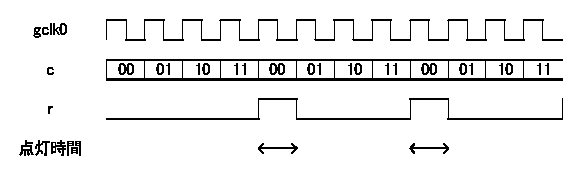
\includegraphics{figure17.eps}
\end{figure}


\subsection{5.9.2 課題}
\label{05_try:id16}
プロジェクト名 vhdl09

約1秒周期でled1 の点灯、消灯を繰り返す回路を作れ
(約0.5 秒点灯、約0.5 秒消灯を繰り返す)

\begin{Verbatim}[commandchars=\\\{\}]
\PYG{k}{library} \PYG{n+nn}{ieee}\PYG{p}{;}
\PYG{k}{use} \PYG{n+nn}{ieee.std\PYGZus{}logic\PYGZus{}1164.all}\PYG{p}{;}
\PYG{k}{use} \PYG{n+nn}{ieee.std\PYGZus{}logic\PYGZus{}arith.all}\PYG{p}{;}
\PYG{k}{use} \PYG{n+nn}{ieee.std\PYGZus{}logic\PYGZus{}unsigned.all}\PYG{p}{;}

\PYG{k}{entity} \PYG{n+nc}{vhdl09} \PYG{k}{is}
  \PYG{k}{port} \PYG{p}{(}
  \PYG{n}{gclk0} \PYG{o}{:} \PYG{k}{in} \PYG{k+kt}{std\PYGZus{}logic}\PYG{p}{;}
  \PYG{n}{led1} \PYG{o}{:} \PYG{k}{out} \PYG{k+kt}{std\PYGZus{}logic}
  \PYG{p}{)}\PYG{p}{;}
\PYG{k}{end} \PYG{n+nc}{vhdl09}\PYG{p}{;}

\PYG{k}{architecture} \PYG{n+nc}{rtl} \PYG{k}{of} \PYG{n+nc}{vhdl09} \PYG{k}{is}
  \PYG{k}{signal} \PYG{n}{c} \PYG{o}{:} \PYG{k+kt}{std\PYGZus{}logic\PYGZus{}vector} \PYG{p}{(}\PYG{l+m+mi}{24} \PYG{k}{downto} \PYG{l+m+mi}{0}\PYG{p}{)}\PYG{p}{;} \PYG{c+c1}{\PYGZhy{}\PYGZhy{} counter}
  \PYG{k}{signal} \PYG{n}{r} \PYG{o}{:} \PYG{k+kt}{std\PYGZus{}logic}\PYG{p}{;} \PYG{c+c1}{\PYGZhy{}\PYGZhy{} invert t when it is H level}
  \PYG{k}{signal} \PYG{n}{t} \PYG{o}{:} \PYG{k+kt}{std\PYGZus{}logic}\PYG{p}{;} \PYG{c+c1}{\PYGZhy{}\PYGZhy{} T flipflop}
\PYG{k}{begin}
  \PYG{n}{cnt\PYGZus{}proc} \PYG{o}{:} \PYG{k}{process} \PYG{p}{(}\PYG{n}{gclk0}\PYG{p}{)}
  \PYG{k}{begin}
    \PYG{k}{if} \PYG{p}{(}\PYG{n}{gclk0}\PYG{n+na}{\PYGZsq{}event} \PYG{k}{and} \PYG{n}{gclk0} \PYG{o}{=} \PYG{l+s+sc}{\PYGZsq{}1\PYGZsq{}}\PYG{p}{)} \PYG{k}{then}
       \PYG{c+c1}{\PYGZhy{}\PYGZhy{} put code below \PYGZhy{}\PYGZhy{}}

       \PYG{c+c1}{\PYGZhy{}\PYGZhy{} put code above \PYGZhy{}\PYGZhy{}}
    \PYG{k}{end} \PYG{k}{if}\PYG{p}{;}
  \PYG{k}{end} \PYG{k}{process}\PYG{p}{;}

  \PYG{n}{t\PYGZus{}proc} \PYG{o}{:} \PYG{k}{process} \PYG{p}{(}\PYG{n}{gclk0}\PYG{p}{)}
  \PYG{k}{begin}
    \PYG{k}{if} \PYG{p}{(}\PYG{n}{gclk0}\PYG{n+na}{\PYGZsq{}event} \PYG{k}{and} \PYG{n}{gclk0} \PYG{o}{=} \PYG{l+s+sc}{\PYGZsq{}1\PYGZsq{}}\PYG{p}{)} \PYG{k}{then}
       \PYG{c+c1}{\PYGZhy{}\PYGZhy{} put code below \PYGZhy{}\PYGZhy{}}

       \PYG{c+c1}{\PYGZhy{}\PYGZhy{} put code above \PYGZhy{}\PYGZhy{}}
    \PYG{k}{end} \PYG{k}{if}\PYG{p}{;}
  \PYG{k}{end} \PYG{k}{process}\PYG{p}{;}

  \PYG{n}{led1} \PYG{o}{\PYGZlt{}}\PYG{o}{=} \PYG{n}{t}\PYG{p}{;}
\PYG{k}{end} \PYG{n+nc}{rtl}\PYG{p}{;}
\end{Verbatim}

分周回路と T フリップフロップ(のような動作)を組み合わせて作成します。基板上、JP5 のジャンパをショートし、gclk0 の周波数を 32MHz に設定します。分周回路は、1クロックだけ H レベルを作るような構成にする必要があります。先ほどの分周回路では ``11'' と比較していたところを、今回は (2\textasciicircum{}25)-1 、つまり''111111111111111111111111''と比較することになります。このときに r を 1 にセットします。

T フリップフロップは単純で、入力信号が 1 であれば反転、0 であればデータを維持します。

r は、32MHz を 33,554,431 回カウントする毎に 1 になるため、そのたびに t が反転されます。それを led1 に出力すれば、目的の回路ができあがります。


\section{5.10 積分回路とチャタリング除去}
\label{05_try:id17}
機械的なスイッチは、切り替えたときに信号の状態が不安定な期間があります。
\begin{figure}[htbp]
\centering

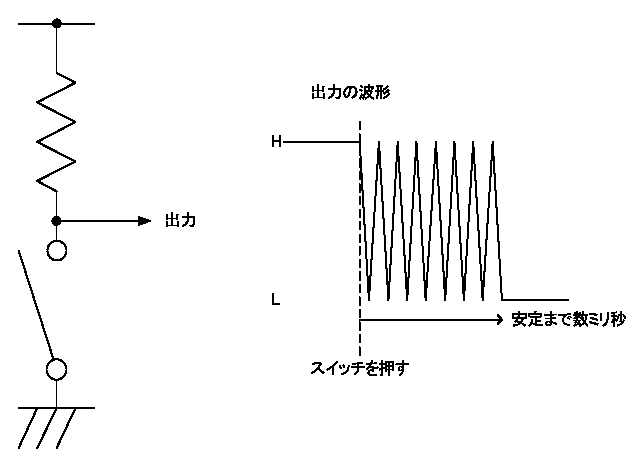
\includegraphics{figure18.eps}
\end{figure}

この不安定な期間は数ms 程度続く場合もあります。人間にとっては感知できないほど短い時間ですが、FPGA は動作が十分速いため、この細かい変化を検出し、反応してしまいます。たとえば課題 vhdl06 ではこれにより不安定な動作となっています。

そのため、それを除去する回路を組み込む必要があります。これには積分回路を応用します。
\begin{figure}[htbp]
\centering

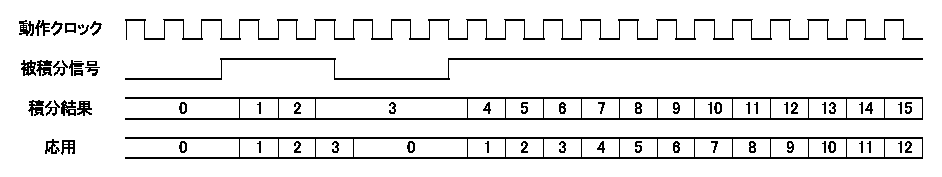
\includegraphics{figure19.eps}
\end{figure}

積分回路は基本的にはカウンタです。入力を単純に加算していきます。これを応用し、H が入力されている間は上限まで加算(上限まで来たら値を維持)、一度でも L が来たら値をクリアします。

この応用した回路に、スイッチからの信号を入力します。スイッチを切り替えない期間では、カウンタの値は0か最大のいずれかで安定します。

スイッチを切り替えた時、入力は H と L が激しく切り替わります。応用した回路では入力の H が一定期間維持されると H を出力するよう動作しますので、この「一定期間」が数ミリ秒となるようなカウンタの最大値を設定すれば良いことになります。
\begin{figure}[htbp]
\centering

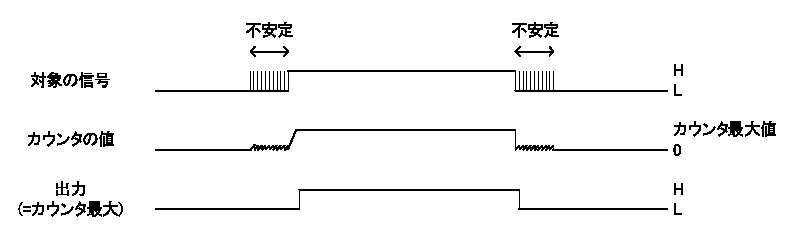
\includegraphics{figure20.eps}
\end{figure}

応用回路はたとえば以下のようなソースになります。clock は積分していくサイクル、sw1 がチャタリングのあるスイッチからの入力、r がチャタリング除去後の出力です。

\begin{Verbatim}[commandchars=\\\{\}]
\PYG{k}{process} \PYG{p}{(}\PYG{n}{clock}\PYG{p}{)}
\PYG{k}{begin}
  \PYG{k}{if} \PYG{p}{(}\PYG{n}{clock}\PYG{n+na}{\PYGZsq{}event} \PYG{k}{and} \PYG{n}{clock} \PYG{o}{=} \PYG{l+s+sc}{\PYGZsq{}1\PYGZsq{}}\PYG{p}{)} \PYG{k}{then}
    \PYG{k}{if} \PYG{p}{(}\PYG{n}{sw1} \PYG{o}{=} \PYG{l+s+sc}{\PYGZsq{}0\PYGZsq{}}\PYG{p}{)} \PYG{k}{then}
      \PYG{n}{c} \PYG{o}{\PYGZlt{}}\PYG{o}{=} \PYG{l+s}{\PYGZdq{}000000000000000\PYGZdq{}}\PYG{p}{;}
    \PYG{k}{elsif} \PYG{p}{(}\PYG{n}{c} \PYG{o}{/}\PYG{o}{=} \PYG{l+s}{\PYGZdq{}111111111111111\PYGZdq{}}\PYG{p}{)} \PYG{k}{and} \PYG{p}{(}\PYG{n}{sw1} \PYG{o}{=} \PYG{l+s+sc}{\PYGZsq{}1\PYGZsq{}}\PYG{p}{)}\PYG{p}{)} \PYG{k}{then}
      \PYG{n}{c} \PYG{o}{\PYGZlt{}}\PYG{o}{=} \PYG{n}{c} \PYG{o}{+} \PYG{l+m+mi}{1}\PYG{p}{;}
    \PYG{k}{end} \PYG{k}{if}\PYG{p}{;}

    \PYG{k}{if} \PYG{p}{(}\PYG{n}{c} \PYG{o}{=} \PYG{l+s}{\PYGZdq{}111111111111111\PYGZdq{}}\PYG{p}{)} \PYG{k}{then}
      \PYG{n}{r} \PYG{o}{\PYGZlt{}}\PYG{o}{=} \PYG{l+s+sc}{\PYGZsq{}1\PYGZsq{}}\PYG{p}{;}
    \PYG{k}{else}
      \PYG{n}{r} \PYG{o}{\PYGZlt{}}\PYG{o}{=} \PYG{l+s+sc}{\PYGZsq{}0\PYGZsq{}}\PYG{p}{;}
    \PYG{k}{end} \PYG{k}{if}\PYG{p}{;}
  \PYG{k}{end} \PYG{k}{if}\PYG{p}{;}
\PYG{k}{end} \PYG{k}{process}\PYG{p}{;}
\end{Verbatim}

最初のif 文では、カウンタによる積分回路を構成しています。

スイッチが離されたら(sw1 = `0')カウンタの値は即0とします。

スイッチが押された場合(sw1 = `1')、カウンタがいっぱいでなければ(c /= ``111111111111111''、''/=''は''一致していない'' の意味)カウントします(c \textless{}= c + 1)。

このカウンタは、スイッチが押されれば、カウンタのビットがすべて1になるまでカウントを続け、離されるとすぐにすべて0に戻します。

スイッチからの信号が不安定な状態では、少しでも0がくればカウンタも0に戻されますが、十分安定すれば最後までカウントします。

32MHz であれば1周期は約 31nsなので、15bit で 32000 回カウントすれば約1msになります。スイッチが約1ms安定すれば、最後までカウントされることになります。

次の if 文では、前のカウンタが最後までカウントされたら1、それ以外は0を出力します。スイッチ入力が安定したことを判定することができます。

このままでは1msしか対応できないため、チャタリングが除去し切れていないように見える場合はカウンタのビットを追加する必要があります。


\section{5.11 微分回路}
\label{05_try:id18}
人間や機械からの信号= 遅い信号と高速な内部の回路とのインタフェースをしやすくする回路です。

たとえばスイッチを動かす度に LED の点灯、消灯を切り替えたいとします。タイミングチャートは以下のようなものです。
\begin{figure}[htbp]
\centering

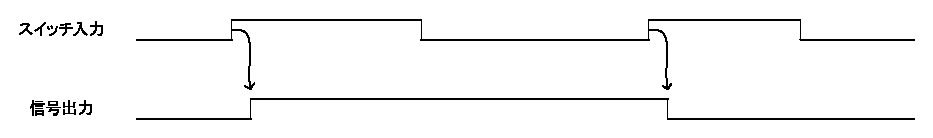
\includegraphics{figure21.eps}
\end{figure}

スイッチ入力をクロックとしてT フリップフロップに入力できれば実現できますが、同期動作ではないためトラブルの原因になりやすく、採用できません。

出力の信号を生成しているフリップフロップのクロックが十分遅ければやはり T フリップフロップで対応できそうですが、今回のボードに限らず通常は MHz 級の動作周波数ですのでそのような動作はできません。
\begin{figure}[htbp]
\centering

\includegraphics{figure22.eps}
\end{figure}

スイッチ入力の変化点を検出する回路ができれば、T フリップフロップでも望みの動作が可能になります。
\begin{figure}[htbp]
\centering

\includegraphics{figure23.eps}
\end{figure}

変化点を検出するため、微分回路と呼ばれる回路を使用します。
\begin{figure}[htbp]
\centering

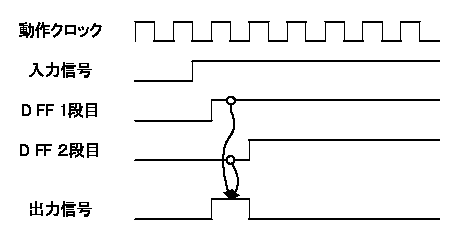
\includegraphics{figure24.eps}
\end{figure}

原理は簡単で、フリップフロップ2段を通して1クロックずつ遅延した信号の間の特定の差だけを抽出します。

実際の回路は以下のようになります。
\begin{figure}[htbp]
\centering

\includegraphics{figure25.eps}
\end{figure}


\subsection{5.11.1 演習}
\label{05_try:id19}
プロジェクト名vhdl10

スイッチを押す度にLED の点灯、消灯を切り替える回路を作る。

\begin{Verbatim}[commandchars=\\\{\}]
\PYG{k}{library} \PYG{n+nn}{ieee}\PYG{p}{;}
\PYG{k}{use} \PYG{n+nn}{ieee.std\PYGZus{}logic\PYGZus{}1164.all}\PYG{p}{;}
\PYG{k}{use} \PYG{n+nn}{ieee.std\PYGZus{}logic\PYGZus{}arith.all}\PYG{p}{;}
\PYG{k}{use} \PYG{n+nn}{ieee.std\PYGZus{}logic\PYGZus{}unsigned.all}\PYG{p}{;}

\PYG{k}{entity} \PYG{n+nc}{vhdl10} \PYG{k}{is}
  \PYG{k}{port} \PYG{p}{(}
    \PYG{n}{gclk0} \PYG{o}{:} \PYG{k}{in} \PYG{k+kt}{std\PYGZus{}logic}\PYG{p}{;}
    \PYG{n}{sw1} \PYG{o}{:} \PYG{k}{in} \PYG{k+kt}{std\PYGZus{}logic}\PYG{p}{;}
    \PYG{n}{led1} \PYG{o}{:} \PYG{k}{out} \PYG{k+kt}{std\PYGZus{}logic}
  \PYG{p}{)}\PYG{p}{;}
\PYG{k}{end} \PYG{n+nc}{vhdl10}\PYG{p}{;}

\PYG{k}{architecture} \PYG{n}{rtl} \PYG{n}{o} \PYG{n}{f} \PYG{n}{vhdl10} \PYG{k}{is}
  \PYG{k}{signal} \PYG{n}{c} \PYG{o}{:} \PYG{k+kt}{std\PYGZus{}logic\PYGZus{}vector} \PYG{p}{(}\PYG{l+m+mi}{14} \PYG{k}{downto} \PYG{l+m+mi}{0}\PYG{p}{)}\PYG{p}{;}
  \PYG{k}{signal} \PYG{n}{r} \PYG{o}{:} \PYG{k+kt}{std\PYGZus{}logic}\PYG{p}{;}
  \PYG{k}{signal} \PYG{n}{d1} \PYG{o}{:} \PYG{k+kt}{std\PYGZus{}logic}\PYG{p}{;}
  \PYG{k}{signal} \PYG{n}{d2} \PYG{o}{:} \PYG{k+kt}{std\PYGZus{}logic}\PYG{p}{;}
  \PYG{k}{signal} \PYG{n}{s} \PYG{o}{:} \PYG{k+kt}{std\PYGZus{}logic}\PYG{p}{;}
  \PYG{k}{signal} \PYG{n}{t} \PYG{o}{:} \PYG{k+kt}{std\PYGZus{}logic}\PYG{p}{;}
\PYG{k}{begin}
  \PYG{c+c1}{\PYGZhy{}\PYGZhy{} chattering cancel}
  \PYG{n}{sum\PYGZus{}proc} \PYG{o}{:} \PYG{k}{process} \PYG{p}{(}\PYG{n}{gclk0}\PYG{p}{)}
  \PYG{k}{begin}
    \PYG{k}{if} \PYG{p}{(}\PYG{n}{gclk0}\PYG{n+na}{\PYGZsq{}event} \PYG{k}{and} \PYG{n}{gclk0} \PYG{o}{=} \PYG{l+s+sc}{\PYGZsq{}1\PYGZsq{}}\PYG{p}{)} \PYG{k}{then}
      \PYG{k}{if} \PYG{p}{(}\PYG{n}{sw1} \PYG{o}{=} \PYG{l+s+sc}{\PYGZsq{}0\PYGZsq{}}\PYG{p}{)} \PYG{k}{then}
        \PYG{n}{c} \PYG{o}{\PYGZlt{}}\PYG{o}{=} \PYG{l+s}{\PYGZdq{}000000000000000\PYGZdq{}}\PYG{p}{;}
      \PYG{k}{elsif} \PYG{p}{(}\PYG{p}{(}\PYG{n}{c} \PYG{o}{/}\PYG{o}{=} \PYG{l+s}{\PYGZdq{}111111111111111\PYGZdq{}}\PYG{p}{)} \PYG{k}{and} \PYG{p}{(}\PYG{n}{sw1} \PYG{o}{=} \PYG{l+s+sc}{\PYGZsq{}1\PYGZsq{}}\PYG{p}{)}\PYG{p}{)} \PYG{k}{then}
        \PYG{n}{c} \PYG{o}{\PYGZlt{}}\PYG{o}{=} \PYG{n}{c} \PYG{o}{+} \PYG{l+m+mi}{1}\PYG{p}{;}
      \PYG{k}{end} \PYG{k}{if}\PYG{p}{;}

      \PYG{k}{if} \PYG{p}{(}\PYG{n}{c} \PYG{o}{=} \PYG{l+s}{\PYGZdq{}111111111111111\PYGZdq{}}\PYG{p}{)} \PYG{k}{then}
        \PYG{n}{r} \PYG{o}{\PYGZlt{}}\PYG{o}{=} \PYG{l+s+sc}{\PYGZsq{}1\PYGZsq{}}\PYG{p}{;}
      \PYG{k}{else}
        \PYG{n}{r} \PYG{o}{\PYGZlt{}}\PYG{o}{=} \PYG{l+s+sc}{\PYGZsq{}0\PYGZsq{}}\PYG{p}{;}
      \PYG{k}{end} \PYG{k}{if}\PYG{p}{;}
    \PYG{k}{end} \PYG{k}{if}\PYG{p}{;}
  \PYG{k}{end} \PYG{k}{process}\PYG{p}{;}

  \PYG{c+c1}{\PYGZhy{}\PYGZhy{} difference}
  \PYG{n}{diff\PYGZus{}proc} \PYG{o}{:} \PYG{k}{process} \PYG{p}{(}\PYG{n}{gclk0}\PYG{p}{)}
  \PYG{k}{begin}
    \PYG{k}{if} \PYG{p}{(}\PYG{n}{gclk0}\PYG{n+na}{\PYGZsq{}event} \PYG{k}{and} \PYG{n}{gclk0} \PYG{o}{=} \PYG{l+s+sc}{\PYGZsq{}1\PYGZsq{}}\PYG{p}{)} \PYG{k}{then}
      \PYG{n}{d1} \PYG{o}{\PYGZlt{}}\PYG{o}{=} \PYG{n}{r}\PYG{p}{;}
      \PYG{n}{d2} \PYG{o}{\PYGZlt{}}\PYG{o}{=} \PYG{n}{d1}\PYG{p}{;}
    \PYG{k}{end} \PYG{k}{if}\PYG{p}{;}
  \PYG{k}{end} \PYG{k}{process}\PYG{p}{;}
  \PYG{n}{s} \PYG{o}{\PYGZlt{}}\PYG{o}{=} \PYG{n}{d1} \PYG{k}{and} \PYG{p}{(}\PYG{k}{not} \PYG{n}{d2}\PYG{p}{)}\PYG{p}{;}

  \PYG{c+c1}{\PYGZhy{}\PYGZhy{} T flipflop}
  \PYG{n}{t\PYGZus{}proc} \PYG{o}{:} \PYG{k}{process} \PYG{p}{(}\PYG{n}{gclk0}\PYG{p}{)}
  \PYG{k}{begin}
    \PYG{k}{if} \PYG{p}{(}\PYG{n}{gclk0}\PYG{n+na}{\PYGZsq{}event} \PYG{k}{and} \PYG{n}{gclk0} \PYG{o}{=} \PYG{l+s+sc}{\PYGZsq{}1\PYGZsq{}}\PYG{p}{)} \PYG{k}{then}
      \PYG{k}{if} \PYG{p}{(}\PYG{n}{s} \PYG{o}{=} \PYG{l+s+sc}{\PYGZsq{}1\PYGZsq{}}\PYG{p}{)} \PYG{k}{then}
        \PYG{n}{t} \PYG{o}{\PYGZlt{}}\PYG{o}{=} \PYG{k}{not} \PYG{n}{t}\PYG{p}{;}
      \PYG{k}{end} \PYG{k}{if}\PYG{p}{;}
    \PYG{k}{end} \PYG{k}{if}\PYG{p}{;}
  \PYG{k}{end} \PYG{k}{process}\PYG{p}{;}

  \PYG{n}{led1} \PYG{o}{\PYGZlt{}}\PYG{o}{=} \PYG{n}{t}\PYG{p}{;}
\PYG{k}{end} \PYG{n+nc}{rtl}\PYG{p}{;}
\end{Verbatim}

diff proc とその直後の s への代入が微分回路になります。


\section{5.12 10進カウンタ}
\label{05_try:id20}

\subsection{5.12.1 課題}
\label{05_try:id21}
プロジェクト名 vhdl11

0~9まで、1秒間に1ずつカウントする、10進カウンタを作れ。カウント値は9の次は0に戻る。
signal r は1秒に1回、1サイクルだけH レベルになる信号となる。
led1 が点滅する場合は誤りがある。

\begin{Verbatim}[commandchars=\\\{\}]
\PYG{k}{library} \PYG{n+nn}{ieee} \PYG{p}{;}
\PYG{k}{use} \PYG{n+nn}{ieee.std\PYGZus{}logic\PYGZus{}1164.all}\PYG{p}{;}
\PYG{k}{use} \PYG{n+nn}{ieee.std\PYGZus{}logic\PYGZus{}arith.all}\PYG{p}{;}
\PYG{k}{use} \PYG{n+nn}{ieee.std\PYGZus{}logic\PYGZus{}unsigned.all}\PYG{p}{;}

\PYG{k}{entity} \PYG{n+nc}{vhdl11} \PYG{k}{is}
  \PYG{k}{port} \PYG{p}{(}
    \PYG{n}{gclk0} \PYG{o}{:} \PYG{k}{in} \PYG{k+kt}{std\PYGZus{}logic}\PYG{p}{;}
    \PYG{n}{led1} \PYG{o}{:} \PYG{k}{out} \PYG{k+kt}{std\PYGZus{}logic}\PYG{p}{;}
    \PYG{n}{sled1a} \PYG{o}{:} \PYG{k}{out} \PYG{k+kt}{std\PYGZus{}logic}\PYG{p}{;}
    \PYG{n}{sled1b} \PYG{o}{:} \PYG{k}{out} \PYG{k+kt}{std\PYGZus{}logic}\PYG{p}{;}
    \PYG{n}{sled1c} \PYG{o}{:} \PYG{k}{out} \PYG{k+kt}{std\PYGZus{}logic}\PYG{p}{;}
    \PYG{n}{sled1d} \PYG{o}{:} \PYG{k}{out} \PYG{k+kt}{std\PYGZus{}logic}\PYG{p}{;}
    \PYG{n}{sled1e} \PYG{o}{:} \PYG{k}{out} \PYG{k+kt}{std\PYGZus{}logic}\PYG{p}{;}
    \PYG{n}{sled1f} \PYG{o}{:} \PYG{k}{out} \PYG{k+kt}{std\PYGZus{}logic}\PYG{p}{;}
    \PYG{n}{sled1g} \PYG{o}{:} \PYG{k}{out} \PYG{k+kt}{std\PYGZus{}logic}
  \PYG{p}{)}\PYG{p}{;}
\PYG{k}{end} \PYG{n+nc}{vhdl11}\PYG{p}{;}

\PYG{k}{architecture} \PYG{n+nc}{rtl} \PYG{k}{of} \PYG{n+nc}{vhdl11} \PYG{k}{is}
  \PYG{k}{signal} \PYG{n}{d} \PYG{o}{:} \PYG{k+kt}{std\PYGZus{}logic\PYGZus{}vector} \PYG{p}{(}\PYG{l+m+mi}{24} \PYG{k}{downto} \PYG{l+m+mi}{0}\PYG{p}{)}\PYG{p}{;}
  \PYG{k}{signal} \PYG{n}{r} \PYG{o}{:} \PYG{k+kt}{std\PYGZus{}logic}\PYG{p}{;}
  \PYG{k}{signal} \PYG{n}{c} \PYG{o}{:} \PYG{k+kt}{std\PYGZus{}logic\PYGZus{}vector} \PYG{p}{(}\PYG{l+m+mi}{3} \PYG{k}{downto} \PYG{l+m+mi}{0}\PYG{p}{)}\PYG{p}{;}
  \PYG{k}{signal} \PYG{n}{s} \PYG{n}{l} \PYG{n}{e} \PYG{n}{d} \PYG{o}{:} \PYG{k+kt}{std\PYGZus{}logic\PYGZus{}vector} \PYG{p}{(}\PYG{l+m+mi}{6} \PYG{k}{downto} \PYG{l+m+mi}{0}\PYG{p}{)}\PYG{p}{;}
  \PYG{k}{signal} \PYG{n}{ck} \PYG{o}{:} \PYG{k+kt}{std\PYGZus{}logic}\PYG{p}{;}
\PYG{k}{begin}
  \PYG{n}{div\PYGZus{}proc} \PYG{o}{:} \PYG{k}{process} \PYG{p}{(}\PYG{n}{gclk0}\PYG{p}{)}
  \PYG{k}{begin}
    \PYG{k}{if} \PYG{p}{(}\PYG{n}{gclk0}\PYG{n+na}{\PYGZsq{}event} \PYG{k}{and} \PYG{n}{gclk0} \PYG{o}{=} \PYG{l+s+sc}{\PYGZsq{}1\PYGZsq{}}\PYG{p}{)} \PYG{k}{then}
      \PYG{n}{d} \PYG{o}{\PYGZlt{}}\PYG{o}{=} \PYG{n}{d} \PYG{o}{+} \PYG{l+m+mi}{1}\PYG{p}{;}
      \PYG{k}{if} \PYG{p}{(}\PYG{n}{d} \PYG{o}{=} \PYG{l+s}{\PYGZdq{}1111010000100011111111111\PYGZdq{}}\PYG{p}{)} \PYG{k}{then}
        \PYG{n}{r} \PYG{o}{\PYGZlt{}}\PYG{o}{=} \PYG{l+s+sc}{\PYGZsq{}1\PYGZsq{}}\PYG{p}{;}
        \PYG{n}{d} \PYG{o}{\PYGZlt{}}\PYG{o}{=} \PYG{l+s}{\PYGZdq{}0000000000000000000000000\PYGZdq{}}\PYG{p}{;}
      \PYG{k}{else}
        \PYG{n}{r} \PYG{o}{\PYGZlt{}}\PYG{o}{=} \PYG{l+s+sc}{\PYGZsq{}0\PYGZsq{}}\PYG{p}{;}
      \PYG{k}{end} \PYG{k}{if}\PYG{p}{;}
    \PYG{k}{end} \PYG{k}{if}\PYG{p}{;}
  \PYG{k}{end} \PYG{k}{process}\PYG{p}{;}

  \PYG{n}{cnt\PYGZus{}proc} \PYG{o}{:} \PYG{k}{process} \PYG{p}{(}\PYG{n}{gclk0}\PYG{p}{)}
  \PYG{k}{begin}
    \PYG{k}{if} \PYG{p}{(}\PYG{n}{gclk0}\PYG{n+na}{\PYGZsq{}event} \PYG{k}{and} \PYG{n}{gclk0} \PYG{o}{=} \PYG{l+s+sc}{\PYGZsq{}1\PYGZsq{}}\PYG{p}{)} \PYG{k}{then}
       \PYG{c+c1}{\PYGZhy{}\PYGZhy{} put code below \PYGZhy{}\PYGZhy{}}

       \PYG{c+c1}{\PYGZhy{}\PYGZhy{} put code above \PYGZhy{}\PYGZhy{}}
    \PYG{k}{end} \PYG{k}{if}\PYG{p}{;}
  \PYG{k}{end} \PYG{k}{process}\PYG{p}{;}

  \PYG{n}{chk\PYGZus{}proc} \PYG{o}{:} \PYG{k}{process} \PYG{p}{(}\PYG{n}{gclk0}\PYG{p}{)}
  \PYG{k}{begin}
    \PYG{k}{if} \PYG{p}{(}\PYG{n}{gclk0}\PYG{n+na}{\PYGZsq{}event} \PYG{k}{and} \PYG{n}{gclk0} \PYG{o}{=} \PYG{l+s+sc}{\PYGZsq{}1\PYGZsq{}}\PYG{p}{)} \PYG{k}{then}
      \PYG{k}{if} \PYG{p}{(}\PYG{n}{c} \PYG{o}{=} \PYG{l+s}{\PYGZdq{}1010\PYGZdq{}}\PYG{p}{)} \PYG{k}{then}
        \PYG{n}{ck} \PYG{o}{\PYGZlt{}}\PYG{o}{=} \PYG{k}{not} \PYG{n}{ck}\PYG{p}{;}
      \PYG{k}{end} \PYG{k}{if}\PYG{p}{;}
    \PYG{k}{end} \PYG{k}{if}\PYG{p}{;}
  \PYG{k}{end} \PYG{k}{process}\PYG{p}{;}

  \PYG{n}{sled} \PYG{o}{\PYGZlt{}}\PYG{o}{=} \PYG{l+s}{\PYGZdq{}0010000\PYGZdq{} when (c = \PYGZdq{}1001\PYGZdq{}}\PYG{p}{)}
     \PYG{k}{else} \PYG{l+s}{\PYGZdq{}0000000\PYGZdq{} when (c = \PYGZdq{}1000\PYGZdq{}}\PYG{p}{)}
     \PYG{k}{else} \PYG{l+s}{\PYGZdq{}1111000\PYGZdq{} when (c = \PYGZdq{}0111\PYGZdq{}}\PYG{p}{)}
     \PYG{k}{else} \PYG{l+s}{\PYGZdq{}0000010\PYGZdq{} when (c = \PYGZdq{}0110\PYGZdq{}}\PYG{p}{)}
     \PYG{k}{else} \PYG{l+s}{\PYGZdq{}0010010\PYGZdq{} when (c = \PYGZdq{}0101\PYGZdq{}}\PYG{p}{)}
     \PYG{k}{else} \PYG{l+s}{\PYGZdq{}0011001\PYGZdq{} when (c = \PYGZdq{}0100\PYGZdq{}}\PYG{p}{)}
     \PYG{k}{else} \PYG{l+s}{\PYGZdq{}0110000\PYGZdq{} when (c = \PYGZdq{}0011\PYGZdq{}}\PYG{p}{)}
     \PYG{k}{else} \PYG{l+s}{\PYGZdq{}0100100\PYGZdq{} when (c = \PYGZdq{}0010\PYGZdq{}}\PYG{p}{)}
     \PYG{k}{else} \PYG{l+s}{\PYGZdq{}1111001\PYGZdq{} when (c = \PYGZdq{}0001\PYGZdq{}}\PYG{p}{)}
     \PYG{k}{else} \PYG{l+s}{\PYGZdq{}1000000\PYGZdq{} when (c = \PYGZdq{}0000\PYGZdq{}}\PYG{p}{)}
     \PYG{k}{else} \PYG{l+s}{\PYGZdq{}0000110\PYGZdq{}}\PYG{p}{;}
  \PYG{n}{sled1a} \PYG{o}{\PYGZlt{}}\PYG{o}{=} \PYG{n}{sled} \PYG{p}{(}\PYG{l+m+mi}{0}\PYG{p}{)}\PYG{p}{;}
  \PYG{n}{sled1b} \PYG{o}{\PYGZlt{}}\PYG{o}{=} \PYG{n}{sled} \PYG{p}{(}\PYG{l+m+mi}{1}\PYG{p}{)}\PYG{p}{;}
  \PYG{n}{sled1c} \PYG{o}{\PYGZlt{}}\PYG{o}{=} \PYG{n}{sled} \PYG{p}{(}\PYG{l+m+mi}{2}\PYG{p}{)}\PYG{p}{;}
  \PYG{n}{sled1d} \PYG{o}{\PYGZlt{}}\PYG{o}{=} \PYG{n}{sled} \PYG{p}{(}\PYG{l+m+mi}{3}\PYG{p}{)}\PYG{p}{;}
  \PYG{n}{sled1e} \PYG{o}{\PYGZlt{}}\PYG{o}{=} \PYG{n}{sled} \PYG{p}{(}\PYG{l+m+mi}{4}\PYG{p}{)}\PYG{p}{;}
  \PYG{n}{sled1f} \PYG{o}{\PYGZlt{}}\PYG{o}{=} \PYG{n}{sled} \PYG{p}{(}\PYG{l+m+mi}{5}\PYG{p}{)}\PYG{p}{;}
  \PYG{n}{sled1g} \PYG{o}{\PYGZlt{}}\PYG{o}{=} \PYG{n}{sled} \PYG{p}{(}\PYG{l+m+mi}{6}\PYG{p}{)}\PYG{p}{;}

  \PYG{n}{led1} \PYG{o}{\PYGZlt{}}\PYG{o}{=} \PYG{n}{ck}\PYG{p}{;}
\PYG{k}{end} \PYG{n+nc}{rtl}\PYG{p}{;}
\end{Verbatim}

7セグメント LED の点灯パターンはコードの通りになる、LED の配置は図のようになっています。port に L を出力すると、電位差で電流が流れLED が点灯します。
\begin{figure}[htbp]
\centering

\includegraphics{figure26.eps}
\end{figure}


\section{5.13 階層設計}
\label{05_try:id22}
規模が大きくなってくると、すべてのコードを一つのarchitecture に書ききることが問題になります。そのためコードを機能ブロック毎に分割し呼び出すことができるようになっています。
例を以下に示します。

\begin{Verbatim}[commandchars=\\\{\}]
library ieee;
use ieee.std\PYGZus{}logic\PYGZus{}1164.all;
use ieee.std\PYGZus{}logic\PYGZus{}arith.all;
use ieee.std\PYGZus{}logic\PYGZus{}unsigned.all;

entity Y\PYGZus{}child is
  port (
  ~ PORT\PYGZus{}DEFINITION(CHILD) ~
  );
end Y child ;

architecture A\PYGZus{}Y\PYGZus{}child of Y\PYGZus{}child is
  ~ SIGNAL\PYGZus{}DEFINITION(CHILD) ~
begin
  ~ EXPRESSIONS(CHILD) ~
end A Y chi ld ;


library ieee ;
use ieee.std\PYGZus{}logic\PYGZus{}1164.all;
use ieee.std\PYGZus{}logic\PYGZus{}arith.all;
use ieee.std\PYGZus{}logic\PYGZus{}unsigned.all;

entity X\PYGZus{}parent is
  port (
    ~ PORT\PYGZus{}DEFINITION(PARENT) ~
  );
end X\PYGZus{}parent;

architecture A\PYGZus{}X\PYGZus{}parent of X\PYGZus{}parent is

  component Y\PYGZus{}child
    port (
      ~ PORT\PYGZus{}DEFINITION(CHILD) ~
    );
  end component;

  ~ SIGNAL\PYGZus{}DEFINITION(PARENT) ~

begin

  i\PYGZus{}Y\PYGZus{}child : Y\PYGZus{}child
    port map (
      ~ PORT\PYGZus{}CONNECTION(CHILD PARENT) ~
    );

  ~ OTHER\PYGZus{}EXPRESSIONS(PARENT) ~

end A\PYGZus{}X\PYGZus{}parent;
\end{Verbatim}

処理を抜き出した、他から呼び出される側の entity は、通常通り作成します。

処理を呼び出す場合は2段階の手続きがあります。

まず architecture から begin までの間で、component 宣言を行います。ここで、呼び出す entity はすべて宣言します。

次に begin の後で、実際に呼び出します。複数個呼び出すこともできますが、その場合は entity 名の前のコロンの前、インスタンス名(ここでは i\_Y\_child )はそれぞれ固有のものにします。

10進数カウンタに階層化を適用します。

\begin{notice}{note}{注釈:}
counter10.vhd とledconv.vhd は、vhdl11b プロジェクトを作成した後、それぞれ vhdl11b.vhd と同様にfile \(\rightarrow\) new \(\rightarrow\) VHDL file で作成します。
\end{notice}

counter10.vhd

\begin{Verbatim}[commandchars=\\\{\}]
\PYG{k}{library} \PYG{n+nn}{ieee}\PYG{p}{;}
\PYG{k}{use} \PYG{n+nn}{ieee.std\PYGZus{}logic\PYGZus{}1164.all}\PYG{p}{;}
\PYG{k}{use} \PYG{n+nn}{ieee.std\PYGZus{}logic\PYGZus{}arith.all}\PYG{p}{;}
\PYG{k}{use} \PYG{n+nn}{ieee.std\PYGZus{}logic\PYGZus{}unsigned.all}\PYG{p}{;}

\PYG{k}{entity} \PYG{n+nc}{counter10} \PYG{k}{is}
  \PYG{k}{port} \PYG{p}{(}
    \PYG{n}{gclk0} \PYG{o}{:} \PYG{k}{in} \PYG{k+kt}{std\PYGZus{}logic}\PYG{p}{;}
    \PYG{n}{sw1} \PYG{o}{:} \PYG{k}{in} \PYG{k+kt}{std\PYGZus{}logic}\PYG{p}{;}

    \PYG{n}{e\PYGZus{}in} \PYG{o}{:} \PYG{k}{in} \PYG{k+kt}{std\PYGZus{}logic}\PYG{p}{;}
    \PYG{n}{c\PYGZus{}in} \PYG{o}{:} \PYG{k}{in} \PYG{k+kt}{std\PYGZus{}logic}\PYG{p}{;}

    \PYG{n}{c\PYGZus{}out} \PYG{o}{:} \PYG{k}{out} \PYG{k+kt}{std\PYGZus{}logic}\PYG{p}{;}

    \PYG{n}{cnt} \PYG{o}{:} \PYG{k}{out} \PYG{k+kt}{std\PYGZus{}logic\PYGZus{}vector} \PYG{p}{(}\PYG{l+m+mi}{3} \PYG{k}{downto} \PYG{l+m+mi}{0}\PYG{p}{)}
\PYG{p}{)} \PYG{p}{;}
\PYG{k}{end} \PYG{n+nc}{counte} \PYG{n+nc}{r10} \PYG{p}{;}

\PYG{k}{architecture} \PYG{n+nc}{rtl} \PYG{k}{of} \PYG{n+nc}{counter10} \PYG{k}{is}
  \PYG{k}{signal} \PYG{n}{c} \PYG{o}{:} \PYG{k+kt}{std\PYGZus{}logic\PYGZus{}vector} \PYG{p}{(}\PYG{l+m+mi}{3} \PYG{k}{downto} \PYG{l+m+mi}{0}\PYG{p}{)}\PYG{p}{;}
\PYG{k}{begin}
  \PYG{n}{cnt\PYGZus{}proc} \PYG{o}{:} \PYG{k}{process} \PYG{p}{(}\PYG{n}{sw1}\PYG{p}{,} \PYG{n}{gclk0}\PYG{p}{)}
  \PYG{k}{begin}
    \PYG{k}{if} \PYG{p}{(}\PYG{n}{sw1} \PYG{o}{=} \PYG{l+s+sc}{\PYGZsq{}1\PYGZsq{}}\PYG{p}{)} \PYG{k}{then}
      \PYG{n}{c} \PYG{o}{\PYGZlt{}}\PYG{o}{=} \PYG{l+s}{\PYGZdq{}0000\PYGZdq{}}\PYG{p}{;}
    \PYG{k}{elsif} \PYG{p}{(}\PYG{n}{gclk0}\PYG{n+na}{\PYGZsq{}event} \PYG{k}{and} \PYG{n}{gclk0} \PYG{o}{=} \PYG{l+s+sc}{\PYGZsq{}1\PYGZsq{}}\PYG{p}{)} \PYG{k}{then}
      \PYG{k}{if} \PYG{p}{(}\PYG{p}{(}\PYG{n}{e\PYGZus{}in} \PYG{o}{=} \PYG{l+s+sc}{\PYGZsq{}1\PYGZsq{}}\PYG{p}{)} \PYG{k}{and} \PYG{p}{(}\PYG{n}{c\PYGZus{}in} \PYG{o}{=} \PYG{l+s+sc}{\PYGZsq{}1\PYGZsq{}}\PYG{p}{)}\PYG{p}{)} \PYG{k}{then}
        \PYG{c+c1}{\PYGZhy{}\PYGZhy{} put code below \PYGZhy{}\PYGZhy{}}

        \PYG{c+c1}{\PYGZhy{}\PYGZhy{} put code above \PYGZhy{}\PYGZhy{}}
      \PYG{k}{end} \PYG{k}{if}\PYG{p}{;}
    \PYG{k}{end} \PYG{k}{if}\PYG{p}{;}
  \PYG{k}{end} \PYG{k}{process}\PYG{p}{;}

  \PYG{n}{c\PYGZus{}out} \PYG{o}{\PYGZlt{}}\PYG{o}{=} \PYG{l+s+sc}{\PYGZsq{}1\PYGZsq{}} \PYG{k}{when} \PYG{p}{(}\PYG{n}{c} \PYG{o}{=} \PYG{l+s}{\PYGZdq{}1001\PYGZdq{}}\PYG{p}{)}
      \PYG{k}{else} \PYG{l+s+sc}{\PYGZsq{}0\PYGZsq{}}\PYG{p}{;}
  \PYG{n}{cnt} \PYG{o}{\PYGZlt{}}\PYG{o}{=} \PYG{n}{c}\PYG{p}{;}
\PYG{k}{end} \PYG{n+nc}{rtl}\PYG{p}{;}
\end{Verbatim}

c\_in は下の桁からの桁上げのリクエストを受け付けるポート、c\_out は上の桁への桁上げのリクエストを出力するポート。

e\_in はH レベルが入るとカウントを行うポート

ledconv.vhd

\begin{Verbatim}[commandchars=\\\{\}]
\PYG{k}{library} \PYG{n+nn}{ieee}\PYG{p}{;}
\PYG{k}{use} \PYG{n+nn}{ieee.std\PYGZus{}logic\PYGZus{}1164.all}\PYG{p}{;}
\PYG{k}{use} \PYG{n+nn}{ieee.std\PYGZus{}logic\PYGZus{}arith.all}\PYG{p}{;}
\PYG{k}{use} \PYG{n+nn}{ieee.std\PYGZus{}logic\PYGZus{}unsigned.all}\PYG{p}{;}

\PYG{k}{entity} \PYG{n+nc}{ledconv} \PYG{k}{is}
  \PYG{k}{port} \PYG{p}{(}
    \PYG{n}{cnt} \PYG{o}{:} \PYG{k}{in} \PYG{k+kt}{std\PYGZus{}logic\PYGZus{}vector} \PYG{p}{(}\PYG{l+m+mi}{3} \PYG{k}{downto} \PYG{l+m+mi}{0}\PYG{p}{)}\PYG{p}{;}
    \PYG{n}{sledxa} \PYG{o}{:} \PYG{k}{out} \PYG{k+kt}{std\PYGZus{}logic}\PYG{p}{;}
    \PYG{n}{sledxb} \PYG{o}{:} \PYG{k}{out} \PYG{k+kt}{std\PYGZus{}logic}\PYG{p}{;}
    \PYG{n}{sledxc} \PYG{o}{:} \PYG{k}{out} \PYG{k+kt}{std\PYGZus{}logic}\PYG{p}{;}
    \PYG{n}{sledxd} \PYG{o}{:} \PYG{k}{out} \PYG{k+kt}{std\PYGZus{}logic}\PYG{p}{;}
    \PYG{n}{sledxe} \PYG{o}{:} \PYG{k}{out} \PYG{k+kt}{std\PYGZus{}logic}\PYG{p}{;}
    \PYG{n}{sledxf} \PYG{o}{:} \PYG{k}{out} \PYG{k+kt}{std\PYGZus{}logic}\PYG{p}{;}
    \PYG{n}{sledxg} \PYG{o}{:} \PYG{k}{out} \PYG{k+kt}{std\PYGZus{}logic}
  \PYG{p}{)}\PYG{p}{;}
\PYG{k}{end} \PYG{n+nc}{ledconv}\PYG{p}{;}

\PYG{k}{architecture} \PYG{n+nc}{rtl} \PYG{k}{of} \PYG{n+nc}{ledconv} \PYG{k}{is}
  \PYG{k}{signal} \PYG{n}{sled} \PYG{o}{:} \PYG{k+kt}{std\PYGZus{}logic\PYGZus{}vector} \PYG{p}{(}\PYG{l+m+mi}{6} \PYG{k}{downto} \PYG{l+m+mi}{0}\PYG{p}{)}\PYG{p}{;}
\PYG{k}{begin}
  \PYG{n}{sled} \PYG{o}{\PYGZlt{}}\PYG{o}{=} \PYG{l+s}{\PYGZdq{}0010000\PYGZdq{} when (cnt = \PYGZdq{}1001\PYGZdq{}}\PYG{p}{)}
     \PYG{k}{else} \PYG{l+s}{\PYGZdq{}0000000\PYGZdq{} when (cnt = \PYGZdq{}1000\PYGZdq{}}\PYG{p}{)}
     \PYG{k}{else} \PYG{l+s}{\PYGZdq{}1111000\PYGZdq{} when (cnt = \PYGZdq{}0111\PYGZdq{}}\PYG{p}{)}
     \PYG{k}{else} \PYG{l+s}{\PYGZdq{}0000010\PYGZdq{} when (cnt = \PYGZdq{}0110\PYGZdq{}}\PYG{p}{)}
     \PYG{k}{else} \PYG{l+s}{\PYGZdq{}0010010\PYGZdq{} when (cnt = \PYGZdq{}0101\PYGZdq{}}\PYG{p}{)}
     \PYG{k}{else} \PYG{l+s}{\PYGZdq{}0011001\PYGZdq{} when (cnt = \PYGZdq{}0100\PYGZdq{}}\PYG{p}{)}
     \PYG{k}{else} \PYG{l+s}{\PYGZdq{}0110000\PYGZdq{} when (cnt = \PYGZdq{}0011\PYGZdq{}}\PYG{p}{)}
     \PYG{k}{else} \PYG{l+s}{\PYGZdq{}0100100\PYGZdq{} when (cnt = \PYGZdq{}0010\PYGZdq{}}\PYG{p}{)}
     \PYG{k}{else} \PYG{l+s}{\PYGZdq{}1111001\PYGZdq{} when (cnt = \PYGZdq{}0001\PYGZdq{}}\PYG{p}{)}
     \PYG{k}{else} \PYG{l+s}{\PYGZdq{}1000000\PYGZdq{} when (cnt = \PYGZdq{}0000\PYGZdq{}}\PYG{p}{)}
     \PYG{k}{else} \PYG{l+s}{\PYGZdq{}0000110\PYGZdq{}}\PYG{p}{;}
  \PYG{n}{sledxa} \PYG{o}{\PYGZlt{}}\PYG{o}{=} \PYG{n}{sled} \PYG{p}{(}\PYG{l+m+mi}{0}\PYG{p}{)}\PYG{p}{;}
  \PYG{n}{sledxb} \PYG{o}{\PYGZlt{}}\PYG{o}{=} \PYG{n}{sled} \PYG{p}{(}\PYG{l+m+mi}{1}\PYG{p}{)}\PYG{p}{;}
  \PYG{n}{sledxc} \PYG{o}{\PYGZlt{}}\PYG{o}{=} \PYG{n}{sled} \PYG{p}{(}\PYG{l+m+mi}{2}\PYG{p}{)}\PYG{p}{;}
  \PYG{n}{sledxd} \PYG{o}{\PYGZlt{}}\PYG{o}{=} \PYG{n}{sled} \PYG{p}{(}\PYG{l+m+mi}{3}\PYG{p}{)}\PYG{p}{;}
  \PYG{n}{sledxe} \PYG{o}{\PYGZlt{}}\PYG{o}{=} \PYG{n}{sled} \PYG{p}{(}\PYG{l+m+mi}{4}\PYG{p}{)}\PYG{p}{;}
  \PYG{n}{sledxf} \PYG{o}{\PYGZlt{}}\PYG{o}{=} \PYG{n}{sled} \PYG{p}{(}\PYG{l+m+mi}{5}\PYG{p}{)}\PYG{p}{;}
  \PYG{n}{sledxg} \PYG{o}{\PYGZlt{}}\PYG{o}{=} \PYG{n}{sled} \PYG{p}{(}\PYG{l+m+mi}{6}\PYG{p}{)}\PYG{p}{;}
\PYG{k}{end} \PYG{n+nc}{rtl}\PYG{p}{;}
\end{Verbatim}

プロジェクト名 vhdl11b

vhdl11b.vhd

\begin{Verbatim}[commandchars=\\\{\}]
\PYG{k}{library} \PYG{n+nn}{ieee}\PYG{p}{;}
\PYG{k}{use} \PYG{n+nn}{ieee.std\PYGZus{}logic\PYGZus{}1164.all}\PYG{p}{;}
\PYG{k}{use} \PYG{n+nn}{ieee.std\PYGZus{}logic\PYGZus{}arith.all}\PYG{p}{;}
\PYG{k}{use} \PYG{n+nn}{ieee.std\PYGZus{}logic\PYGZus{}unsigned.all}\PYG{p}{;}

\PYG{k}{entity} \PYG{n+nc}{vhdl11b} \PYG{k}{is}
  \PYG{k}{port} \PYG{p}{(}
    \PYG{n}{gclk0} \PYG{o}{:} \PYG{k}{in} \PYG{k+kt}{std\PYGZus{}logic}\PYG{p}{;}
    \PYG{n}{sw1} \PYG{o}{:} \PYG{k}{in} \PYG{k+kt}{std\PYGZus{}logic}\PYG{p}{;}
    \PYG{n}{sled1a} \PYG{o}{:} \PYG{k}{out} \PYG{k+kt}{std\PYGZus{}logic}\PYG{p}{;}
    \PYG{n}{sled1b} \PYG{o}{:} \PYG{k}{out} \PYG{k+kt}{std\PYGZus{}logic}\PYG{p}{;}
    \PYG{n}{sled1c} \PYG{o}{:} \PYG{k}{out} \PYG{k+kt}{std\PYGZus{}logic}\PYG{p}{;}
    \PYG{n}{sled1d} \PYG{o}{:} \PYG{k}{out} \PYG{k+kt}{std\PYGZus{}logic}\PYG{p}{;}
    \PYG{n}{sled1e} \PYG{o}{:} \PYG{k}{out} \PYG{k+kt}{std\PYGZus{}logic}\PYG{p}{;}
    \PYG{n}{sled1f} \PYG{o}{:} \PYG{k}{out} \PYG{k+kt}{std\PYGZus{}logic}\PYG{p}{;}
    \PYG{n}{sled1g} \PYG{o}{:} \PYG{k}{out} \PYG{k+kt}{std\PYGZus{}logic}
  \PYG{p}{)}\PYG{p}{;}
\PYG{k}{end} \PYG{n+nc}{vhdl11b}\PYG{p}{;}

\PYG{k}{architecture} \PYG{n+nc}{rtl} \PYG{k}{of} \PYG{n+nc}{vhdl11b} \PYG{k}{is}
  \PYG{k}{component} \PYG{n+nc}{counter10}
    \PYG{k}{port} \PYG{p}{(}
      \PYG{n}{gclk0} \PYG{o}{:} \PYG{k}{in} \PYG{k+kt}{std\PYGZus{}logic}\PYG{p}{;}
      \PYG{n}{sw1} \PYG{o}{:} \PYG{k}{in} \PYG{k+kt}{std\PYGZus{}logic}\PYG{p}{;}

      \PYG{n}{e\PYGZus{}in} \PYG{o}{:} \PYG{k}{in} \PYG{k+kt}{std\PYGZus{}logic}\PYG{p}{;}
      \PYG{n}{c\PYGZus{}in} \PYG{o}{:} \PYG{k}{in} \PYG{k+kt}{std\PYGZus{}logic}\PYG{p}{;}

      \PYG{n}{c\PYGZus{}out} \PYG{o}{:} \PYG{k}{out} \PYG{k+kt}{std\PYGZus{}logic}\PYG{p}{;}

      \PYG{n}{cnt} \PYG{o}{:} \PYG{k}{out} \PYG{k+kt}{std\PYGZus{}logic\PYGZus{}vector} \PYG{p}{(}\PYG{l+m+mi}{3} \PYG{k}{downto} \PYG{l+m+mi}{0}\PYG{p}{)}
    \PYG{p}{)}\PYG{p}{;}
  \PYG{k}{end} \PYG{k}{component}\PYG{p}{;}

  \PYG{k}{component} \PYG{n+nc}{ledconv}
    \PYG{k}{port} \PYG{p}{(}
      \PYG{n}{cnt} \PYG{o}{:} \PYG{k}{in} \PYG{k+kt}{std\PYGZus{}logic\PYGZus{}vector} \PYG{p}{(}\PYG{l+m+mi}{3} \PYG{k}{downto} \PYG{l+m+mi}{0}\PYG{p}{)}\PYG{p}{;}
      \PYG{n}{sledxa} \PYG{o}{:} \PYG{k}{out} \PYG{k+kt}{std\PYGZus{}logic}\PYG{p}{;}
      \PYG{n}{sledxb} \PYG{o}{:} \PYG{k}{out} \PYG{k+kt}{std\PYGZus{}logic}\PYG{p}{;}
      \PYG{n}{sledxc} \PYG{o}{:} \PYG{k}{out} \PYG{k+kt}{std\PYGZus{}logic}\PYG{p}{;}
      \PYG{n}{sledxd} \PYG{o}{:} \PYG{k}{out} \PYG{k+kt}{std\PYGZus{}logic}\PYG{p}{;}
      \PYG{n}{sledxe} \PYG{o}{:} \PYG{k}{out} \PYG{k+kt}{std\PYGZus{}logic}\PYG{p}{;}
      \PYG{n}{sledxf} \PYG{o}{:} \PYG{k}{out} \PYG{k+kt}{std\PYGZus{}logic}\PYG{p}{;}
      \PYG{n}{sledxg} \PYG{o}{:} \PYG{k}{out} \PYG{k+kt}{std\PYGZus{}logic}
    \PYG{p}{)}\PYG{p}{;}
  \PYG{k}{end} \PYG{k}{component}\PYG{p}{;}

  \PYG{k}{signal} \PYG{n}{d} \PYG{o}{:} \PYG{k+kt}{std\PYGZus{}logic\PYGZus{}vector} \PYG{p}{(}\PYG{l+m+mi}{24} \PYG{k}{downto} \PYG{l+m+mi}{0}\PYG{p}{)}\PYG{p}{;}
  \PYG{k}{signal} \PYG{n}{r} \PYG{o}{:} \PYG{k+kt}{std\PYGZus{}logic}\PYG{p}{;}
  \PYG{k}{signal} \PYG{n}{c\PYGZus{}in1} \PYG{o}{:} \PYG{k+kt}{std\PYGZus{}logic}\PYG{p}{;}
  \PYG{k}{signal} \PYG{n}{c\PYGZus{}out1} \PYG{o}{:} \PYG{k+kt}{std\PYGZus{}logic}\PYG{p}{;}
  \PYG{k}{signal} \PYG{n}{cnt1} \PYG{o}{:} \PYG{k+kt}{std\PYGZus{}logic\PYGZus{}vector} \PYG{p}{(}\PYG{l+m+mi}{3} \PYG{k}{downto} \PYG{l+m+mi}{0}\PYG{p}{)}\PYG{p}{;}
\PYG{k}{begin}
  \PYG{n}{div\PYGZus{}proc} \PYG{o}{:} \PYG{k}{process} \PYG{p}{(}\PYG{n}{gclk0}\PYG{p}{)}
  \PYG{k}{begin}
    \PYG{k}{if} \PYG{p}{(}\PYG{n}{gclk0}\PYG{n+na}{\PYGZsq{}event} \PYG{k}{and} \PYG{n}{gclk0} \PYG{o}{=} \PYG{l+s+sc}{\PYGZsq{}1\PYGZsq{}}\PYG{p}{)} \PYG{k}{then}
      \PYG{k}{if} \PYG{p}{(}\PYG{n}{d} \PYG{o}{=} \PYG{l+s}{\PYGZdq{}1111010000100011111111111\PYGZdq{}}\PYG{p}{)} \PYG{k}{then}
        \PYG{n}{d} \PYG{o}{\PYGZlt{}}\PYG{o}{=} \PYG{l+s}{\PYGZdq{}0000000000000000000000000\PYGZdq{}}\PYG{p}{;}
        \PYG{n}{r} \PYG{o}{\PYGZlt{}}\PYG{o}{=} \PYG{l+s+sc}{\PYGZsq{}1\PYGZsq{}}\PYG{p}{;}
      \PYG{k}{else}
        \PYG{n}{d} \PYG{o}{\PYGZlt{}}\PYG{o}{=} \PYG{n}{d} \PYG{o}{+} \PYG{l+m+mi}{1}\PYG{p}{;}
        \PYG{n}{r} \PYG{o}{\PYGZlt{}}\PYG{o}{=} \PYG{l+s+sc}{\PYGZsq{}0\PYGZsq{}}\PYG{p}{;}
      \PYG{k}{end} \PYG{k}{if}\PYG{p}{;}
    \PYG{k}{end} \PYG{k}{if}\PYG{p}{;}
  \PYG{k}{end} \PYG{k}{process}\PYG{p}{;}

  \PYG{n}{c\PYGZus{}in1} \PYG{o}{\PYGZlt{}}\PYG{o}{=} \PYG{l+s+sc}{\PYGZsq{}1\PYGZsq{}}\PYG{p}{;}

  \PYG{n}{i\PYGZus{}counter1} \PYG{o}{:} \PYG{n}{counter10}
    \PYG{k}{port} \PYG{k}{map} \PYG{p}{(}
      \PYG{n}{gclk0} \PYG{o}{=}\PYG{o}{\PYGZgt{}} \PYG{n}{gclk0}\PYG{p}{,}
      \PYG{n}{sw1} \PYG{o}{=}\PYG{o}{\PYGZgt{}} \PYG{n}{sw1}\PYG{p}{,}
      \PYG{n}{e\PYGZus{}in} \PYG{o}{=}\PYG{o}{\PYGZgt{}} \PYG{n}{r}\PYG{p}{,}
      \PYG{n}{c\PYGZus{}in} \PYG{o}{=}\PYG{o}{\PYGZgt{}} \PYG{n}{c\PYGZus{}in1}\PYG{p}{,}
      \PYG{n}{c\PYGZus{}out} \PYG{o}{=}\PYG{o}{\PYGZgt{}} \PYG{n}{c\PYGZus{}out1}\PYG{p}{,}
      \PYG{n}{cnt} \PYG{o}{=}\PYG{o}{\PYGZgt{}} \PYG{n}{cnt1}
    \PYG{p}{)}\PYG{p}{;}

  \PYG{n}{i\PYGZus{}conv1} \PYG{o}{:} \PYG{n}{ledconv}
    \PYG{k}{port} \PYG{k}{map} \PYG{p}{(}
      \PYG{n}{cnt} \PYG{o}{=}\PYG{o}{\PYGZgt{}} \PYG{n}{cnt1}\PYG{p}{,}
      \PYG{n}{sledxa} \PYG{o}{=}\PYG{o}{\PYGZgt{}} \PYG{n}{sled1a}\PYG{p}{,}
      \PYG{n}{sledxb} \PYG{o}{=}\PYG{o}{\PYGZgt{}} \PYG{n}{sled1b}\PYG{p}{,}
      \PYG{n}{sledxc} \PYG{o}{=}\PYG{o}{\PYGZgt{}} \PYG{n}{sled1c}\PYG{p}{,}
      \PYG{n}{sledxd} \PYG{o}{=}\PYG{o}{\PYGZgt{}} \PYG{n}{sled1d}\PYG{p}{,}
      \PYG{n}{sledxe} \PYG{o}{=}\PYG{o}{\PYGZgt{}} \PYG{n}{sled1e}\PYG{p}{,}
      \PYG{n}{sledxf} \PYG{o}{=}\PYG{o}{\PYGZgt{}} \PYG{n}{sled1f}\PYG{p}{,}
      \PYG{n}{sledxg} \PYG{o}{=}\PYG{o}{\PYGZgt{}} \PYG{n}{sled1g}
    \PYG{p}{)}\PYG{p}{;}
\PYG{k}{end} \PYG{n+nc}{rtl}\PYG{p}{;}
\end{Verbatim}

この状態で、ソースコードの関係は以下のようになります。
\begin{figure}[htbp]
\centering

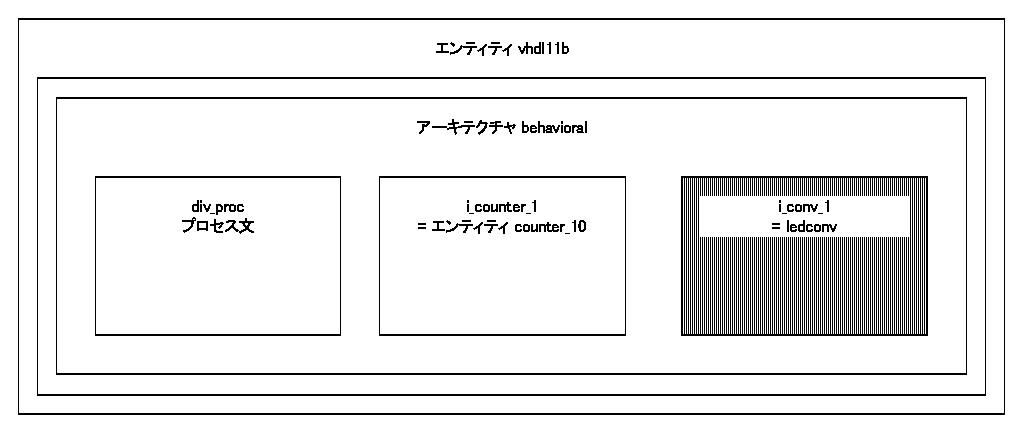
\includegraphics{figure27.eps}
\end{figure}

counter10 を呼び出しているときのキーワード ``i\_counter1'' や ledconv に対する ``i\_conv1'' がインスタンス名となります。固有のインスタンス名をつけることで、同じ回路ブロックを複数回呼び出すことができます。

ポートの接続はこのコードのように、左辺に呼び出される回路のポート名、=\textgreater{} をはさんで右辺に呼び出し側の port 名または signal 名を書き、カンマで区切ります。カンマは区切りなので最後の接続の後には書きません。


\section{5.14 状態遷移と、条件分岐 case ~ when ~}
\label{05_try:case-when}
例えばカップラーメンを食べようとした場合でも、(誰かが作ってくれる場合を除いて)手順があります。
\begin{enumerate}
\item {} 
カップラーメンの包装をといてふたを開けて小袋をとりだす。必要なものはここで入れる。

\item {} 
やかんに水を入れてコンロにかけて沸かす。

\item {} 
沸騰するのを待つ。

\item {} 
沸騰したら火を止めて、お湯をカップに注ぐ。

\item {} 
3分(または5分)待つ。

\item {} 
必要に応じて小袋の中身をカップに入れる。まぜる。

\item {} 
食べてよし。

\end{enumerate}

小袋が入ってなかったり電気ポットでお湯を沸かしたり、湯切りタイプだったりとバリエーションがありますが、オーソドックなものではこのように順番があり、例えば1、2は入れ替えたり並列に行ってもいいですが、基本的に手順通りに行います。

プログラミングもこういったところに似ていますが、このように手順通りに処理を行いたい場合、ソフトウェアと同様状態遷移の考え方を使います。

状態遷移は通常は図で状態間のつながりを描きながら設計をし、ソースコードには人間が考えながら書き込むしかありません(図を描くことでソースコードを出力してくれるツールもあります)。

ソースコード上で、各「状態」を数字で表しながらコーディングすることもできますが、各「状態」に名前をつけて管理しやすくすることができます。

( C 言語のenum と同じような働きです)

使い方はたとえば以下のようになります。

\begin{Verbatim}[commandchars=\\\{\}]
\PYG{k}{type} \PYG{n}{RAMEN} \PYG{k}{is} \PYG{p}{(}\PYG{n}{MAKE\PYGZus{}READY\PYGZus{}CUP}\PYG{p}{,} \PYG{n}{BOILWATER}\PYG{p}{,} \PYG{n}{POURWATER}\PYG{p}{,} \PYG{n}{WAIT\PYGZus{}MINUTES}\PYG{p}{,} \PYG{n}{READY\PYGZus{}TO\PYGZus{}EAT}\PYG{p}{)}\PYG{p}{;}
\PYG{k}{signal} \PYG{n}{ramen\PYGZus{}stat} \PYG{o}{:} \PYG{n}{RAMEN}\PYG{p}{;}
\PYG{k}{begin}
  \PYG{n}{ramen\PYGZus{}stat} \PYG{o}{\PYGZlt{}}\PYG{o}{=} \PYG{n}{MAKEREADY}\PYG{p}{;}
\end{Verbatim}

1行目では RAMEN という型を新しく定義しています。この型のとりうる値は''MAKE\_READY\_CUP''以降の5種類です。

2行目では、RAMEN の型の signal 、ramen\_stat を宣言します。

ramen\_stat には MAKE\_READY\_CUP など、定義した名前を代入したり、if 文で比較したりすることができます。ただし勝手に作った型ですので、そのままでは port から出力しても使えませんし、例えば LED の点灯パターンに対しては全く対応がとれないため使えません。あくまで内部で使うのが基本です。

このようにしなくても、自分でこれらの状態を管理すれば、たとえば integer の signal ででも管理できます。ただしわかりやすい名前をつけることで、ソースコードが理解しやすくなります。


\section{5.15 条件分岐 case ~ when ~}
\label{05_try:id23}
\begin{notice}{note}{注釈:}
case 文はprocess 文の中でのみ使用できます。

状態遷移専用ではありませんが、case 文はよく組み合わされて使われます。基本的な形は以下の通りです。
\end{notice}

\begin{Verbatim}[commandchars=\\\{\}]
case (CONDITION\PYGZus{}SIGNAL) is
  when (VALUE\PYGZus{}A) =\PYGZgt{} ~ EXPRESSION A ~
  when (VALUE\PYGZus{}B) =\PYGZgt{} ~ EXPRESSION B ~
  when others =\PYGZgt{} ~ EXPRESSION OTHER ~
end case;
\end{Verbatim}

ある一つの signal の値毎に処理を分岐させることができます。処理は、次の when まで何行でも書くことができます。


\subsection{5.15.1 演習}
\label{05_try:id24}
スイッチによって、特定のLED を点灯させる回路を作る。
* LED1 が点灯している場合、sw2 を操作することでLED1 が消灯し、LED2 が点灯する。
* LED2 が点灯している場合、sw1 を操作することで、LED2 が消灯し、LED1 が点灯する。sw2 を操作した場合は、LED2 が消灯し、LED3 が点灯する。
* LED3 が点灯している場合、sw1 を操作することで、LED3 が消灯し、LED2 が点灯する。

swfilter.vhd

\begin{Verbatim}[commandchars=\\\{\}]
\PYG{k}{library} \PYG{n+nn}{ieee} \PYG{p}{;}
\PYG{k}{use} \PYG{n+nn}{ieee.std\PYGZus{}logic\PYGZus{}1164.all}\PYG{p}{;}
\PYG{k}{use} \PYG{n+nn}{ieee.std\PYGZus{}logic\PYGZus{}arith.all}\PYG{p}{;}
\PYG{k}{use} \PYG{n+nn}{ieee.std\PYGZus{}logic\PYGZus{}unsigned.all}\PYG{p}{;}

\PYG{k}{entity} \PYG{n+nc}{swfilter} \PYG{k}{is}
  \PYG{k}{port} \PYG{p}{(}
    \PYG{n}{gclk0} \PYG{o}{:} \PYG{k}{in} \PYG{k+kt}{std\PYGZus{}logic}\PYG{p}{;}
    \PYG{n}{sw} \PYG{o}{:} \PYG{k}{in} \PYG{k+kt}{std\PYGZus{}logic}\PYG{p}{;}
    \PYG{n}{sw\PYGZus{}out} \PYG{o}{:} \PYG{k}{out} \PYG{k+kt}{std\PYGZus{}logic}
  \PYG{p}{)}\PYG{p}{;}
\PYG{k}{end} \PYG{n+nc}{swfilter}\PYG{p}{;}

\PYG{k}{architecture} \PYG{n+nc}{rtl} \PYG{k}{of} \PYG{n+nc}{swfilter} \PYG{k}{is}
  \PYG{k}{signal} \PYG{n}{c} \PYG{o}{:} \PYG{k+kt}{std\PYGZus{}logic\PYGZus{}vector} \PYG{p}{(}\PYG{l+m+mi}{14} \PYG{k}{downto} \PYG{l+m+mi}{0}\PYG{p}{)}\PYG{p}{;}
  \PYG{k}{signal} \PYG{n}{r} \PYG{o}{:} \PYG{k+kt}{std\PYGZus{}logic}\PYG{p}{;}
  \PYG{k}{signal} \PYG{n}{d1} \PYG{o}{:} \PYG{k+kt}{std\PYGZus{}logic}\PYG{p}{;}
  \PYG{k}{signal} \PYG{n}{d2} \PYG{o}{:} \PYG{k+kt}{std\PYGZus{}logic}\PYG{p}{;}
  \PYG{k}{signal} \PYG{n}{s} \PYG{o}{:} \PYG{k+kt}{std\PYGZus{}logic}\PYG{p}{;}
\PYG{k}{begin}
  \PYG{n}{sum\PYGZus{}proc} \PYG{o}{:} \PYG{k}{process} \PYG{p}{(}\PYG{n}{gclk0}\PYG{p}{)}
  \PYG{k}{begin}
    \PYG{k}{if} \PYG{p}{(}\PYG{n}{gclk0}\PYG{n+na}{\PYGZsq{}event} \PYG{k}{and} \PYG{n}{gclk0} \PYG{o}{=} \PYG{l+s+sc}{\PYGZsq{}1\PYGZsq{}}\PYG{p}{)} \PYG{k}{then}
      \PYG{k}{if} \PYG{p}{(}\PYG{n}{sw} \PYG{o}{=} \PYG{l+s+sc}{\PYGZsq{}0\PYGZsq{}}\PYG{p}{)} \PYG{k}{then}
        \PYG{n}{c} \PYG{o}{\PYGZlt{}}\PYG{o}{=} \PYG{l+s}{\PYGZdq{}000000000000000\PYGZdq{}}\PYG{p}{;}
      \PYG{k}{elsif} \PYG{p}{(}\PYG{p}{(}\PYG{n}{c} \PYG{o}{/}\PYG{o}{=} \PYG{l+s}{\PYGZdq{}111111111111111\PYGZdq{}}\PYG{p}{)} \PYG{k}{and} \PYG{p}{(}\PYG{n}{sw} \PYG{o}{=} \PYG{l+s+sc}{\PYGZsq{}1\PYGZsq{}}\PYG{p}{)}\PYG{p}{)} \PYG{k}{then}
        \PYG{n}{c} \PYG{o}{\PYGZlt{}}\PYG{o}{=} \PYG{n}{c} \PYG{o}{+} \PYG{l+m+mi}{1}\PYG{p}{;}
      \PYG{k}{end} \PYG{k}{if}\PYG{p}{;}

      \PYG{k}{if} \PYG{p}{(}\PYG{n}{c} \PYG{o}{=} \PYG{l+s}{\PYGZdq{}111111111111111\PYGZdq{}}\PYG{p}{)} \PYG{k}{then}
        \PYG{n}{r} \PYG{o}{\PYGZlt{}}\PYG{o}{=} \PYG{l+s+sc}{\PYGZsq{}1\PYGZsq{}}\PYG{p}{;}
      \PYG{k}{else}
        \PYG{n}{r} \PYG{o}{\PYGZlt{}}\PYG{o}{=} \PYG{l+s+sc}{\PYGZsq{}0\PYGZsq{}}\PYG{p}{;}
      \PYG{k}{end} \PYG{k}{if}\PYG{p}{;}
    \PYG{k}{end} \PYG{k}{if}\PYG{p}{;}
  \PYG{k}{end} \PYG{k}{process}\PYG{p}{;}

  \PYG{n}{diff\PYGZus{}proc} \PYG{o}{:} \PYG{k}{process} \PYG{p}{(}\PYG{n}{gclk0}\PYG{p}{)}
  \PYG{k}{begin}
    \PYG{k}{if} \PYG{p}{(}\PYG{n}{gclk0}\PYG{n+na}{\PYGZsq{}event} \PYG{k}{and} \PYG{n}{gclk0} \PYG{o}{=} \PYG{l+s+sc}{\PYGZsq{}1\PYGZsq{}}\PYG{p}{)} \PYG{k}{then}
      \PYG{n}{d1} \PYG{o}{\PYGZlt{}}\PYG{o}{=} \PYG{n}{r}\PYG{p}{;}
      \PYG{n}{d2} \PYG{o}{\PYGZlt{}}\PYG{o}{=} \PYG{n}{d1}\PYG{p}{;}
      \PYG{n}{s} \PYG{o}{\PYGZlt{}}\PYG{o}{=} \PYG{n}{d1} \PYG{k}{and} \PYG{p}{(}\PYG{k}{not} \PYG{n}{d2}\PYG{p}{)}\PYG{p}{;}
    \PYG{k}{end} \PYG{k}{if}\PYG{p}{;}
  \PYG{k}{end} \PYG{k}{process}\PYG{p}{;}

  \PYG{n}{sw} \PYG{k}{out} \PYG{o}{\PYGZlt{}}\PYG{o}{=} \PYG{n}{s}\PYG{p}{;}
\PYG{k}{end} \PYG{n+nc}{rtl}\PYG{p}{;}
\end{Verbatim}

プロジェクト名 vhdl12

vhdl12.vhd

\begin{Verbatim}[commandchars=\\\{\}]
\PYG{k}{library} \PYG{n+nn}{ieee}\PYG{p}{;}
\PYG{k}{use} \PYG{n+nn}{ieee.std\PYGZus{}logic\PYGZus{}1164.all}\PYG{p}{;}
\PYG{k}{use} \PYG{n+nn}{ieee.std\PYGZus{}logic\PYGZus{}arith.all}\PYG{p}{;}
\PYG{k}{use} \PYG{n+nn}{ieee.std\PYGZus{}logic\PYGZus{}unsigned.all}\PYG{p}{;}

\PYG{k}{entity} \PYG{n+nc}{vhdl12} \PYG{k}{is}
  \PYG{k}{port} \PYG{p}{(}
    \PYG{n}{gclk0} \PYG{o}{:} \PYG{k}{in} \PYG{k+kt}{std\PYGZus{}logic}\PYG{p}{;}
    \PYG{n}{sw1} \PYG{o}{:} \PYG{k}{in} \PYG{k+kt}{std\PYGZus{}logic}\PYG{p}{;}
    \PYG{n}{sw2} \PYG{o}{:} \PYG{k}{in} \PYG{k+kt}{std\PYGZus{}logic}\PYG{p}{;}
    \PYG{n}{led1} \PYG{o}{:} \PYG{k}{out} \PYG{k+kt}{std\PYGZus{}logic}\PYG{p}{;}
    \PYG{n}{led2} \PYG{o}{:} \PYG{k}{out} \PYG{k+kt}{std\PYGZus{}logic}\PYG{p}{;}
    \PYG{n}{led3} \PYG{o}{:} \PYG{k}{out} \PYG{k+kt}{std\PYGZus{}logic}
  \PYG{p}{)}\PYG{p}{;}
\PYG{k}{end} \PYG{n+nc}{vhdl12}\PYG{p}{;}

\PYG{k}{architecture} \PYG{n+nc}{rtl} \PYG{k}{of} \PYG{n+nc}{vhdl12} \PYG{k}{is}
  \PYG{k}{component} \PYG{n+nc}{swfilter}
    \PYG{k}{port} \PYG{p}{(}
      \PYG{n}{gclk0} \PYG{o}{:} \PYG{k}{in} \PYG{k+kt}{std\PYGZus{}logic}\PYG{p}{;}
      \PYG{n}{sw} \PYG{o}{:} \PYG{k}{in} \PYG{k+kt}{std\PYGZus{}logic}\PYG{p}{;}
      \PYG{n}{sw\PYGZus{}out} \PYG{o}{:} \PYG{k}{out} \PYG{k+kt}{std\PYGZus{}logic}
    \PYG{p}{)}\PYG{p}{;}
  \PYG{k}{end} \PYG{k}{component}\PYG{p}{;}

  \PYG{k}{signal} \PYG{n}{sw1d} \PYG{o}{:} \PYG{k+kt}{std\PYGZus{}logic}\PYG{p}{;}
  \PYG{k}{signal} \PYG{n}{sw2d} \PYG{o}{:} \PYG{k+kt}{std\PYGZus{}logic}\PYG{p}{;}

  \PYG{k}{type} \PYG{n}{LED\PYGZus{}STAT} \PYG{k}{is} \PYG{p}{(}\PYG{n}{P} \PYG{n}{LED1}\PYG{p}{,} \PYG{n}{P} \PYG{n}{LED2}\PYG{p}{,} \PYG{n}{P} \PYG{n}{LED3}\PYG{p}{)}\PYG{p}{;}
  \PYG{k}{signal} \PYG{n}{lstat} \PYG{o}{:} \PYG{n}{LED\PYGZus{}STAT}\PYG{p}{;}

  \PYG{k}{signal} \PYG{n}{led} \PYG{o}{:} \PYG{k+kt}{std\PYGZus{}logic\PYGZus{}vector} \PYG{p}{(}\PYG{l+m+mi}{3} \PYG{k}{downto} \PYG{l+m+mi}{1}\PYG{p}{)}\PYG{p}{;}
\PYG{k}{begin}
  \PYG{n}{sw1\PYGZus{}filter} \PYG{o}{:} \PYG{n}{swfilter}
    \PYG{k}{port} \PYG{k}{map} \PYG{p}{(}
      \PYG{n}{gclk0} \PYG{o}{=}\PYG{o}{\PYGZgt{}} \PYG{n}{gclk0}\PYG{p}{,}
      \PYG{n}{sw} \PYG{o}{=}\PYG{o}{\PYGZgt{}} \PYG{n}{sw1}\PYG{p}{,}
      \PYG{n}{sw\PYGZus{}out} \PYG{o}{=}\PYG{o}{\PYGZgt{}} \PYG{n}{sw1d}
    \PYG{p}{)}\PYG{p}{;}

  \PYG{n}{sw2\PYGZus{}filter} \PYG{o}{:} \PYG{n}{swfilter}
    \PYG{k}{port} \PYG{k}{map} \PYG{p}{(}
      \PYG{n}{gclk0} \PYG{o}{=}\PYG{o}{\PYGZgt{}} \PYG{n}{gclk0}\PYG{p}{,}
      \PYG{n}{sw} \PYG{o}{=}\PYG{o}{\PYGZgt{}} \PYG{n}{sw2}\PYG{p}{,}
      \PYG{n}{sw\PYGZus{}out} \PYG{o}{=}\PYG{o}{\PYGZgt{}} \PYG{n}{sw2d}
    \PYG{p}{)}\PYG{p}{;}

  \PYG{n}{stat\PYGZus{}proc} \PYG{o}{:} \PYG{k}{process} \PYG{p}{(}\PYG{n}{gclk0}\PYG{p}{)}
  \PYG{k}{begin}
    \PYG{k}{if} \PYG{p}{(}\PYG{n}{gclk0}\PYG{n+na}{\PYGZsq{}event} \PYG{k}{and} \PYG{n}{gclk0} \PYG{o}{=} \PYG{l+s+sc}{\PYGZsq{}1\PYGZsq{}}\PYG{p}{)} \PYG{k}{then}
      \PYG{k}{case} \PYG{n}{lstat} \PYG{k}{is}
        \PYG{k}{when} \PYG{n}{P} \PYG{n}{LED1} \PYG{o}{=}\PYG{o}{\PYGZgt{}}
          \PYG{k}{if} \PYG{p}{(}\PYG{n}{sw2d} \PYG{o}{=} \PYG{l+s+sc}{\PYGZsq{}1\PYGZsq{}}\PYG{p}{)} \PYG{k}{then}
            \PYG{n}{lstat} \PYG{o}{\PYGZlt{}}\PYG{o}{=} \PYG{n}{P} \PYG{n}{LED2}\PYG{p}{;}
          \PYG{k}{end} \PYG{k}{if}\PYG{p}{;}
          \PYG{n}{led} \PYG{o}{\PYGZlt{}}\PYG{o}{=} \PYG{l+s}{\PYGZdq{}001\PYGZdq{}}\PYG{p}{;}

        \PYG{k}{when} \PYG{n}{P} \PYG{n}{LED2} \PYG{o}{=}\PYG{o}{\PYGZgt{}}
          \PYG{k}{if} \PYG{p}{(}\PYG{n}{sw1d} \PYG{o}{=} \PYG{l+s+sc}{\PYGZsq{}1\PYGZsq{}}\PYG{p}{)} \PYG{k}{then}
            \PYG{n}{lstat} \PYG{o}{\PYGZlt{}}\PYG{o}{=} \PYG{n}{P} \PYG{n}{LED1}\PYG{p}{;}
          \PYG{k}{elsif} \PYG{p}{(}\PYG{n}{sw2d} \PYG{o}{=} \PYG{l+s+sc}{\PYGZsq{}1\PYGZsq{}}\PYG{p}{)} \PYG{k}{then}
            \PYG{n}{lstat} \PYG{o}{\PYGZlt{}}\PYG{o}{=} \PYG{n}{P} \PYG{n}{LED3}\PYG{p}{;}
          \PYG{k}{end} \PYG{k}{if}\PYG{p}{;}
          \PYG{n}{led} \PYG{o}{\PYGZlt{}}\PYG{o}{=} \PYG{l+s}{\PYGZdq{}010\PYGZdq{}}\PYG{p}{;}

        \PYG{k}{when} \PYG{n}{P} \PYG{n}{LED3} \PYG{o}{=}\PYG{o}{\PYGZgt{}}
          \PYG{k}{if} \PYG{p}{(}\PYG{n}{sw1d} \PYG{o}{=} \PYG{l+s+sc}{\PYGZsq{}1\PYGZsq{}}\PYG{p}{)} \PYG{k}{then}
            \PYG{n}{lstat} \PYG{o}{\PYGZlt{}}\PYG{o}{=} \PYG{n}{P} \PYG{n}{LED2}\PYG{p}{;}
          \PYG{k}{end} \PYG{k}{if}\PYG{p}{;}
          \PYG{n}{led} \PYG{o}{\PYGZlt{}}\PYG{o}{=} \PYG{l+s}{\PYGZdq{}100\PYGZdq{}}\PYG{p}{;}

        \PYG{k}{when} \PYG{k}{others} \PYG{o}{=}\PYG{o}{\PYGZgt{}}
          \PYG{n}{lstat} \PYG{o}{\PYGZlt{}}\PYG{o}{=} \PYG{n}{P} \PYG{n}{LED1}\PYG{p}{;}
          \PYG{n}{led} \PYG{o}{\PYGZlt{}}\PYG{o}{=} \PYG{l+s}{\PYGZdq{}111\PYGZdq{}}\PYG{p}{;}
      \PYG{k}{end} \PYG{k}{case}\PYG{p}{;}
    \PYG{k}{end} \PYG{k}{if}\PYG{p}{;}
  \PYG{k}{end} \PYG{k}{process}\PYG{p}{;}

  \PYG{n}{led1} \PYG{o}{\PYGZlt{}}\PYG{o}{=} \PYG{k}{not} \PYG{n}{led} \PYG{p}{(}\PYG{l+m+mi}{1}\PYG{p}{)}\PYG{p}{;}
  \PYG{n}{led2} \PYG{o}{\PYGZlt{}}\PYG{o}{=} \PYG{k}{not} \PYG{n}{led} \PYG{p}{(}\PYG{l+m+mi}{2}\PYG{p}{)}\PYG{p}{;}
  \PYG{n}{led3} \PYG{o}{\PYGZlt{}}\PYG{o}{=} \PYG{k}{not} \PYG{n}{led} \PYG{p}{(}\PYG{l+m+mi}{3}\PYG{p}{)}\PYG{p}{;}
\PYG{k}{end} \PYG{n+nc}{rtl}\PYG{p}{;}
\end{Verbatim}

case 文とは関係ありませんが、sw lter はsw にスイッチからの信号を接続し、sw outにチャタリング除去後の信号を出力する回路ブロックです。


\section{5.16 ストップウォッチ}
\label{05_try:id25}
1/100 秒単位のストップウォッチを実装する。

表示は4桁の7セグLED で行い、10進数のカウントで、99.99 秒までカウントできること。


\subsection{5.16.1 課題:最小限の構成}
\label{05_try:id26}
ラップ・スプリット機能の無いストップウォッチを実装する。

操作は2つのスイッチで行う。

スタート・ストップ押す毎にカウント動作とストップを切り替える。

カウント動作中に押してストップした後、再度押した場合、続きからカウント動作を行う。

リセット押すとカウントしていた値をクリアする。

カウント動作中に押した場合の動作は定義しない(どのように動作してもよい)。

99.99 秒の次のカウントは未定義(どのように動作してもよい)。


\subsubsection{5.16.1.1 ヒント}
\label{05_try:id27}
vhdl11b の10進カウンタcounter10 、7 セグLED への変換を行う ledconv 、vhdl12のチャタリング除去回路 swfilter が応用できる。

今カウント中なのか止まっているのか、判定する signal を作って制御する。


\subsection{5.16.2 課題:応用}
\label{05_try:id28}
ラップ、またはスプリット、または両方の機能のついたストップウォッチを実装する。

操作は2つのスイッチで行う。

スタート・ストップ押す毎にカウント動作とストップを切り替える。

カウント動作中に押してストップした後、再度押した場合、続きからカウント動作を行う。

ラップ/スプリット・リセット押したときの動作状況に合わせて、このスイッチの動作も変化する。

カウントがストップしている時に押すとリセット動作として、カウントしていた値をクリアする。

カウント動作中に押すとスプリット動作として、表示している値を止める。カウント動作は継続する。

スプリット状態で再度押した場合、カウントしている値の表示を再開する。

カウント動作中にスイッチを押して表示を止め、ストップボタンでカウントを停止しても表示は維持する。

その状態でこのスイッチを押すと、カウントがストップした値を表示する。

この状態でもう一度このスイッチを押すと、カウントはクリアする(リセット)その前にスタートのスイッチを押すと、その値からカウントを再開する。

ラップの場合、ボタンを押すと表示している値をとめ、カウントは0から再開する。

ラップ機能、スプリット機能を両方実装する場合は、スイッチの一つをモードの切り替えに割り振る。

99.99 秒の次のカウントは00.00 秒とする。


\subsubsection{5.16.2.1 ヒント}
\label{05_try:id29}
現在どの状況にいるのかを保持するシグナルか状態遷移を応用する。


\subsection{5.16.3 その他課題}
\label{05_try:id30}
タイマーを作成する。

表示は、上位2桁が「分」、下位2桁が「秒」とする。

第一段階は、決められた時間(たとえば3分など)のカウントダウンを行う。0までカウントダウンが完了したらそこで停止する。

リセットするとカウントする時間をリロードする。

第二段階は、カウントする時間を2つから選べるようにする(たとえば3分と5分)。

最後は、任意の時間を設定できるようにする。


\chapter{第6章 付録}
\label{06_appendix:id1}\label{06_appendix::doc}

\section{6.1 参考情報}
\label{06_appendix:id2}
VHDL Language Reference Manual 言語の規格

\href{http://ieeexplore.ieee.org/xpl/freeabs}{http://ieeexplore.ieee.org/xpl/freeabs} all.jsp?reload=true\&arnumber=4772740

VHDL によるハードウェア設計入門

CQ 出版/ 長谷川裕恭著

HDL サンプル記述集

CQ 出版

トランジスタ技術SPECIAL No. 79 初歩のHDL 設計学習帳

CQ 出版

トランジスタ技術SPECIAL for フレッシャーズNo. 105 ロジック回路設計はじめの一歩

CQ 出版

例題で学ぶ論理回路設計

森北出版/ 富川武彦著

ディジタルコンピューティングシステム

昭晃堂/ 亀山充隆著


\chapter{Indices and tables}
\label{index:indices-and-tables}\begin{itemize}
\item {} 
\DUspan{xref,std,std-ref}{genindex}

\item {} 
\DUspan{xref,std,std-ref}{modindex}

\item {} 
\DUspan{xref,std,std-ref}{search}

\end{itemize}



\renewcommand{\indexname}{索引}
\printindex
\end{document}
